\documentclass[openany,oneside,12pt,a4paper]{UoP_template}
%\documentclass[oneside,a4paper,12pt]{../Common/Thesis_UoP}
%\usepackage[square, numbers, comma, sort&compress]{natbib} % option clash with many
\usepackage{etex} % has to be just after the documentclass, so first here
\usepackage[export]{adjustbox}
\usepackage{algorithm}
\usepackage{algorithmic}
%\usepackage{algcompatible}
\usepackage{amssymb}
\usepackage{amsmath}
\usepackage[toc,page,titletoc]{appendix}
\usepackage{booktabs}
\usepackage{calc}
\usepackage[font=small,skip=0pt]{caption}
\usepackage{float}
\usepackage{csvsimple}
\usepackage{dirtree}
\usepackage{enumitem}
%\usepackage{epigraph} % TuDelf redefine error
\usepackage{epstopdf}
%\usepackage[paperwidth=21cm, paperheight=29.7cm,top=15mm, bottom=22mm, left=50mm, right=10mm]{geometry} %dont use, overrides many options
\usepackage{graphicx}
\usepackage{indentfirst}
\usepackage{listings}
\usepackage{longtable}
%\usepackage[square, numbers, comma, sort&compress]{natbib} % option clash with many
\usepackage{rotating}
\usepackage{subfig} %BAD LIST OF FIGURES, BUT NEEDED FOR SUBFLOAT
%\usepackage{subfigure} % deprecated, don't use
\usepackage{textcomp}
%\usepackage{tocloft}
\usepackage{tikz-qtree} 
%%%\usepackage{titlesec} % for subsubsubsection May 2016, updated caused MISSING COUNT ERROR
%\usepackage{todonotes}
\usepackage{url}
\usepackage{vector}
\usepackage{verbatim}
\usepackage{xcolor}

\setlength{\abovecaptionskip}{4pt} % Chosen fairly arbitrarily
%\setlength{\belowcaptionskip}{4pt} % Chosen fairly arbitrarily
\setlength{\textfloatsep}{1.5pt plus 1.0pt minus 2.0pt}
\setlength{\floatsep}{1.5pt plus 1.0pt minus 2.0pt}
\setlength{\intextsep }{1.5pt plus 1.0pt minus 2.0pt}
\newtheorem{mydef}{Definition}
\newtheorem{mylem}{Remark}
\newtheorem{myhyp}{Hypothesis}


\pdfminorversion=5
\pdfobjcompresslevel=3 
\pdfcompresslevel=9

% NO LINK COLORS
\hypersetup{
    colorlinks,
    citecolor=black,
    filecolor=black,
    linkcolor=black,
    urlcolor=black
}

\title{DEVELOPMENT OF ALGORITHMS FOR GENERATING CONNECTED MIDSURFACES USING FEATURE INFORMATION IN THIN-WALLED PARTS} % HAS TO BE IN CAPITAL LETTERS
\degree{DOCTOR OF PHILOSOPHY (PH.D)}
\degreedate{\today}
\author{YOGESH H. KULKARNI}
\collegeordept{Department of Mechanical Engineering}
\university{SAVITRIBAI PHULE PUNE UNIVERSITY}
\subject{MECHANICAL ENGINEERING}
\guide{DR. ANIL SAHASRABUDHE AND DR. MUKUND KALE}
\guideinstitute{COLLEGE OF ENGINEERING , PUNE}

% turn of those nasty overfull and underfull hboxes
\hbadness=10000
\hfuzz=50pt

\newcommand{\myquote}[2]{
\hfill \begin{minipage}[r]{0.4\linewidth}
%\raggedright{\em ``#1''} \\
%\raggedright{- #2}\\
\begin{flushright}
{\em ``#1''} \\  {- #2} \\
\end{flushright}

\textcolor{gray}{\rule{\linewidth}{0.8mm}}
\end{minipage}
}

\newcommand{\loft}[5]{\ensuremath{\textcolor{black}{\Omega{\bf \mathcal{L}}_{#1}^{#2,#3}}[\textcolor{black}{\{#4\}}\textcolor{black}{(#5)}]}}

\newcommand{\affine}[5]{\ensuremath{\textcolor{black}{\Delta{\bf \mathcal{A}}_{#1}^{#2,#3}} [\textcolor{black}{\{#4\}} \textcolor{black}{(#5)}]}}

\newcommand{\boolop}[5]{\ensuremath{\textcolor{black}{\Omega{\bf \mathcal{B}}_{#1}^{#2,#3}}[\textcolor{black}{\{#4\}} \textcolor{black}{(#5)}]}}

\newcommand{\generic}[7]{\ensuremath{\textcolor{black}{#1{\bf \mathcal{#2}}_{#3}^{#4,#5}}[\textcolor{black}{\{#6\}} \textcolor{black}{(#7)}]}}


%\newcommand{\loft}[5]{\ensuremath{\textcolor{magenta}{\Omega{\bf \mathcal{L}}_{#1}^{#2,#3}}[\textcolor{blue}{\{#4\}}\textcolor{red}{(#5)}]}}
%
%\newcommand{\affine}[5]{\ensuremath{\textcolor{magenta}{\Delta{\bf \mathcal{A}}_{#1}^{#2,#3}} [\textcolor{blue}{\{#4\}} \textcolor{red}{(#5)}]}}
%
%\newcommand{\boolop}[5]{\ensuremath{\textcolor{magenta}{\Omega{\bf \mathcal{B}}_{#1}^{#2,#3}}[\textcolor{blue}{\{#4\}} \textcolor{red}{(#5)}]}}
%
%\newcommand{\generic}[7]{\ensuremath{\textcolor{magenta}{#1{\bf \mathcal{#2}}_{#3}^{#4,#5}}[\textcolor{blue}{\{#6\}} \textcolor{red}{(#7)}]}}

%\newcommand{\loft}[5]{\ensuremath{\Omega{\bf \mathcal{L}}_{#1}^{#2,#3}}[\{#4\} (#5)]}
%
%\newcommand{\affine}[5]{\ensuremath{\Delta{\bf \mathcal{A}}_{#1}^{#2,#3} [\{#4\} (#5)]}}
%
%\newcommand{\boolop}[5]{\ensuremath{\Omega{\bf \mathcal{B}}_{#1}^{#2,#3}[\{#4\} (#5)]}}
%
%\newcommand{\generic}[7]{\ensuremath{#1 {\bf \mathcal{#2}}_{#3}^{#4,#5}[\{#6\} (#7)]}}

%\makeatletter
%\renewcommand{\l@figure}{\@dottedtocline{1}{1.5em}{4em}}
%\makeatother

\newcommand{\mysystemname}{$\mathbf{MidAS}$}
\onehalfspacing

\usepackage[explicit]{titlesec}
\titleformat{\chapter}[display]{\bfseries \centering}{\huge Chapter \thechapter}{1em}{\Huge #1}

\setcounter{secnumdepth}{3}
\setcounter{tocdepth}{3}


\begin{document}

%\clearpage
%\thispagestyle{empty}
%\pagenumbering{gobble}% Remove page numbers (and reset to 1)
%\pagenumbering{roman}
%
%\clearpage
%\thispagestyle{empty}
%
\frontmatter % book mode only: turns off chapter numbering and uses roman numerals for page numbers;

\maketitle

\pagebreak  \thispagestyle{empty}
\topskip0pt
\vspace*{0.25\textheight}
\begin{center}
To my parents...
\end{center}
\vspace*{\fill}

  
\addcontentsline{toc}{chapter}{Dedication}

%\pagebreak \thispagestyle{empty}
%\begin{figure} [!h]
	\centering
	\includegraphics[width=\linewidth]{..//Common/images/coep_header.png}
\end{figure}

\vspace*{50pt}

\begin{center}{\Huge \textbf{Certificate of the Guide}}\end{center}

\vspace*{20pt}

\begin{flushleft}
CERTIFIED that the work incorporated in the thesis entitled  \textcolor{blue}{\textbf{``Development of Algorithms for Generating Connected Midsurfaces Using Feature Information in Thin-walled Parts''}}, submitted by \textcolor{red}{\textbf{Mr. Yogesh H. Kulkarni}} was carried out by the candidate under my supervision/guidance. Such material as has been obtained from other sources has been duly acknowledged in the thesis. 
\end{flushleft}

\vspace*{120pt}


\begin{minipage}[t]{0.5\textwidth}%
\begin{flushleft}
 Dr. Mukund Kale\\
\emph{Co-Guide}\\
Siemens PLM India, Pune.
\end{flushleft}
\end{minipage}\hspace{0.5cm}
\begin{minipage}[t]{0.4\textwidth}%
\begin{flushleft}
 {
Dr. Anil Sahasrabudhe \\
\emph{Guide}}\\
College of Engineering, Pune.
\end{flushleft}
\end{minipage}
%
%
%\begin{minipage}[t]{0.5\textwidth}%
%\begin{tabular}{lcl}
%Date & : & \today \tabularnewline
%Place &: &  \tabularnewline
%\end{tabular}%
%\end{minipage}
%
%\begin{minipage}[t]{0.5\textwidth}%
%\begin{tabular}{lcl}
%Date & : &  \tabularnewline
%Place &: &  \tabularnewline
%\end{tabular}%
%\end{minipage}



%\addcontentsline{toc}{chapter}{Certificate of the Guide}
%
%\pagebreak \thispagestyle{empty}
%\begin{figure} [!h]
	\centering
	\includegraphics[width=\textwidth]{..//Common/images/coep_header.png}
\end{figure}

\vspace*{50pt}

\begin{center}{\Huge \textbf{Certificate}}\end{center}

\vspace*{20pt}

\begin{flushleft}
This is to certify that the thesis, entitled \textcolor{blue}{\textbf{``Development of Algorithms for Generating Connected Midsurfaces Using Feature Information in Thin-walled Parts''}}, submitted by \textcolor{red}{\textbf{Yogesh H. Kulkarni}} in partial fulfillment of requirement for the award of the degree of Doctor of Philosophy in Mechanical Engineering at College of Engineering, Pune, during the session 2016-17, is a bonafide record of the work carried out by him. He has worked under my supervision and guidance and has fulfilled the requirement of submission of the thesis. The matter embodied in this thesis has not been submitted elsewhere in part or full for the award of any Degree or Diploma.
\end{flushleft}

\vspace*{120pt}

\begin{minipage}[t]{0.5\textwidth}%
\begin{flushleft}
 \textcolor{blue}{\textbf{Dr. Mukund Kale}}\\
\emph{Co-Guide}\\
Siemens PLM India, Pune.
\end{flushleft}
\end{minipage}\hspace{0.5cm}
\begin{minipage}[t]{0.4\textwidth}%
\begin{flushleft}
 {
\textcolor{blue}{\textbf{Dr. Anil Sahasrabudhe}}\\
\emph{Research Guide}}\\
College of Engineering, Pune.
\end{flushleft}

\end{minipage}

\vfill
\begin{minipage}[t]{0.5\textwidth}%
\begin{flushleft}
\textcolor{blue}{\textbf{Dr. S. N. Sapali}}\\
\emph{Head of Mechanical Engineering}\\
College of Engineering, Pune.
\end{flushleft}
\end{minipage}\hspace{0.5cm}
\begin{minipage}[t]{0.4\textwidth}%
\begin{flushleft}
\textcolor{blue}{\textbf{Dr. B. B. Ahuja}}\\
\emph{Director}\\
College of Engineering, Pune.
\end{flushleft}

\end{minipage}
%\addcontentsline{toc}{chapter}{Certificate}
%
%\pagebreak \thispagestyle{empty}
%\begin{figure} [!h]
	\centering
	\includegraphics[width=\linewidth]{images/coep_header.png}
\end{figure}

\vspace*{50pt}

\begin{center}{\Huge \textbf{Declaration by the Candidate}}\end{center}

\vspace*{20pt}

\begin{flushleft}
I declare that the thesis entitled \textcolor{blue}{\textbf{``Development of Algorithms for Generating Connected Midsurfaces Using Feature Information in Thin-walled Parts''}}, submitted by me for the degree of Doctor of Philosophy is the record of work carried out by me during the period from 13th August 2012 to till date of preparation of this thesis under the guidance of \textcolor{blue}{\textbf{Dr. Anil Sahasrabudhe}} and \textcolor{blue}{\textbf{Dr. Mukund Kale}} and has not formed the basis for the award of any degree, diploma, associateship, fellowship, titles in this or any other University or other institution of Higher learning.
I further declare that the material obtained from other sources has been duly acknowledged in the thesis.

\end{flushleft}

\vspace*{120pt}

\begin{minipage}[t]{0.5\textwidth}%
\begin{tabular}{lcl}
Date & : &  \tabularnewline
Place &: &  \tabularnewline
\end{tabular}%
\end{minipage}\hspace{0.5cm}
\begin{minipage}[t]{0.4\textwidth}%
\begin{flushleft}
 {
\textcolor{blue}{\textbf{Yogesh H. Kulkarni}}\\
\emph{Ph.D. Candidate}}\\
College of Engineering, Pune.
\end{flushleft}

\end{minipage}
 
%\addcontentsline{toc}{chapter}{Declaration of the Candidate}

\pagebreak %\newpage %\thispagestyle{empty}
\addcontentsline{toc}{chapter}{Abstract}
\chapter*{Abstract}
%Paragraph 1: What is the problem? Not more than 3-4 sentences telling the reader what the problem is, in as simple English as possible
%Paragraph 2: Why is the problem hard? What has eluded us in solving it? What does the literature say about this problem?  What are the obstacles/challenges? Why is it non-trivial? 
%Paragraph 3: What is your approach/result to solving this problem?   How come you solved it? Think of this as your “startling” or “sit up and take notice” claims that your thesis will plan to prove/demonstrate 
%Paragraph 4: What is the consequence of your approach? So, now that you’ve made me sit up and take notice, what is the impact? What does your approach/result enable?  


Computer-aided Design (CAD) models of thin-walled solids such as sheet metal or plastic parts are often reduced dimensionally to their corresponding midsurfaces for quicker and fairly accurate results of Computer-aided Engineering (CAE) analysis.  A midsurface is a surface lying midway of (and representing) the input shape.  Computation of the midsurface is still a time-consuming and mostly, a manual task due to lack of robust-automated approaches. Many of the existing automatic midsurface generation approaches result in some kind of failures such as gaps, missing patches, overlapping surfaces, etc. It takes hours or even days to correct such errors with manual intervention. The widely used Boundary Representation (Brep) based approaches are computationally intensive, yet cannot guarantee flawless midsurface and are mostly developed for a limited variety of geometric and topological configurations.  In these approaches no feature information is efficiently leveraged. Thus, there exists a need to take a holistic look at the CAD model with its feature information and devise a set of efficient algorithms to generate flawless, well-connected midsurfaces capable of handling wide variety of geometric and topological configurations and are also computationally inexpensive. %Thus, an automatic, generalized and deterministic algorithm for computation of a well-connected midsurface is the need of the hour.
%Most of the existing approaches work on the final shape (typically in the form of Boundary representation, B-rep). Complex B-reps make it hard to detect sub-shapes for which the midsurface patches are computed and joined, forcing the usage of hard-coded geometric/heuristic rules, developed on a case-to-case basis. The research presented here proposes to address these problems by leveraging feature-information made available from the modern CAD applications. 

This thesis is primarily aimed at addressing this need. It provides an integrated approach to address the critical aspects of generation of midsurface for feature based sheet metal CAD model through design and implementation of an intelligent system, called \mysystemname~({\bf Mid}surface {\bf A}lgorithms for {\bf S}heet-metal-parts). It uses CAD models built using Autodesk Inventor and its Application Programming Interfaces (APIs) are used to interact with the model. The algorithms for various modules are implemented in VB and C\# .Net programming languages.
%
%Features carry a higher level information (such as designer's intent, dependencies, parameters, etc.) than what's available in the solid (Brep). In the past, they were hidden due to proprietary reasons, but now have started becoming available through Application Programming Interfaces (APIs). Feature information can be leveraged effectively in the existing CAD algorithms, where some sort of feature recognition used to happen before proceeding with the core algorithm. In this work, algorithms for model-simplification, decomposition and midsurface generation, use feature information advantageously. 

The thesis begins by providing an overview of CAD-CAE process, relevance of midsurface in case of CAE analysis of thin-walled parts and describing motivation of choosing the topic of midsurface computation for research. It reviews traditional approaches for generating midsurfaces, comments on their advantages and limitations and brings out the critical gaps. Research objectives are laid down based on the literature review and gap analysis. Then the overview of proposed \mysystemname~is presented. 

It begins with defeaturing of the input CAD model. Irrelevant features are removed based on criteria such as sheet metal feature type, size of remnant feature portions. Apart from this, bulk negative features, called ``dormant'' features, are removed temporarily so as to simplify the CAD model without compromising on the gross shape. These dormant features are later reapplied on the generated midsurface. 

The defeatured model is further simplified by transforming the remaining sheet metal features into generalized features, representing variations of Loft feature. This generalized representation, called ``$\mathcal{ABLE}$ ({\bf A}ffine transformation, {\bf B}ooleans,  {\bf L}ofts and {\bf E}ntities)'' helps simplify the model further so that generic algorithms can be developed for generating midsurface. 

The $\mathcal{ABLE}$ model is simplified further by cellular decomposition. The cells are classified into solid and interface cells. They are delegated with the tasks of creating midsurface patches and joining them, respectively. Midsurface patches are created either by offsetting the profile face or by lofting midcurves of the profiles along the guide of the owner loft feature. Midcurve of the profile is computed by first, approximating it to polygon, then decomposing the polygon and finally, generating midcurves for each sub-polygons. Midsurface patches are joined in the interface cells by a generic logic to form a connected midsurface. The quality of output midsurface is assessed by a topological validation method which is proposed in this research. Towards the end, capabilities of \mysystemname~are demonstrated with real-life sheet metal part models. The thesis concludes by highlighting the major contributions and directions for the future work.

%In the proposed approach, first, the irrelevant features are identified and removed from the input model to compute its simplified gross shape. Remaining features, then undergo abstraction-transformation to become their corresponding generic Loft-based equivalents, each having a profile and a guide curve. The model is then decomposed into cell bodies and a graph is populated with each of the cell bodies of the nodes and fully-overlapping-surface-interfaces at the edges. The nodes are classified into midsurface-patch generating nodes (called `solid cells' or $sCell$s) and interaction-resolving nodes (interface cells' or $iCell$s). In $sCell$, a midsurface patch is generated by sweeping the midcurve of the owner-Loft-feature's profile along with its guide curve. Midsurface patches are then connected in the $iCell$s in a generic manner, thus resulting in a well-connected midsurface with minimum failures. Output midsurface is then validated topologically for correctness. At the end, practical, real-life case-studies used to demonstrate the efficacy of the approach.


\bigskip

{\bf Keywords}:  Midsurface, CAD, CAE, Cellular Decomposition, Model Simplification, Sheet Metal Features, Topological Validation, Feature Abstraction.
  % include if you want to add abastract


\pagebreak \thispagestyle{empty}
\addcontentsline{toc}{chapter}{Acknowledgment}
\begin{acknowledgements}      %this creates the heading for the acknowlegments
Firstly, I would like to express my sincere gratitude to my advisors Dr. Anil Sahasrabudhe and Dr. Mukund Kale for their guidance and continuous support during my Ph.D research and at the time of writing of this thesis. I could not have imagined having better advisors for this journey.

I would also like to thank the rest of my thesis committee: Prof. Vipin Tripathi, Prof. Arati Mulay, and Dr. S. N. Sapali, for their encouragement.

Last but not the least, I would like to thank my family: my parents, my wife - Anjali, and my kids - Reeya \& Deeya, for supporting me in this endeavor.

\end{acknowledgements}
 


\pagebreak %\newpage % \thispagestyle{empty}
\tableofcontents

 \let\origaddvspace\addvspace
 \renewcommand{\addvspace}[1]{}
 \listoffigures
 \listoftables
 \renewcommand{\addvspace}[1]{\origaddvspace{#1}}
 
\pagebreak

%\thispagestyle{empty}
%\printnomenclature  %% Print the nomenclature
%\addcontentsline{toc}{chapter}{Nomenclature}


\mainmatter % book mode only: turns on chapter numbering, resets page numbering and uses arabic numerals for page numbers;

\thispagestyle{empty} % BLANK PAGE

% ----------------------------------------------------------------------------------------------------
\chapter{Introduction} \label{ch:Introduction}
\input{Introduction_Overall_2017_thesis}

% ----------------------------------------------------------------------------------------------------
\chapter{Literature Survey} \label{ch:Survey}
\input{LitSurvey_Overall_2017_thesis}

% ----------------------------------------------------------------------------------------------------
\chapter{MidAS - A System for Generating Midsurface for Sheet Metal Feature-based CAD Model}  \label{ch:Proposal}
\section{Introduction}

\todo{Review comment: Looks inappropriate start, suggest to drop this. [DROPPED SHANNON PARAGRAPH]}

\deleted{Shanon while inventing ``digital'' showed that the communication using `symbols' is far more effective than the analog as long as the noise is under threshold. In the context of geometric algorithms, it can be interpreted as `instead of working on the final complex shape, if one is able to tokenize the shape in terms of few standard building blocks, delegate standard responsibilities to each, output would be far more deterministic'. That is the core theme of the proposed approach. It first simplifies the shape (like removal of noise, getting it below threshold), then decomposes the shape (like tokening into symbols) and then delegates midsurface computation to the decomposed blocks (like, actual communication, meaning of the symbols).}

This chapter presents an overview of the proposed system called, \replaced{\mysystemname~({\bf Mid}surface {\bf A}lgorithms for {\bf S}heet-metal-parts),}{``FSAD'' (F - Features, S - Simplification, A - Abstraction, D - Decomposition)} \replaced{for}{of} generating  a quality midsurface, \added{that is} designed and implemented in the present research work. It will assess hypotheses mentioned in Section \ref{sec:litsurvey:rquestions}. \replaced{Modules in \mysystemname~are connected in tandem and comprise of set of algorithms to carry out designated processing. The modules interact with the sheet metal feature based CAD system for exchanging and processing Brep and feature information of the CAD model. Following sections elaborate each module and their functioning.}{Following section provides an overview of \mysystemname~and the overall work-flow:}

\todo{[THINGS BELOW HAVE CHANGED A LOT, SO NOT MARKING ANY SPECIFIC CHANGES]}

\section{Overall Architecture of MidAS System}

The primary objective of the present research work is to design \deleted{and implement} a robust and automated system to generate quality midsurface by leveraging feature information. \deleted{, simplification, abstraction and decomposition.} The resultant midsurface is aimed at having minimum errors, such as gaps, overlaps, etc. and represents the input model shape. \added{Such midsurfaces can be used for variety of downstream applications such as CAE analysis of thin-walled parts, shape matching, retrieval, etc.}

\todo{Review comment: For all these modules just present on a high level, what is the input to the module, what processing happens and what is the output of the module. No mathematics, no symbols, no logic, no detailed steps. [DONE]}

%%\bigskip

	 \begin{figure} [!h]
	\centering
	\includegraphics[width=0.62\linewidth]{images/SystemArchitecture_nolabels_7.pdf}
	%\vspace{\abovecaptionskip}
	\caption{Overall System Architecture of \mysystemname}
	\label{fig:proposal:OverallWorkflow}
	\end{figure}
	
%%\bigskip
	
Figure \ref{fig:proposal:OverallWorkflow} shows the architecture, overall work-flow and various constituent modules of the \mysystemname~system. Each module is implemented using Application Programming Interfaces (APIs)  provided by Autodesk Inventor. CAD Models shown at each stage demonstrate the transformation happening to the models. Following list elaborates each of these modules and their workings.
	
\begin{itemize}[noitemsep,topsep=2pt,parsep=2pt,partopsep=2pt]

\item \textbf{Input}:  Input to \mysystemname~is a CAD part model which is built by using a variety of sheet metal features. The model is represented as a feature history tree.

\item \textbf{Model Defeaturing}: This module defeatures the input CAD model by removing irrelevant features. The criterion for deciding relevance is based on newly devised approaches based on sheet metal feature's taxonomy and remnant feature volumes. Apart from these two approaches, in a third approach, relevant but negative features, such as Holes, Cutouts, etc. are also removed after storing their tool-feature-bodies. These features are called as Dormant features. Removal of dormant features further simplifies the model, thus making further midsurface computation stages easier. Once midsurface is computed, the stored dormant feature bodies are re-applied back so that they preserve their impression on the midsurface. Detailed approach of this module is presented in chapter \ref{ch:Defeaturing}.

\todo{[ADDED FOLLOWING PARAGRAPH AS SUGGESTED. IF IT HAS BECOME TOO BIG WE CAN PRUNE IT]}

\item \textbf{Feature Generalization}: A typical sheet metal part is modeled through a variety of sheet metal features with feature parameters. Though these features meaningfully represent the context of sheet metal domain their sheer number and variety can make the midsurface generation a complex task. \replaced{Simplifying them further will obviously make midsurface computation easier and quicker.}{still the remaining number of features could be substantial. It is obvious that simpler is the feature tree and features proper, midsurface computation is easier and quicker.} This module, with a set of algorithms transforms the actual feature tree of the model into the one represented by very basic and fundamental modeling features such as Extrude, Revolve, Sweep and Loft, along with boolean operations. \deleted{As such, Extrude, Revolve and Sweep are specialized forms of the Loft feature only. These variations, called Loft equivalents, are primarily referred in the context in which they were modeled. The output CAD model thus essentially gets represented as modeling function of {\bf A}ffine transformation, {\bf B}ooleans,  {\bf L}oft-equivalents and {\bf E}ntities, in short, known as, $\mathcal{ABLE}$ representation.}  Since such a model essentially contains only Loft-equivalent features combined with boolean operations, the complexity of the midsurface computation drastically reduces. Detailed approach and methodology of this module is presented in chapter \ref{ch:Abstraction}.

\item \textbf{Cellular Decomposition}: This module takes input a simplified and generalized feature based CAD model and decomposes it into finite number of manageable volumes called ``cells''. These cells typically represent primitive shapes of solid, each with a Loft-equivalent owner feature. The connectivity of these cells is captured in a graph based data structure.  Graph nodes are classified into midsurface patch generating nodes, called as patch nodes and midsurface patch joining nodes called as junction nodes. Cells pointed by patch nodes are called as solid cells. Cells pointed by junction nodes are called as interface cells.

\item \textbf{Midsurface Computation}: Midsurface patches are generated for each solid cell, either by offsetting the profile face or by first generating midcurve from the profile followed by lofting it. Incident midsurface patches are subsequently joined within interface cells. Details of the algorithms are presented in Chapter~\ref{ch:Midsurface}.

\todo{Review comment: Do not give these details here. Follow the pattern at previous module an provide an overview of what is input the processing and output. Essentially here we need to provide theme and not details. [REMOVED DETAILS]}

\item \textbf{Dormant Feature Re-application}: Dormant feature tool bodies are reapplied to bring back the relevant negative features onto the midsurface. 

\item \textbf{Validation}: The output midsurface is validated by newly devised approach topological validation, in which predicted topological entities of midsurface are matched with the topological entities of the actual output midsurface. Any mismatch tells the presence of errors such as missing faces, gaps, etc. This approach is only a theoretical proposal and has not been  implemented in \mysystemname.
\end{itemize}

\section{System Specifications} \label{sec:proposal:sysspecs}

\mysystemname~has been designed and developed in a modular fashion employing Object-Oriented (OO) Programming  methodology. It is implemented using OO programming languages, such as VB.Net and C\#.Net. \mysystemname~interacts with Autodesk Inventor modeler through its published APIs to query and reason the model data as well as to render the output. \deleted{The system extends the Graphical User Interfaces of Autodesk Inventor to introduce midsurface generation capabilities developed in the present research work.}

Prototype implementation has been done on Intel 64 bit processor PC.  Many of the example parts used to demonstrate the concepts, have been borrowed from GrabCAD\textsuperscript{\textregistered} site (http://www.grabcad.com).

\section{Implementation Approach} \label{sec:proposal:implementation}
Autodesk Inventor APIs were chosen for \mysystemname's implementation, because of availability of the student version for free and mature APIs over releases.  Autodesk also provides free technical support. The student version also comes with own in-built CAE module, where the output midsurface can be tested.

CAD APIs are typically used to write custom programs in various ways such as Add-Ins, External programs, etc. \mysystemname~ has built various External programs using APIs.
\todo{[REMOVED THE INVENTOR API FRAMEWORK DIAGRAM S IT WAS NOT VERY RELEVANT TO THE IMPLEMENTED SYSTEM]}
%%The Inventor API program structuring is as follows:
%%
%%	 \begin{figure} [!h]
%%	\centering
%%	\includegraphics[width=0.9\linewidth]{images/InventorAPI}
%%	%\vspace{\abovecaptionskip}
%%	\caption{Out-of-Process/External VB.Net application }
%%	\label{fig:proposal:InventorAPI}
%%	\end{figure}
Implementation of \mysystemname~consists of neatly encapsulated software modules by using Object Oriented classes, that interact with each other through well defined interfaces. Core and internal algorithms are hidden from other classes to maintain security as well as to facilitate internal changes without disturbing the users of the classes. The modules are as follows:

\begin{itemize}
\item \textbf{Model Defeaturing}: VB.Net OO class Defeaturer encapsulates the logic of iterating over input sheet metal CAD features and removing the irrelevant ones. It exposes only the driver $Run()$ function. This function does the actual defeaturing and shows performance statistics. The defeatured model is saved with ``\_Defeatured'' extension. Tool bodies of dormant features are computed and stored to be used later for reapplication on the midsurface.
\item \textbf{Feature Generalization}: VB.Net OO class Generalizer encapsulates the logic of iterating over ``\_Defeatured' sheet metal CAD features and transforming them into generalized loft equivalents. It exposes only the driver $Run()$ function. The output generalized  $\mathcal{ABLE}$  model is saved with ``\_Able'' extension.
\item \textbf{Cellular Decomposition}: CAD model with ``\_Able'' extension is decomposed into cells, each having Loft-equivalent owner feature(s). Classes such as Graph, Node and Edge are used to populate the graph with each Node pointing to the cells. Edges are formed based on the connectivity between nodes. Nodes have attribute showing whether they are patch generating nodes or junction nodes.  The decomposed model is saved with ``\_Decomposed'' extension.
\item \textbf{Midsurface Computation}:  VB.Net program takes ``\_Decomposed'' extension CAD model and iterates over patch creating nodes of the graph. It computes midsurface by first computing the midcurve of the owner feature's sketch and then lofting it.
\item \textbf{Midcurve Computation}:  Midcurve computation program is called from patch-creation module as mentioned above, by passing sketch as input, resulting into midcurves as output.
\item \textbf{Midsurface joining}: After midsurface patches are ready, the junction nodes join the incident patches. Finally $Stitch$ function is called just to join together already well-placed midsurfaces.
\item \textbf{Dormant Re-application}: Stored dormant tool bodies are re-applied on the midsurface to pierce them through. The output midsurface is saved with ``\_Midsurface'' extension.
\end{itemize}

The output midsurface is then sent for shell meshing for CAE analysis.

%% OO methodology, modular structure, .Net architecture, Inventor external program architecture
%%
%%Following modules are developed, with clear interfaces, making them independent, easy to develop and debug.
%%\begin{itemize}
%%\item \textbf{Defeaturing}: VB.Net program takes Autodesk Inventor \textsuperscript{\textregistered} Sheet metal model and suppresses the irrelevant features.
%%\item \textbf{Abstraction}: VB.Net program takes defeatured model and converts them to Extrude/Revolve/Sweep/Loft
%%\item \textbf{Decomposition}: Splitting of abstracted model is done manually. Each sub-volume is a separate solid having either of Extrude/Revolve/Sweep/Loft as owner feature.
%%\item \textbf{Midsurface}:  VB.Net program takes decomposed solid and computes midsurface patch for each. This module then gets called in computing patches for $sCells$.
%%\item \textbf{Midcurve}:  C\#.Net program takes a polygon as input and computes the midcurve. This module gets called in the ``Midsurface'' module for patch creation.
%%\item \textbf{Midsurface joining}: VB.Net program takes decomposed solids as cells, populates a graph, classifies them into Solid Cells ($sCell$, where Midsurface pacth is generated) and Interface Cells ($iCell$, where connections happen). 
%%\end{itemize}


\section{Scope of System} \label{sec:proposal:scope}
Although Autodesk Inventor exposes most of the functionality via its APIs, it does not do so fully, due to proprietary reasons. So, all the modeling interactions that are possible in the interactive mode are not always available via APIs. This puts some restrictions on the functionality that can be developed using APIs. \deleted{Considering these restrictions the scope of the present research implementation has limited itself to certain sheet metal features and some specific modeling operations only.} It is however noted that those limitations do not anyway dilute the principles and objectives of the research. That is if the CAD modeler later provides the required capabilities through APIs, the research coverage can be extended.

\mysystemname~has been implemented to cover sheet metal feature based CAD model as input. The model is considered to be built using the library of sheet metal features provided by Autodesk Inventor's sheet metal part modeling environment.

\todo{[NEED TO REVISIT AS MANY THINGS ARE DROPED. I HAVE A LIST OF ACTUAL SHEET METAL FEATURES WE WORKED ON. SHOULD I PUT IT HERE?]}

% APIs exposed, their limitations, exact features tackeled, Autodesk specific taxonomy

\section{Overall Working of System} \label{sec:proposal:scope}

Overall working of the \mysystemname~system constitutes the following steps in sequence:
\begin{itemize}
\item The input sheet metal CAD model is either prepared afresh in Autodesk Inventor or already created model is opened in the sheet metal modeling environment.
\item Defeaturing functionally is invoked, which when run, removes all the irrelevant features and stores dormant tool bodies. 
\item Generalization functionality is invoked on the saved defeatured model. Each sheet metal feature gets converted to the corresponding Loft equivalent features, thus forming a generalized CAD model. Shape and size of the model remains as is, only the feature tree gets transformed.
\item Decomposition functionality decomposes the generalized CAD model into list of solid cells. Cells are connected to form a cellular graph. Nodes of the graph are classified as patch nodes and junction nodes. Patch nodes point to solid cells and junction nodes point to interface cells.
\item Midsurface generation module starts computing midsurface patches from solid cells and joins them in the interface cells.
\item Dormant feature tool bodies are re-applied onto the midsurface.
\item The midsurface is validated for topological and geometrical correctness.
\end{itemize}

\todo{[REMOVED THE DIAGRAM AND THE ALGORITHM]}

%%The overall algorithm for the system is:
%%
%%%%%\bigskip
%%
%%\begin{algorithm}[!h]
%%\caption{Feature based midsurface computation}
%%\label{alg_FBDMidsurf}
%%\begin{algorithmic}
%%	\REQUIRE Feature based CAD model  represented by  ($\cup_qF^3$)
%%	\STATE $\cup_wF^3 = feature\_based\_defeaturing(\cup_qF^3)$, where, $w \leq q$
%%	\STATE $\cup_wL^3 = feature\_based\_generalization(\cup_wF^3 )$
%%	\STATE $\cup_kC^3 =feature\_based\_cellular\_decomposition(\cup_wL^3)$, where, $C_i \cap C_j = 0| O_{i,j}^2$
%%	\STATE $G(a, ) = compute\_graph\_nodes(\cup_kC^3)$
%%	\STATE $G(a,b) = find\_overlaps\_generate\_edges(G(a, ))$
%%	\STATE $(sCell,iCell) = categorize\_cells(G(a,b))$
%%%	\IF{ $n_i\rightarrow edges > 2$ \& \ $n_i \rightarrow body \rightarrow is\_thin = true$ \& $O_{i,j}^2$ are adjacent} 
%%%		\STATE $type(n_i) = iCell$ 
%%%	\ELSE
%%%		\STATE $type(n_i) = sCell$
%%%	\ENDIF
%%	\FORALL{$sCell$}
%%		\STATE $\cup_aL^2 = compute\_midsurface\_patch(sCell)$ (Algorithm \ref{alg:midsurfcelljoin:MidsurfsCell})
%%	\ENDFOR
%%	\FORALL{$iCell$}
%%		\STATE $\cup_bL^2 = resolve\_interactions(iCell)$ (Algorithm \ref{alg:midsurfcelljoin:MidsurfiCell})
%%	\ENDFOR
%%	\STATE $\cup_1L^2 = (\cup_aL^2) \cup (\cup_bL^2)$
%%	\STATE $\cup_1L^2 = (\cup_1L^2) - (\cup_{dormant}L^3)$
%%	\RETURN $\cup_1L^2$
%%
%%\end{algorithmic}
%%\end{algorithm}
%%
%%%%\bigskip
%%
%%One of the screen-shots of the working system is presented below:
%%
%%%%\bigskip
%%
%%\begin{minipage}[t]{\linewidth}
%%\begin{tabular}[tb]{@{} p{0.7\linewidth} p{0.25\linewidth}@{}}
%%\adjustbox{valign=t}{
%%\includegraphics[width=\linewidth]{images/ImplDefeaturingProgram.png}}
%%&
%%\adjustbox{valign=t}{\includegraphics[width=0.8\linewidth]{images/DefeaturingDialog.png}}\\
%%\end{tabular}
%% \captionof{figure}{Screen-shot of the Defeaturing program} \label{fig:proposal:implementation}
%%\end{minipage}
%%
%%%%\bigskip

This chapter has presented an overview of the newly proposed system called \mysystemname~and its architecture. It has provided a brief review of the functional modules, the scope and the system specifications. Finally overall working of \mysystemname~has been outlined in the step-wise manner.

Following chapters present, in detail, the design and development of modules to process the CAD model by various algorithms to finally compute well-connected midsurface with a validation strategy.  


% ----------------------------------------------------------------------------------------------------
\chapter{Defeaturing of Sheet Metal Feature-based CAD Model} \label{ch:Defeaturing}
%% Introduction 
%%	What is this chapter all about? 
%%	What sub-problem or issue is this chapter addressing? 
%%	How does this chapter fit within the overall “story” of the thesis? 
%%The Meat
%%	Rigorous approach to sub-problem, or detailed explanation of issue
%%	Assumptions underlying sub-problem, or complete description of issue
%%	Validation: System design, theory, implementation, graphs, references, …. 
%%Summary
%%	Repeat the highlights of the chapter
%%	Transition sentence that acts as a “teaser” for the next chapter, and how the next chapter fits with the current one


\section{Introduction}

\todo{Review comment: Start with something like ``This chapter provides...'' and give high level view. [DONE]}

\added{The previous chapter presented an overview of the newly proposed system called ``\mysystemname'' and its architecture. This chapter provides details of its first module, called Model Defeaturing, i.e. the algorithms proposed for defeaturing sheet metal feature based CAD model.}

Defeaturing is one of the most popular approaches of simplifying CAD models for CAE analysis. 
\added{CAD models contain various details (or features in case the CAD model is feature based) which are introduced due to requirements of various downstream applications such as CAM, Visualization, etc. Such detailed models are often not needed for CAE, especially for quicker validations at the early stages of design.} Defeaturing is the process of removing irrelevant details or features in the context of application to generate the simplified model, called ``gross shape''\deleted{(Definition \ref{def:grossshape})}. It is the principal shape that ``represents'' the input shape, but with lesser features. In CAE analysis, the finite element mesh generated on the gross shape that is obtained by defeaturing has far lesser number of nodes compared to the original input CAD model. Lesser number of nodes means lesser number of degrees of freedoms (DoFs) for solving the CAE equations, thus lesser computations and quicker analysis results. 

\todo{Review comment: Make this (``Defeaturing is primarily...'') earlier. [BROUGHT HERE]}
\todo{Review comment: Just mention that defeaturing typically helps in significantly reducing DoFs in CAE analysis.[DONE]}

%%\bigskip

	\begin{figure} [!h]
		\centering
		\includegraphics[width=0.7\linewidth]{images/GopalDefeat.png}
		\caption{Gross Shape of Rotor Brake (Source: Gopalkrishnan~\cite{GopalakrishnanSuresh2007})}
		\label{fig:defeaturing:gopaldefeat}
	\end{figure}
	
%%\bigskip

\replaced{Figure  \ref{fig:defeaturing:gopaldefeat}a shows a CAD model of a Rotor Brake part. It has about 50 distinct features and all of them are not relevant for the thermal analysis. After defeaturing, i.e. after removing small holes, depressions, cutouts, etc. the output gross shape is shown in Figure  \ref{fig:defeaturing:gopaldefeat}b.  Gopalakrishnan~\cite{GopalakrishnanSuresh2007} reported that, in this particular example, DoFs got reduced from 150,000 to 25,000 after defeaturing, thereby speeding up the computation significantly.}{Gopalkrishnan~\cite{GopalakrishnanSuresh2007} showed that (Figure \ref{fig:defeaturing:gopaldefeat}) in case of rotor brake model, it has about 50 distinct features and all of them are not relevant for thermal analysis. After computing the ``gross shape'', i.e. removing the irrelevant features, DoFs in CAE analysis got reduced from 150,000 to 25,000, thereby speeding the computation significantly.}

Apart from CAE, gross shapes are also used in shape matching \& retrieval, faster visualizations, hiding proprietary details, quicker transmissions across the networks, etc. Reason being, it is far more efficient to work on the gross shape (which retains the important shape characteristics) than the detailed input CAD model. Thus, due to these advantages, defeaturing is found useful in a wide variety of applications.

The core decision in any defeaturing approach is the criterion of `irrelevance' of a detail or feature in the context of application, which is CAE in this case. For example, for structural CAE analysis, following could be the criteria:

\begin{itemize}[noitemsep,topsep=2pt,parsep=2pt,partopsep=2pt]
\item Remove small fillets \& chamfers. Results of the analysis will show increase in the stresses in the gross shape compared to the original input model. So the results will be conservative and safer for further part design steps.
%\item Remove  Holes will result in an analysis showing lower stresses than the actual case which must somehow be taken into account. \deleted{so that the final design will have sufficient strength.}
\item Do not remove features in the load path and near Boundary Conditions. They are critical to the results and are not to be removed even if they are eligible for removal due to smaller sizes.
\end{itemize}

The present research work takes sheet metal feature-based CAD model as input for computing midsurface. Hypothesis~\ref{hyp:Simplification} which says that the gross shape enhances definitiveness of getting a quality midsurface, is demonstrated in this chapter. Following sections present systematic study of sheet metal feature characteristics to decide the eligibility of some of them for removal.
	
%The research presented here does not take any application-context-specific input data, so it is agnostic to it now, but later, with those inputs available, the method can be tailored to incorporate application-context specific rules as well.
%\footnote{Terms `Defeaturing' and `Simplification', both are used synonymously in this work, unless specified otherwise} 
\section{Need for Defeaturing}\label{sec:defeaturing:need_defeaturing}

\todo{Review coomment: Move this (Section ...) here. [MOVED IT FURTHER IN PROPOSAL AS IT WAS NOT IN THE FLOW]}
\todo{Review comment: Here mention that which of the sheet metal features can be removed without affecting the gross shape. [THESE DETAILS ARE GIVEN A BIT LATER. THE DO NOT SEEM TO FEET AT THIS HIGH LEVEL ``NEED'' SECTION]}

\added{Literature survey Section~\ref{sec:survey:defeat} has reviewed various reported approaches of defeaturing. Subsection~\ref{sec:litsurvey:obsdefeat} concludes that these approaches did not adequately leverage the feature information and to a large extent did not consider application domain.}

The present research focuses on defeaturing \replaced{by leveraging feature information, of sheet metal features based CAD models. Lesser the features the model is built with, retaining the gross shape, easier the computation of midsurface}{for finding the gross shape needed in the computation of the ``Midsurface''}. Following experiment assesses this intuition, which has been formalized in the Hypothesis~\ref{hyp:Simplification} (Chapter~\ref{ch:Survey}).

%\subsection{Effect of defeaturing on the midsurface}
%		Many existing simplification methods recognize small, irrelevant features on a mesh or a solid body first, then remove them to get the simplified (called ``defeatured'')  model. Instead, if a Feature based CAD model is used as an input, then it has the advantage of the availability of ready features, so that the suppression and healing becomes relatively straightforward and robust. In such a feature based defeaturing method, the primary challenge is the identification of the suppressible features. In the past, the suppressibility used to be based on some insufficient criteria, like using full feature parameters, selecting all the negative features, etc. 

%Gross shape is the principal shape that ``represents'' the given shape but with far lesser features. Grossness depends on the size criteria, say, 5\% of the total volume/area. Features having sizes below this are the candidates for suppression.
%%\replaced{Lesser the part is covered with features, easier the computation of the midsurface. Sheet metal features like small Hole, Corner Round, Corner Chamfer, Hems, Rips, etc. can be removed, where as features like Wall, Flange, Bend, are retained.}{With lesser irrelevant details on the input model, the generated midsurface becomes more representative of the original part and the computation becomes robust (small deviations/features in the input do not affect the output in appreciable manner).} 


%%\bigskip

\begin{center}

\begin{tabular}[h]{@{} p{0.17\linewidth} |  p{0.25\linewidth} | p{0.25\linewidth} | p{0.22\linewidth}@{}} \toprule
\textbf{Part and \mbox{actions}} & \textbf{CAD Model} & \textbf{Generated \mbox{Midsurface}} & \textbf{Errors in \mbox{Midsurface}} \\ \midrule

Input model & 
\adjustbox{valign=t}{
 \includegraphics[width=\linewidth]{images/defeatmids_origpart} 
} &

\adjustbox{valign=t}{
 \includegraphics[width=\linewidth]{images/defeatmids_origmids} 
} &

Gaps and missing surfaces
\adjustbox{valign=t}{
 \includegraphics[width=0.4\linewidth, angle=90]{images/defeatmids_origprobs} 
 } 

 \\

Defeaturing of the small irrelevant features. & 
\adjustbox{valign=t}{
 \includegraphics[width=\linewidth]{images/defeatmids_finpart} 
} &

\adjustbox{valign=t}{
 \includegraphics[width=\linewidth]{images/defeatmids_finmids} 
} &

No major errors. Good midsurface. \\

All negative features suppressed. & 
\adjustbox{valign=t}{
 \includegraphics[width=\linewidth]{images/defeatmids_negpart} 
} &

\adjustbox{valign=t}{
 \includegraphics[width=\linewidth]{images/defeatmids_negmids} 
} &

No errors but midsurface lacks important shapes.\\

\bottomrule
\end{tabular}
\captionof{table}{Effect of Defeaturing on Midsurface Generation} \label{tbl:litsurvey:defeatmids}
\end{center}


%%\bigskip


\added{Table~\ref{tbl:litsurvey:defeatmids}  shows results of the experiment of studying the effect of defeaturing on the quality of the midsurface. The first row shows input CAD model and its midsurface computed using a commercial CAD-CAE system. The output midsurface shows various errors such as gaps and missing surfaces, as shown amplified in the picture under `Quality of Midsurface' column. The second row shows the effect of defeaturing, i.e. the removal irrelevant features, such as smaller holes, corner rounds, rips, hems, etc. It does not remove bigger holes, cutouts, flanges, grills, etc. The resultant midsurface does not show any major errors and is of good quality. The third row shows the effect of substantial defeaturing, i.e. removal of all the negative features, even if they are relevant. So all cutouts, patterns, grills, etc. are removed. The output midsurface, although has no gaps, or missing surfaces, lacks presence of the relevant negative features. Such defeaturing needs to be avoided as the midsurface does not represent the correct gross shape. Although this experiment validates the Hypothesis~\ref{hyp:Simplification} to be true, but suggests judicious selection of features for removal.}

\todo{Review comment: So how you have tackled the problem? write 2-3 lines on high level and mention that following section will provide details about the approach. [DONE]}

\added{The present research work, however, proposes use of the substantial defeaturing approach, i.e. the third row shown in Table~\ref{tbl:litsurvey:defeatmids}. Removal of  all the negative features simplifies the computation of midsurface to a large extent. The proposed approach overcomes the problem of missing relevant negative features on midsurface, by storing the tool bodies of those negative relevant features and bringing them back after computing the midsurface for piercing into it. With this arrangement, computing midsurface becomes easier and the output midsurface is not devoid of the impressions of relevant negative features.}

\added{Following section proposes a multi-phase approach for computing the `gross shape', which in turn, helps compute a quality midsurface.}

\section{Proposed Approach to Compute Gross Shape} \label{sec:defeaturing:overall_defeaturing}

\deleted{The concept of "gross shape" is subjective and hard to quantify~\cite{LeeLee1998}, but informal definition~\ref{def:grossshape} clarifies the expectation.} 

\todo{Review Comment: What is the purpose of this line? It doesn't reflect in the following. [REMOVED]}

%\begin{mydef}\label{def:grossshape}
%``gross shape'' is the shape arrived after defeaturing suppressible features, which retains the overall shape and characteristics. 
%\end{mydef}
In the context of the present research work, formulating rules for identification of the irrelevant features is the most critical step that affects the output gross shape.  \replaced{Researchers have measured the}{The} relevance of each feature by evaluation metrics~\cite{AdskElectronicsHelp}. 
%%Here is an example of rules for a particular domain, thermal analysis~\cite{AdskElectronicsHelp}: 
%%
%%	\begin{itemize} [noitemsep,topsep=2pt,parsep=2pt,partopsep=2pt]
%%	\item  Suppress all fasteners, related holes unless in critical heat path.
%%	\item  Suppress rip corners, bends and bend reliefs
%%	\item  Suppress gaps where tabs overlap.
%%%	\item  Replace perforation patterns with simple geometry
%%	\end{itemize}
%%

The evaluation metrics proposed in the present research is divided into three criteria, viz. application context-specific criteria, geometric reasoning-based criteria and dormant features criteria.

%%\bigskip

	\begin{figure} [!h]
		\centering
		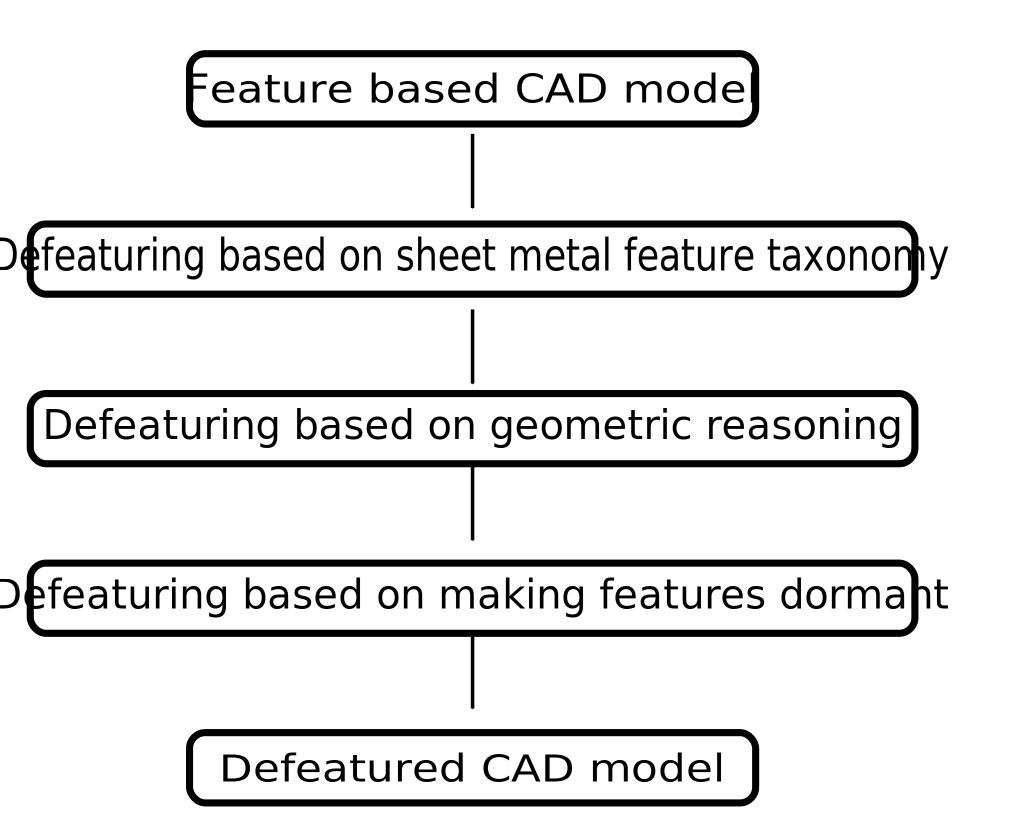
\includegraphics[width=0.5\linewidth]{images/SystemArchitectureDefeat_4.pdf}
		\caption{Overall Defeaturing Approach}
		\label{fig:defeaturing:OverallDefeaturingProcess}
	\end{figure}
	
%%\bigskip

 Figure~\ref{fig:defeaturing:OverallDefeaturingProcess} shows \added{phase-wise processing of the input sheet metal feature based CAD model by these criteria. Essentially these criteria apply various rules pertaining to application context, geometric reasoning and negative features, respectively. These rules are applied to identify the criticality of the features in the CAD model in the context of midsurface generation and attempts are made to remove not-so-relevant features from it. A threshold value is computed and provided to the overall approach. It denotes the ``size'' below which a feature is considered as irrelevant. The process thus simplifies the CAD model by defeaturing it while maintaining the gross shape intact. The phases of the proposed defeaturing process are explained below.}
	
\todo{Review comment: Directly start with the next section. [DONE]}
	
	\begin{itemize}
	[noitemsep,topsep=2pt,parsep=2pt,partopsep=2pt,leftmargin=*]
	\item \textbf{Phase I - Sheet Metal Taxonomy based}: The sheet metal CAD model feature tree is traversed and the candidate features for suppression are identified based on criteria based on the newly proposed sheet metal features taxonomy. For other domains or applications, this phase can be customized by employing application context specific taxonomies.
	
	\item \textbf{Phase II - Remnant Features}: This phase is generic and starts with the final Brep for identifying the remnant portions of the features. Those whose sizes are below the threshold are identified for suppression. One can customize the threshold based on engineering judgment appropriately.
	
	\item \textbf{Phase III - Dormant Bodies}: In this phase all ``negative'' features, even though they are relevant and thus have not been identified by the above two phases, are selected for removal, temporarily. Before removal, their feature bodies are cached/stored and are later used for re-applying on the output midsurface. 
	\end{itemize}
	

In the system implementing the proposed approach, it is important to note that, during defeaturing, even though the irrelevant features are said to be removed, they are discarded only temporarily and are not deleted permanently so that, in case of failure, they can be brought back and the original input CAD model to that stage can be restored.
 
%%%\begin{figure}[!ht]
%%%\RawFloats
%%\begin{minipage}[c]{0.95\linewidth}
%%    \begin{minipage}[c]{0.53\linewidth}
%%	\begin{itemize}
%%	[noitemsep,topsep=2pt,parsep=2pt,partopsep=2pt,leftmargin=*]
%%	\item \textbf{Phase I - Sheet Metal Taxonomy based}: The sheet metal CAD model feature tree is traversed and the candidate features for suppression are identified based on criteria based on the newly proposed sheet metal features taxonomy. For other domains or applications, this phase can be customized by employing application context specific taxonomies.
%%	
%%	\item \textbf{Phase II - Remnant Features}: This phase is gemeric and starts with the final Brep for identifying the remnant portions of the features. Those whose sizes are below the threshold are identified for suppression. One can customize the threshold based on engineering judgment appropriately.
%%	\end{itemize}
%%    \end{minipage}
%%    \hfill
%%    \begin{minipage}[c]{0.4\linewidth}
%%        \centering
%%        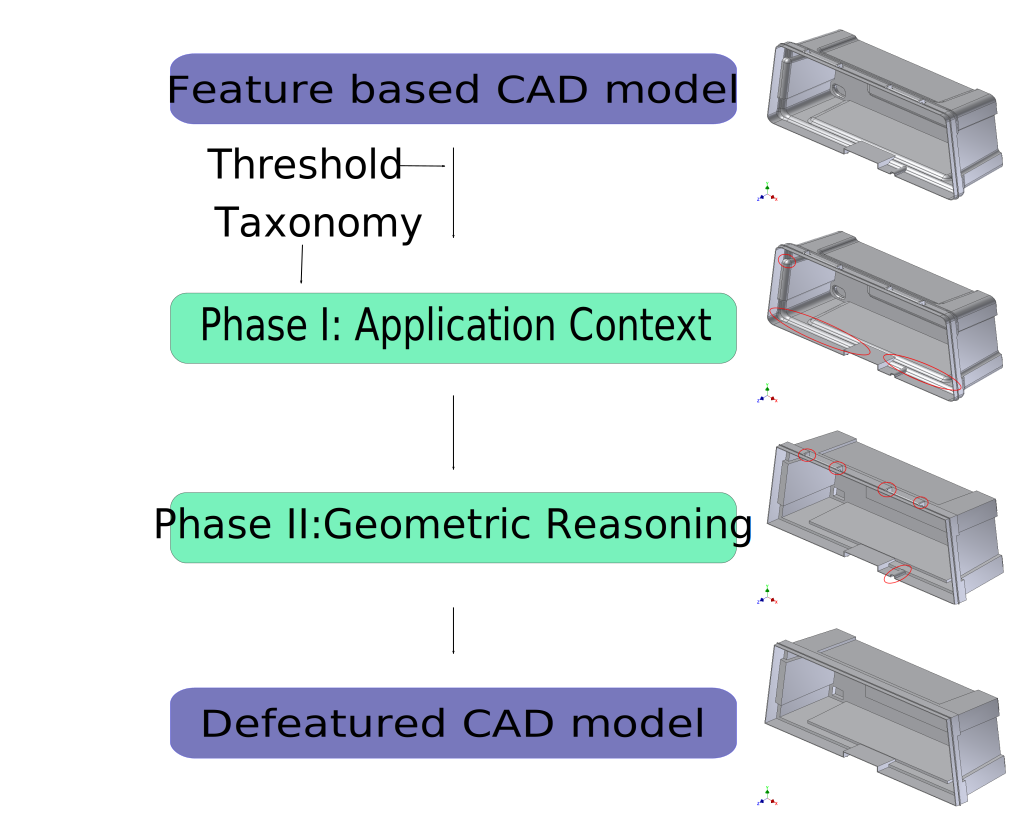
\includegraphics[width=\linewidth]{images/SystemArchitectureDefeat_1}
%%	 \captionof{figure}{Overall Process}
%%        	\label{fig:defeaturing:OverallDefeaturingProcess}           
%%    \end{minipage}
%%
%%\end{minipage}    
%%%\end{figure}

%The combined method (Phase I \& II) is called as ``\textbf{Smarf}'' (\textbf{S}heet \textbf{M}etal and \textbf{R}emnant \textbf{F}eatures). 
Following sections present the algorithms for these phases in details.


\section{Defeaturing Based on Sheet Metal Features \mbox{Taxonomy}}\label{sec:defeaturing:phase1}

CAD model under consideration is built by a number of sheet metal features such as Wall, Flange, Bend, etc. and are represented as a feature tree. This feature tree is traversed and the candidate features for removal are identified based on a criteria using the newly proposed sheet metal features taxonomy.

Figure ~\ref{fig:defeaturing:tax_sm} shows the proposed taxonomy which classifies sheet metal features and suggests their relevance with respect to maintaining the gross shape. In comparison with the other sheet metal features classifications, such as for features recognition~\cite{Gupta2013, Gupta2013a} and process planning~\cite{Kannan2009}, the proposed taxonomy is \replaced{different in a way that the classification is done based on the criticality of a particular feature to the gross shape.}{a novel one since the application context itself is different, and i.e. of finding the gross shape.}
%
%Sheet Metal parts are built using generic solid modeling features as well as some specialized sheet metal features. 
%
\subsection{Sheet Metal Features Taxonomy}\label{sec:defeaturing:phase11}

A thorough analysis of the inputs from various surveys with engineers and experts in the field to gauge relevance of sheet metal features with respect to the gross shape.  Proposed  taxonomy (Figure ~\ref{fig:defeaturing:tax_sm}) is the result of this analysis.

Taxonomy is represented by ``vocabulary'' and ``structure''~\cite{Tessier2011}. It is a scheme to represent and classify features for a particular purpose~\cite{Dartigues2005}.  Figure ~\ref{fig:defeaturing:tax_sm} shows the classification of sheet metal features for the purpose of computing gross shape.


%%\bigskip

%\begin{minipage}[c]{\linewidth}
\begin{center}
\begin{figure} [!h]
\dirtree{%
.1 Sheet Metal Features.
.2 Primary Features.
.3 Face-Wall   \adjustbox{valign=t}{\includegraphics[scale=0.65]{images/InventorWall.png}}.
.3 Flange  \quad \adjustbox{valign=t}{\includegraphics[scale=0.65]{images/InventorFlange.png}}.
.3 Bend   \qquad \adjustbox{valign=t}{\includegraphics[scale=0.65]{images/InventorBend.png}}.
%.3 Loft Flange  \qquad \adjustbox{valign=t}{\includegraphics[scale=0.65]{images/InventorLoftedFlange.png}}.
%.3 Rib \quad \quad  \adjustbox{valign=t}{\includegraphics[height=0.11\linewidth]{images/Feature_Rib.png}}.
.2 Secondary Features.
.3 Stamping  \quad \adjustbox{valign=t}{\includegraphics[scale=0.65]{images/InventorStamping.png}}.
.3 Cutout  \qquad \adjustbox{valign=t}{\includegraphics[scale=0.65]{images/InventorCutout.png}}.
%.3 Fold  \qquad \adjustbox{valign=t}{\includegraphics[scale=0.65]{images/InventorFold.png}}.
%.3 Roll  \qquad \adjustbox{valign=t}{\includegraphics[scale=0.65]{images/InventorRoll.png}}.
.3 Emboss \qquad \adjustbox{valign=t}{\includegraphics[scale=0.65]{images/InventorEmboss.png}}.
%.3 Hem   \quad \qquad \adjustbox{valign=t}{\includegraphics[scale=0.65]{images/InventorHem.png}}.
%.3 Grill \qquad \adjustbox{valign=t}{\includegraphics[scale=0.65]{images/InventorGrill.png}}.
.2 Tertiary Features.
%.3 Chamfer \qquad \adjustbox{valign=t}{\includegraphics[scale=0.65]{images/InventorChamfer.png}}.
%.3 Round  \qquad \adjustbox{valign=t}{\includegraphics[scale=0.65]{images/InventorRound.png}}.
%.3 Thread \qquad \adjustbox{valign=t}{\includegraphics[scale=0.65]{images/InventorThread.png}}.
.3 Lip \qquad \adjustbox{valign=t}{\includegraphics[scale=0.65]{images/InventorLip.png}}.
.3 Rest \qquad \adjustbox{valign=t}{\includegraphics[scale=0.65]{images/InventorRest.png}}.
%.2 Connecting Features.
%.3 Bend   \qquad \adjustbox{valign=t}{\includegraphics[scale=0.65]{images/InventorBend.png}}.
.2 Features Groups.
.3 Mirror \quad  \quad \adjustbox{valign=t}{\includegraphics[scale=0.65]{images/InventorMirror.png}}.
%.3 RectPattern \quad  \adjustbox{valign=t}{\includegraphics[scale=0.65]{images/InventorRectPattern.png}}.
.3 Pattern\quad  \adjustbox{valign=t}{\includegraphics[scale=0.65]{images/InventorCircPattern.png}}.
}
\caption{Sheet Metal Features Taxonomy (Icons source: Autodesk Inventor~\cite{Inventor2014Help})}\label{fig:defeaturing:tax_sm}
\end{figure}
\end{center}

%%\bigskip

%\begin{tabular}[h]{@{} p{0.45\linewidth}  p{0.45\linewidth}@{}} 
%%\begin{minipage}[c]{0.98\linewidth}
%%\begin{minipage}[t]{0.5\linewidth}
\begin{itemize}
[noitemsep,topsep=2pt,parsep=2pt,partopsep=2pt, leftmargin=*]
\item \textbf{Primary Features}: These features mainly contribute to the gross shape. Examples are  Face-Wall, Flange, Bend, etc.
%	\begin{itemize} [noitemsep,topsep=2pt,parsep=2pt,partopsep=2pt]
%	\item Face-Wall
%	\item Flange
%	\item Bend
%	\end{itemize}
\item \textbf{Secondary Features}: Relevance of these features is based on the relative size with respect to the size of the whole model. Examples are Stamping, Cutout, Emboss, etc.
%	\begin{itemize} [noitemsep,topsep=2pt,parsep=2pt,partopsep=2pt]
%	\item Stamping
%	\item Cutout
%	\item Emboss 
%	\end{itemize}
	
\item \textbf{Tertiary Features}: These features are irrelevant to the gross shape irrespective of their size relative to the size of the whole model. Examples are Lip, Rest, etc.
%	\begin{itemize} [noitemsep,topsep=2pt,parsep=2pt,partopsep=2pt]
%	\item Lip
%	\item Rest 
%	\end{itemize}
	
%\item \textbf{Connecting Features}: These are not suppressed irrespective of their sizes, as removing them, will create gaps between the sub-shapes of the original part. Lacking these would create gaps, so these are retained irrespective of their relative size, small or large.
%Example is:
%	\begin{itemize} [noitemsep,topsep=2pt,parsep=2pt,partopsep=2pt]
%	\item Bend
%	\end{itemize}
		
\item \textbf{Feature Groups}: These are feature collections. Their relevance is assessed as a collection, similar to the secondary features. Examples are Mirror, Patterns, etc.
%\begin{itemize} [noitemsep,topsep=2pt,parsep=2pt,partopsep=2pt]
%	\item Mirror
%	\item Patterns
%	\end{itemize}
\end{itemize}


		
%
%\begin{minipage}[t]{0.4\linewidth}
%		\includegraphics[width=\linewidth]{images/SheetMetal_taxonomy_2.pdf}
%		\captionof{figure}{Examples of classified types}
%		\label{fig:defeaturing:classification}
%\end{minipage}
%\end{minipage}    


Figure~\ref{fig:defeaturing:tax_sm} shows the proposed taxonomy classifying sheet metal features into categories such as Primary features, Secondary features, Tertiary features and Feature groups, based on their sheet metal domain specific characteristics. For defeaturing, each feature category undergoes its own rule for eligibility for removal during defeaturing process. Those rules are elaborated in detail in Section~\ref{sec:defeaturing:taxonomy}.

%%\bigskip

	\begin{figure} [!h]
		\centering
		\includegraphics[width=0.62\linewidth]{images/SheetMetal_taxonomy_3.pdf}
		\caption{Sheet Metal Features Based on Proposed Taxonomy}
		\label{fig:defeaturing:classification}
	\end{figure}
	
%%\bigskip

Figure~\ref{fig:defeaturing:classification} shows example part with various sheet metal features classified as per the proposed taxonomy. %%Following section details out the defeaturing process using the same classification.

\todo{Review comments: Logic of dormant feature needs to be clearly explained (in the algorithm) Why it is appearing here? [IT HAS BEEN MOVED TO ITS OWN SECTION LATER]}

\todo{Review Comments: Explain these steps with figure. [DONE]. Give figures for what is resultant model after processing primary then model after processing secondary and then tertiary. [IMPLEMENTATION IS DONE IN A SINGLE LOOP. WILL NEED TO RE-FACTOR SO THAT SEPARATE OUTPUTS CAN BE COLLECTED. WILL TRY THIS LATER]}

\subsection{Defeaturing Algorithm Based on Sheet Metal Features \mbox{Taxonomy}} \label{sec:defeaturing:taxonomy}

This subsection details the steps used to identify the removable sheet metal features based on the taxonomy proposed in Section~\ref{sec:defeaturing:phase11}. 
\todo{Review comment: What is threshold? Who defines it, what is the typical value you have found after experimenting? [ADDED EXPLANATION]}
Threshold value is computed based on the experimentations done~\cite{YogeshCADandA2016} to assess the effect of different threshold values on the quality of resultant midsurface output. Parameter $D$, which is used as a size criteria for deciding irrelevance of a feature, is defined as threshold \%age ($p$) of the size of the CAD model. Size of the CAD model can be defined in multiple ways, such as, size of Bounding Box, volume, etc. Bounding box as a measure of size, is quick to compute but not accurate. Volume is more accurate than Bounding box but is compute intensive, especially for Brep based CAD model, where the model is composed of faces. Sum of areas of the faces is both, reasonably accurate and easier to compute the size. Thus the present research measures size of the model as sum of the areas of all the faces. The \%age value for threshold is typically based on expertize, application context and engineering judgment. Various experiments were conduced to correlate effect of \%age value of threshold on the gross shapes. Table \ref{tbl:litsurvey:defeatmids} summarizes the results and more details are presented in Appendix~\ref{appendix:threshold}. Based on those experiments typical threshold values used in the present research work are 5-10\%.

Defeaturing rules based on sheet metal features taxonomy are enumerated below:
\begin{enumerate}
[noitemsep,topsep=2pt,parsep=2pt,partopsep=2pt, leftmargin=*]
\item \textbf{Primary Features}: Not removed as these features mainly contribute to the gross shape. Examples are  Face-Wall, Flange, Bend, etc.
%	\begin{itemize} [noitemsep,topsep=2pt,parsep=2pt,partopsep=2pt]
%	\item Face-Wall
%	\item Flange
%	\item Bend
%	\end{itemize}
\item \textbf{Secondary Features}: Are removed based on the relative size with respect to the size of the whole model. Features smaller than the threshold are removed, whereas bigger ones are retained.
%	\begin{itemize} [noitemsep,topsep=2pt,parsep=2pt,partopsep=2pt]
%	\item Stamping
%	\item Cutout
%	\item Emboss 
%	\end{itemize}
	
\item \textbf{Tertiary Features}: Are removed irrespective of their size relative to the size of the whole model. 
%	\begin{itemize} [noitemsep,topsep=2pt,parsep=2pt,partopsep=2pt]
%	\item Lip
%	\item Rest 
%	\end{itemize}
	
%\item \textbf{Connecting Features}: These are not suppressed irrespective of their sizes, as removing them, will create gaps between the sub-shapes of the original part. Lacking these would create gaps, so these are retained irrespective of their relative size, small or large.
%Example is:
%	\begin{itemize} [noitemsep,topsep=2pt,parsep=2pt,partopsep=2pt]
%	\item Bend
%	\end{itemize}
		
\item \textbf{Feature Groups}: Are removed based on the collective relative size with respect to the size of the whole model. 
%\begin{itemize} [noitemsep,topsep=2pt,parsep=2pt,partopsep=2pt]
%	\item Mirror
%	\item Patterns
%	\end{itemize}
\end{enumerate}

 	\begin{figure} [!h]
		\centering
		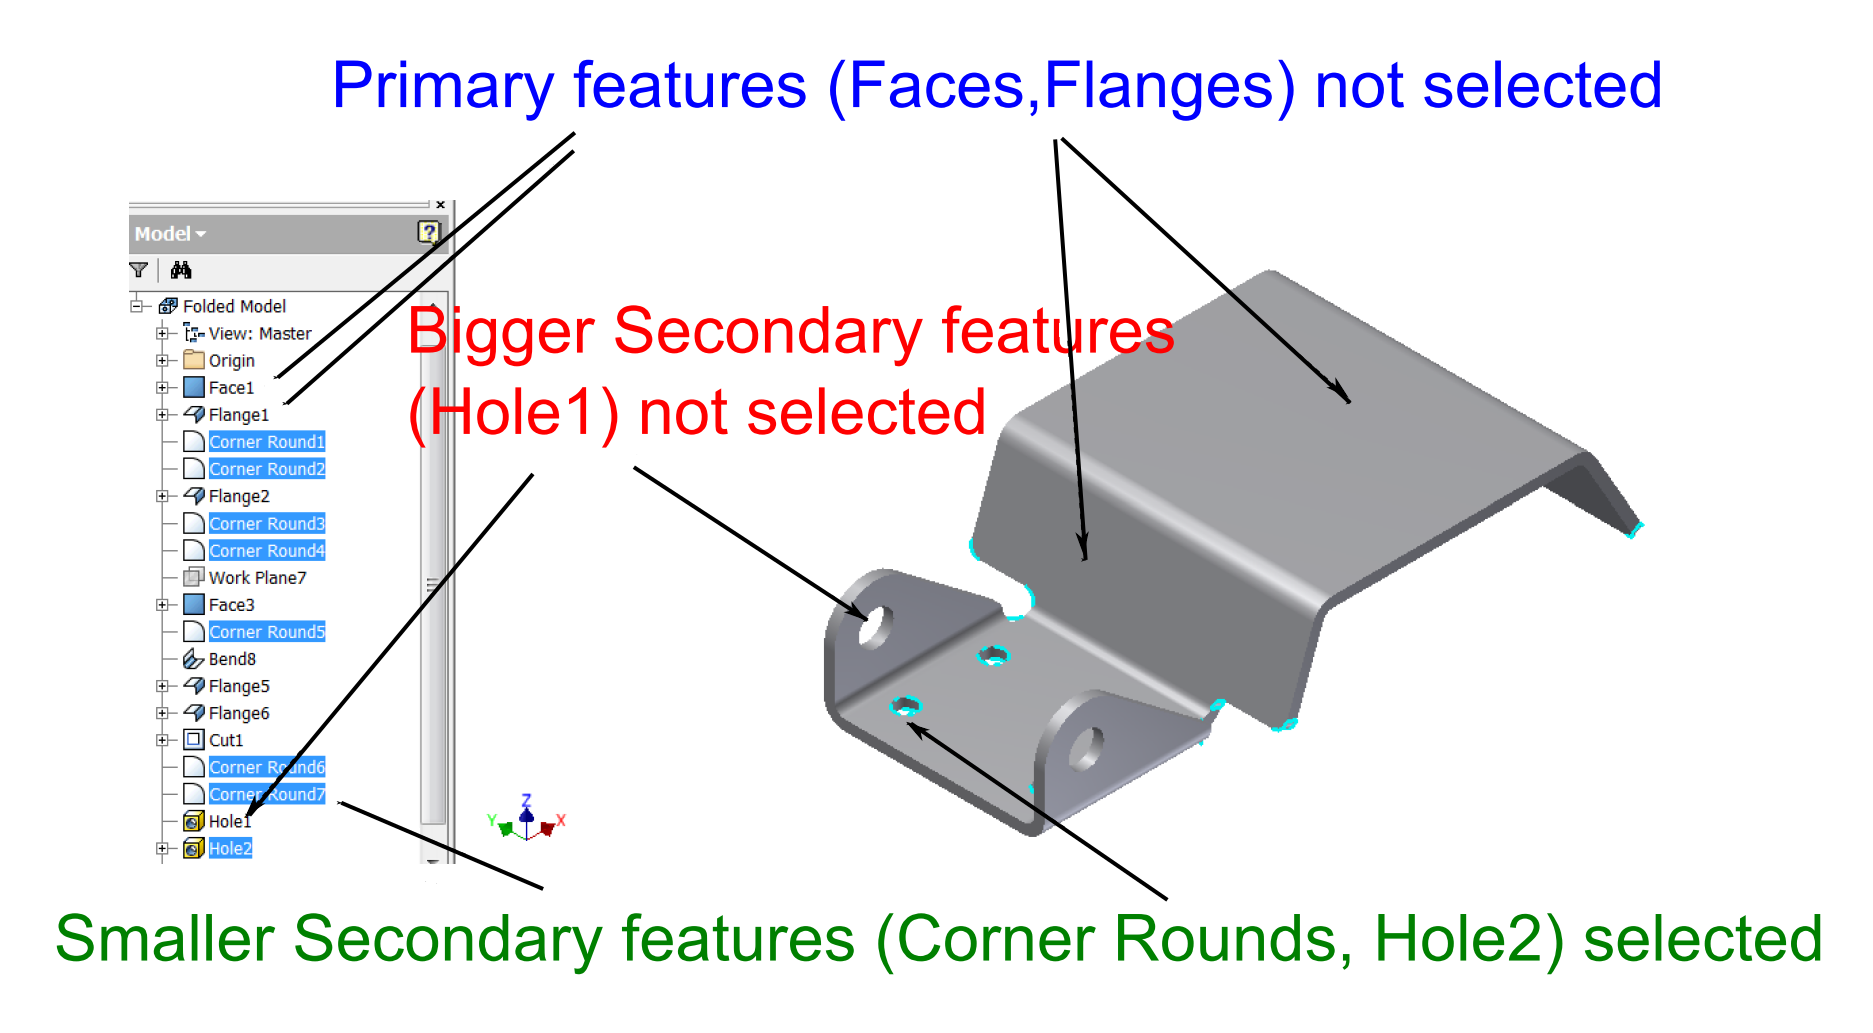
\includegraphics[width=0.62\linewidth]{images/SheetMetal_Ph1_Selection_Annotated_1.pdf}
		\caption{Defeaturing Based on Proposed Taxonomy }\label{fig:defeaturing:actions}
	\end{figure}
	
Figure~\ref{fig:defeaturing:actions} shows an example sheet metal part CAD model, with taxonomy based features categories shown, along with their defeaturing rules. Primary features such as Walls (Faces), Flanges are not removed. Secondary features whose face-size is less than the threshold are removed, but the larger ones are retained. With threshold as 5 \%, holes smaller than 5 \% of the model faces area, such as Hole2 and CornerRounds are selected but not the bigger holes such as Hole1.
 
%%\bigskip
 
%\subsubsection{Algorithm to identify candidate features for de-featuring based on Sheet Metal feature taxonomy:}
\begin{algorithm}[H]
	\caption{Phase I: Defeaturing Sheet Metal Features}
	\label{alg:defeaturing:phase1}
	\begin{algorithmic}[1]
		\REQUIRE A Sheet Metal FCAD model with access to the feature tree
		
%		\WHILE{$nextFace() != null$}
%			\STATE $F_i = currentFace()$
%			\STATE $Area_{face} \quad += F_i \rightarrow area()$
%		\ENDWHILE		
		\STATE $p = getPreDefinedThreshold()$
		\STATE $Area = sumAllFaceAreas()$
		\STATE $D = \frac{p}{100} \times Area$
		\WHILE{$f_i = currentFeature() != null$}
			\IF {$f_i \rightarrow isPrimaryFeature()$}
				\STATE continue
			\ELSIF {$f_i \rightarrow isTertiaryFeature()$}
				\STATE $sl \rightarrow add(f_i)$
			\ELSIF {$f_i \rightarrow isGroupFeature()$}
			  	\IF {$  f_i \rightarrow combinedArea() < D$}
			  		\STATE $sl \rightarrow add(f_i)$
				\ENDIF
			\ELSE
			  	\IF {$f_i \rightarrow area()  < D$}
			  		\STATE $sl \rightarrow add(f_i)$
%				\ELSIF  {$f_i \rightarrow isNegativeFeature()$}
%					\STATE $sl \rightarrow add(f_i)$ //Dormant feature
				\ENDIF				
			\ENDIF
		\ENDWHILE
		\STATE  $sl \rightarrow removeAll()$
		\STATE  $rebuildModel()$
	\end{algorithmic}
\end{algorithm}

%%\bigskip

Following are the steps taken for defeaturing CAD model based on sheet metal features taxonomy. Algorithm~\ref{alg:defeaturing:phase1} presents the same in pseudo-code form.

\begin{enumerate}
[noitemsep,topsep=2pt,parsep=2pt,partopsep=2pt]
\item The threshold \%age value is chosen. The threshold size is the threshold percentage times of the size of the model. The size of the model  is computed as the total of areas of all faces of the model. It is denoted as ``face-size'' of the model. Similarly, size of the feature is denoted as ``face-size of the feature'' and is the sum of area of the faces of the particular feature (Algorithm~\ref{alg:defeaturing:phase1}: lines 1-3).
\item The model feature tree is traversed and the current feature is applied with the defeaturing rules based on the newly proposed taxonomy (Figure~\ref{fig:defeaturing:tax_sm}, Figure~\ref{fig:defeaturing:actions}) (Algorithm~\ref{alg:defeaturing:phase1}: loop 4 to 18). 
\item The Primary features are not selected for removal so get skipped and do not get added to the removable-features list  (Algorithm~\ref{alg:defeaturing:phase1}: lines 5-6).
%\item The features are selected for removal based on the rules  as detailed out in section~\ref{sec:defeaturing:phase11} based on the newly proposed taxonomy (Figure~\ref{fig:defeaturing:tax_sm}). 
\item If the current feature is a ``Tertiary'' feature, then it is added directly to the removable-features list (Algorithm~\ref{alg:defeaturing:phase1}: lines 7-8).
\item If the current feature is a ``Group'' feature, then it's total face-size of the constituent features is checked against the threshold and if it is less then it is added to the removable-features list (Algorithm~\ref{alg:defeaturing:phase1}: lines 9-12).
\item If the current feature is a ``Secondary'' feature, then it's face-size checked against the threshold and if it is less then the feature is added to the removable-features list  (Algorithm~\ref{alg:defeaturing:phase1}: lines 14-16). 

\item Once all the features in the model are traversed, the features in the removable-features list are removed and the model is regenerated (Algorithm~\ref{alg:defeaturing:phase1}: lines 19-20).
%\item The `candidates list' is presented to the user for verification and changes, if necessary. 
%\item Features in the `candidates list' are removed.
%\item The model is regenerated and Defeaturing Effectiveness is computed using Eqn.~\ref{eqn:defeaturing:effectiveness}
%%
%%\item A list  ({\bf $sl$}) initialized to which the suppressible features are added. 
%%\item The model feature tree is traversed and the candidate features for suppression are identified based on a set of heuristic criteria such as ``Primary features are not to be suppressed'', ``Secondary features, if small, are selected'' etc.  (Figure~\ref{fig:defeaturing:actions}).
%%\item The identified features are added to {\bf $sl$}.
%%\item If ``Dormant' processing option is selected, all the negative features, which otherwise would not have qualified for the suppression are selected for suppression and added to  {\bf $sl$} . The bodies associated with these features are computed and cached. These bodies are later used to pierce the resultant Midsurface (Section~\ref{sec:defeature:dormant})
%%\item The {\bf $sl$} is presented to the user for verification and changes, if necessary. 
%%\item Features in  {\bf $sl$} are suppressed.
%%\item The model is regenerated and Defeaturing Effectiveness is computed using Eqn.~\ref{eqn:defeaturing:effectiveness}
\end{enumerate}


%%%\bigskip

%\subsection{Observations}

\todo{Review comment: Instead of Observations section, continue the algorithm section elaborate it wrt example. [DONE]}

\todo{Review commment: Need to explain this figure. [DONE]}

\begin{minipage}[t]{\linewidth}
\begin{tabular}[!h]{@{} p{0.3\linewidth} | p{0.3\linewidth} | p{0.3\linewidth}@{}} \toprule

\textbf{Input to Phase I} & \textbf{Detected Features} & \textbf{Output of Phase I} \\ \midrule

\includegraphics[width=0.92\linewidth]{images/DefeatPhase_I_t1} &
\includegraphics[width=0.98\linewidth]{images/DefeatPhase_I_t2} &
\includegraphics[width=0.99\linewidth]{images/DefeatPhase_I_t3} \\ \midrule

\includegraphics[width=0.98\linewidth]{images/DefeatPhase_I_1} &
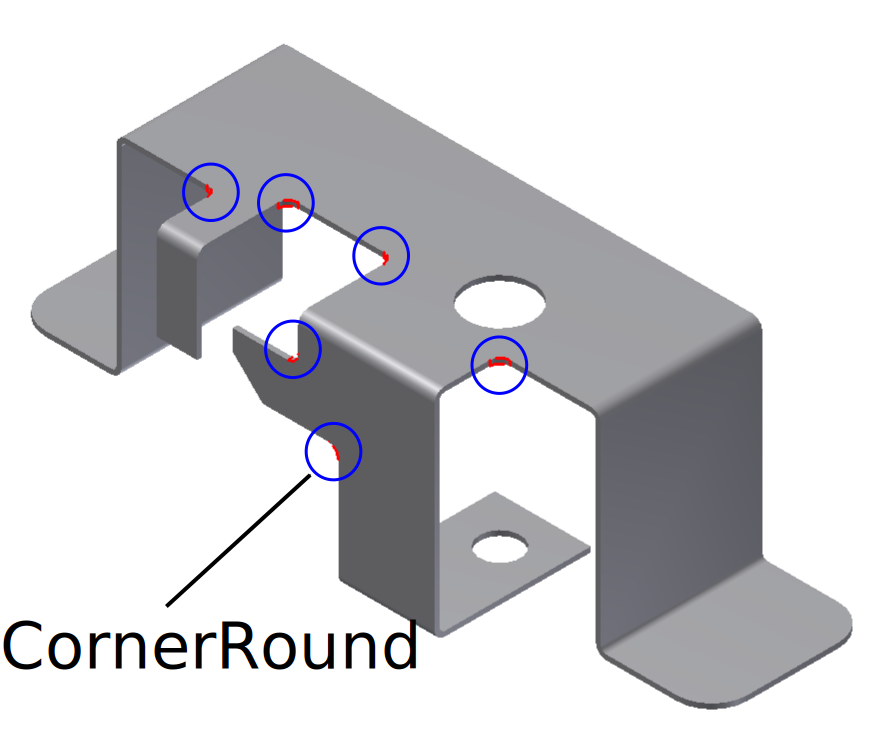
\includegraphics[width=0.98\linewidth]{images/DefeatPhase_I_2_new_nolables.pdf} &
\includegraphics[width=0.98\linewidth]{images/DefeatPhase_I_3} \\ \bottomrule

\end{tabular}
\captionof{figure}{Phase I: Defeaturing Based on Feature Taxonomy and Size Threshold Approach}\label{fig:defeaturing:phaseI}
\end{minipage}

Figure~\ref{fig:defeaturing:phaseI} shows the process pictorially. The first column, called ``Input to Phase I'' shows input sheet metal features CAD model of a bracket part, along with its feature tree. The second column, called ``Detected Features'' shows the candidate features selected, such as `Corner Round1', on the model as well as in the feature tree, based on the steps mentioned above (also mentioned in Algorithm~\ref{alg:defeaturing:phase1}).  The third column shows the output of Phase I, showing the model with candidate features removed.

%%\bigskip




%%\bigskip

%\vspace{-3mm}

\todo{Review comment: At the end state what you conclude with this phase I processing. [DONE]}

With the Phase I over, sheet metal domain specific defeaturing is complete. This phase can be further enhanced by either customizing the threshold and/or by incorporating more features in the taxonomy based on further surveys and experimentations. It can be customized further, for different application domains, such as Injection Molding, by incorporating taxonomy specific to those domain. 

Following section details out the Phase II, i.e. defeaturing process based on geometric reasoning.

 %\vspace{-5mm}
 
\section{Defeaturing Based on Geometric Reasoning of CAD Model Features} \label{sec:defeaturing:phase2}

\todo{Review comment: Change title to Geometric reasoning of model features. [DONE. ADDED `CAD']}

The sheet metal feature based CAD models used in the present research work are built using `design-by-features' approach. At each feature step, the feature parameters first generate a feature primitive solid, known as ``tool-body''. Boolean operation is  performed between operands: the existing model at that stage and the tool body. During this operation, some portion of the tool-body-portion gets consumed within the existing model and the remaining portion of the tool body appears as a newly added feature in the CAD model. 


%%\bigskip

 	\begin{figure} [!h]
		\centering

\includegraphics[width=0.62\linewidth,valign=t]{images/Solid_Simple_SmallProtrusion_labels_2.pdf}
		\caption{Remnant and Consumed Portions} \label{fig_remnant}
	\end{figure}
	
%%\bigskip

Figure ~\ref{fig_remnant} shows boolean operation between the existing CAD model denoted by  $M$ and the tool body of feature $f_2$. Some portion of the tool body gets consumed and is merged with the model whereas some portion remains outside. The portion remaining outside is referred as ``remnant feature'' portion. This phase involves the geometric reasoning to identify remnant feature portions on the input Brep CAD model.

Past attempts such as by Russ~\cite{Russ2012}, used full feature tool-body to determine the candidature for removal during defeaturing. This obviously gives incorrect results as the CAD model actually retains only the remnant portion of the feature. Size of only remnant portion should be considered for deciding the candidature for removal. Thus the present research  uses the size of the remnant portion for deciding removal of a feature and the algorithm to do this is presented below.


\subsection{Defeaturing Algorithm Based on Remnant Feature Portions}

%%In the feature based design paradigm, the CAD model is built step-by-step using features at each step.  At $j^{th}$ feature ($f_j$), the model built till then is referred as $M_{j-1}$.   Feature parameters are used to compute the ``canonical'' (tool-body) volume first, which is then booleaned to the model built till then. $V_j = volume (f_j)$. $V_j$ is the feature/canonical/tool-body volume of the feature $f_j$. $M_j = M_{j-1} \oplus V_j$. The model moves to the next state $M_j$ by boolean of existing state $M_{j-1}$ with the feature volume $f_j$ i.e. $V_j$.  During this operation, some portion of the canonical volume may get consumed, leaving behind the remaining (remnant) volume in the final solid  (Fig.~\ref{fig_remnant}). $V_j = R_{j} \cup C_j$. Some portion of $V_j$ gets consumed ($C_j$) and some remains ($R_j$). (Fig.~\ref{fig_remnant}). $M_j = M_{j-1} \cup  R_j$ and thus $R_j = M_{j} -   M_{j -1}$ is the remnant feature volume ~\cite{Lee2005}.

%%\begin{figure}[!htb]
%%\centering
%% \includegraphics[width=0.35\linewidth]{images/Solid_Simple_SmallProtrusion.pdf} 
%% \caption{Remnant and Consumed portions of feature volume of  $f_2$}
%% \label{fig:defeaturing:remnant}
%%\end{figure}
%%  
%%Identification of suppressible features based on the feature volume computed from the full feature parameters yield incorrect results as the final shape may not retain the full feature volume. So, this work has devised a novel method  (Algorithm~\ref{alg:defeaturing:phase2}) to find the size of remnant feature volume to be used for deciding the suppressibility  (Fig.~\ref{fig:defeaturing:phaseII}) of the features. This phase starts with the final Brep for identifying the remnant portions of the features. This computation, being geometric in nature, can be generic to many applications, with an option to customize the threshold based on engineering judgment specific to the given application.
%%
%%\subsection{Approach}
%%
The input to this phase is the output CAD model from Phase I. In contrast to phase I, this phase does not involve traversal of the feature tree. Instead, it traverses faces of the final model i.e. the Brep model available at the end of the feature tree. As these faces have remained in the model till the end, they are termed as `remnant' faces. The Brep CAD solid model is termed as `final body'. Whenever a feature is added, it adds new faces to the existing Brep model. These new faces store information of the feature which created it, which is termed as the ``owner feature''. The owner feature information is stored on all faces of the Brep as attributes, typically referred as ``origination info''.

The intent of this phase is to group all the remnant faces belonging to a particular feature. This group is termed as `FaceGroup'. Then identify their respective feature owners, and decide their removability on the size of their remnant portions. The size of a FaceGroup can be calculated by various approaches like Influence Volume~\cite{SangHunLee2005} or the union of bounding-boxes, etc. The present work uses summation of the area of the remnant faces as the `Size' criterion and is called ``face-size''. The choice of area as the size criteria is based on ease of computability and reasonable accuracy to represent the remnant portion. 



Following steps present details of the algorithm used to identify remnant faces and thereby remnant features, to be removed based on the remnant portion of the tool body (Figure~\ref{fig_remnant}) (Algorithm~\ref{alg:defeaturing:phase2}).
\todo{Review comment: What is this (clusters table)? its unit, irs rationale, why you use this for what purpose, where are these in figure. [EXPLAINED HERE]}
\todo{Review comment: Give numbers to list items. [DONE]}
\todo{Review comment: A new term (FaceGroup) is coined here which is not explained here. [DONE]}

\begin{enumerate}
[noitemsep,topsep=2pt,parsep=2pt,partopsep=2pt]
\item Remnant faces of the final body are traversed. (Algorithm~\ref{alg:defeaturing:phase2}: loop 1 to 15).  
\item For each remnant face, its owner feature is retrieved (Algorithm~\ref{alg:defeaturing:phase2}: line 2).
\item Existing FaceGroups are searched for matching owner feature.
\item If a match exists, the face is added to that FaceGroup  (Algorithm~\ref{alg:defeaturing:phase2}: lines 4-8).
\item If a match is not found, then a new FaceGroup is created, the remnant face is added to it, it owner feature is set as the owner of the FaceGroup and this new FaceGroup gets appended to the list of FaceGroups  (Algorithm~\ref{alg:defeaturing:phase2}: lines 9-13).

\bigskip

\begin{minipage}{\linewidth}

\begin{minipage}[c]{0.48\linewidth}
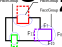
\includegraphics[width=0.8\linewidth,valign=t]{images/facegroups_1.pdf}
\captionof{figure}{FaceGroups} \label{fig_clusters}
\end{minipage}
%%\begin{figure}[!h]%[!h]
%%\centering     
%%\subfloat[Remnant and Consumed portions of $f_2$]{\label{fig_remnant}\includegraphics[width=0.5\linewidth,valign=t]{images/Solid_Simple_SmallProtrusion.pdf}} \quad
%%\subfloat[Formation of clusters]{\label{fig_clusters}\includegraphics[width=0.25\linewidth,valign=t]{images/clusters.pdf}}
%%\caption{Phase II: Remnant feature definition, Cluster approach} 
%%\label{fig:defeaturing:phaseII}
%%\end{figure}
\hfill
\begin{minipage}[c]{0.48\linewidth}
\captionof{table}{FaceGroups Details}
\label{tbl_clusters}
\begin{tabular}[h]{@{} p{0.3\linewidth} p{0.25\linewidth} p{0.25\linewidth}@{}} \toprule
\textbf{FaceGroup Id} & \textbf{Face-size ($mm^2$)}& \textbf{Owner Feature}\\ \midrule
FaceGroup$_1$ & 0.25 	&  Extrude$_2$\\
FaceGroup$_2$ & 0.25  & Extrude$_3$\\
FaceGroup$_3$ & 0.125 & Hole$_1$\\ \bottomrule
%$f_{10}, f_{12}, f_{15}, f_{14}$ 	& Cluster$_4$\\ \bottomrule
\end{tabular}
\end{minipage}
\end{minipage}
%%\bigskip

%%\bigskip

Figure~\ref{fig_clusters} shows a schematic of existing Brep CAD model with 3 features booleaned to it. Thick lines are used to represent the remnant faces whereas dotted lines are used to represent the consumed faces. FaceGroup1 and FaceGroup3 are depression features, i.e. negative features, whereas FaceGroup2 is a protrusion feature i.e. a positive feature. In FaceGroup2, $F_{11}$ is a consumed face whereas Faces $F_{10},F_8,F_7$ are the remnant faces. So, FaceGroup2 represents remnant portion of the owner feature Extrude$_3$.

%\item  FaceGroups are formed with same owning features as shown in Figure~\ref{fig_clusters}, where the dotted portions show the consumed feature portions and the circles show the remnant portions. 
\item Face-sizes of the FaceGroups are computed. Table~\ref{tbl_clusters} shows face-size (in $mm^2$) along with owner feature of each FaceGroup.
\item A FaceGroup is removed if its face-size is below the threshold value (Algorithm~\ref{alg:defeaturing:phase2}: lines 16-18). The threshold used is same as the one used in Algorithm~\ref{alg:defeaturing:phase1}: lines1-3.
%%\item The candidates list is presented to the user for verification and changes, if necessary. 
\item Once all the FaceGroups are assessed, removable-features are removed from the feature tree and the model is rebuilt (Algorithm~\ref{alg:defeaturing:phase1}: lines 20-21).
%%\item The model is regenerated and Defeaturing Effectiveness is computed using Eqn.~\ref{eqn:defeaturing:effectiveness}
\end{enumerate} 

\bigskip

\begin{algorithm}[H]
	\caption{Remnant Feature Method}
	\label{alg:defeaturing:phase2}
	\begin{algorithmic}[1]
		\REQUIRE A CAD model with access to the feature tree. 
		\WHILE{$F_i = currentFace() != null$}  
			\STATE $feat = F_i \rightarrow owingFeature()$
			\STATE $addedFlag = false$
			\WHILE {$cl_j = currentFaceGroup() != null$}
				\IF {$cl_j \rightarrow owingFeature() == feat$}
					\STATE  $cl_j \rightarrow add(F_i)$, $addedFlag = true$
				\ENDIF
			\ENDWHILE
			\IF {$addedFlag == false$}
				\STATE  $cl_n = newFaceGroup()$
				\STATE  $cl_n \rightarrow owingFeature() = feat$
				\STATE  $cl_n \rightarrow add(f_i)$
			\ENDIF
		\ENDWHILE
		\WHILE {$cl_k = currentFaceGroup() != null$}
			\IF {$cl_k \rightarrow calculateSize() < D$} %\hspace{40mm} // Threshold D defined in Alg~\ref{alg1}
				\STATE   $sl \rightarrow add(cl_k)$
			\ENDIF			
		\ENDWHILE
		\STATE  $sl \rightarrow removeAll()$
		\STATE  $rebuildModel()$
	\end{algorithmic}
\end{algorithm}


\bigskip

Figure~\ref{fig:defeaturing:phaseII} shows the process pictorially. The first column, called ``Input to Phase II'' shows the sheet metal features CAD model of a bracket part partially defeatured in the Phase I,  along with its feature tree. The second column, called ``Detected Features'' shows the candidate features selected, such as Holes, on the model as well as in the feature tree, based on Algorithm~\ref{alg:defeaturing:phase2}. The Hole is made by cutting a cylinder like tool body. This tool body's dimensions are big enough to disqualify it from removal. But the remnant faces in the model are small enough to qualify this feature for removal. Third column shows the output of Phase II, showing the model with candidate features removed.
%\subsection{Observations}

\bigskip

\begin{minipage}[t]{\linewidth}
\begin{tabular}[h]{@{} p{0.3\linewidth} | p{0.3\linewidth} |  p{0.3\linewidth}@{}} \toprule

\textbf{Input to Phase II} & \textbf{Detected Features} & \textbf{Output of Phase II} \\ \midrule

\includegraphics[width=0.92\linewidth]{images/DefeatPhase_II_t1} &
\includegraphics[width=0.98\linewidth]{images/DefeatPhase_II_t2} &
\includegraphics[width=0.99\linewidth]{images/DefeatPhase_II_t3} \\ \midrule

\includegraphics[width=0.98\linewidth]{images/DefeatPhase_I_3} &
\includegraphics[width=0.92\linewidth]{images/DefeatPhase_II_2_new_wlables.pdf} &
\includegraphics[width=0.98\linewidth]{images/DefeatPhase_II_3} \\ \bottomrule

\end{tabular}
\captionof{figure}{Phase II: Defeaturing Based on Remnant Feature Approach}\label{fig:defeaturing:phaseII}
\end{minipage}

\todo{Review comments: Drop this (observations) section. Continue previous section with elaborate explanation wrt figure. [DONE. ALSO: NEED TO IMPROVE FIGURE AND COMMENTARY. CURRENTLY FUZZY]}






\todo{Review comments: change column names. [THINKING OF ALTERNATIVES]}

%%\bigskip



%%\bigskip

After the first two phases, the given example of bracket model shows 50\% reduction in the number of features and 17\% reduction in the number of faces, at 5\% threshold value. The resulting gross shape has retained all important features necessary for the computation of a quality midsurface.

\section{Defeaturing Based on Dormant Feature Tool-bodies}\label{sec:defeature:dormant}

\todo{Review comment; Change title to bulk features. [NOT CHANGING THE TITLE AS OF NOW TO `DEFEATURING BASED ON BULK FEATURE REMOVAL' AS I AM NOT GETTING ITS MEANING. IN THE PARA, I AM TREATING `BULK' AS `LARGE'.]}

Bulk negative features, such as large Holes, Cutouts can be potentially problematic in further processes used in the midsurface computation, such as feature generalization (Chapter~\ref{ch:Abstraction}) and cellular decomposition (Chapter~\ref{ch:Midsurface}). But they can not be removed because they are necessary constituent of the gross shape. 

\todo{Review comment: First provide rationale as to why some features rather bulk in size need to be mad dormant rather than defeatured. [DONE]}

The results shown in Table~\ref{tbl:litsurvey:defeatmids} demonstrate that removal of negative features, even though they are relevant, can help computation of midsurface. But the drawback is, these features, being relevant would be missing on the midsurface. The present research work proposes to gain the computational advantage but at the same time does not want to loose the relevant features. This proposed approach is called as the Dormant Features approach. In this approach, relevant negative features are removed temporarily, but while doing so their feature bodies (called ``tool-bodies'') are preserved for later usage. After computing midsurface from such highly defeatured model, the preserved tool bodies are brought back and are re-applied on the midsurface. Thus, effect of those important, relevant negative features on midsurface is not lost. However temporary removal does substantially simplify the model which make midsurface computation quite convenient. Following section elaborates Phase III, the dormant features approach.


%\subsection{Approach}\label{sec:defeature:dormantapproach}
\subsection{Defeaturing Algorithm Based on Dormant Features}\label{sec:defeature:dormantalgo}

\todo{Review comment: What is the strategy to identity such features?. [ADDED]}

At this stage, Phases I and II are already over. All the small, irrelevant features are already removed. All the remaining features now, are the relevant features. These can include the negative features as well. In the steps mentioned below, in-spite of being relevant, the large negative features are temporarily removed, after storing their tool bodies. These bodies are kept dormant to be used later for piercing on the midsurface. Algorithm~\ref{alg:defeaturing:phase3} presents pseudo code of the approach and has been listed below: 

\bigskip


\begin{algorithm}[H]
	\caption{Phase III: Dormant Features Identification}
	\label{alg:defeaturing:phase3}
	\begin{algorithmic}[1]
		\REQUIRE A Sheet Metal FCAD model with access to the feature tree
		
%		\WHILE{$nextFace() != null$}
%			\STATE $F_i = currentFace()$
%			\STATE $Area_{face} \quad += F_i \rightarrow area()$
%		\ENDWHILE		
		\WHILE{$f_i = currentFeature() != null$}
			\IF {$f_i \rightarrow isNegativeFeature()$}
				\STATE $b_i = computeToolBody(f_i)$
				\STATE $bl \rightarrow add(b_i)$
				\STATE $sl \rightarrow add(f_i)$
			\ENDIF
		\ENDWHILE
		\STATE  $sl \rightarrow removeAll()$
		\STATE  $rebuildModel()$
	\end{algorithmic}
\end{algorithm}

\bigskip

\todo{Review comment: You are not giving any sense of being dormant here. [ADDED, BOTH, HERE AND IN ALGO]}

\begin{enumerate}
[noitemsep,topsep=2pt,parsep=2pt,partopsep=2pt]
\item The input CAD model feature tree is traversed (Algorithm~\ref{alg:defeaturing:phase3}: loop 1 to 7). 
\item  The current feature is tested if it is a negative feature, like Hole, Cutout, Extrude with subtractive boolean, etc. (Algorithm~\ref{alg:defeaturing:phase3} line: 2). 
\item The tool body is computed using its feature parameters (Algorithm~\ref{alg:defeaturing:phase3} line: 3). 
\item The tool-body is stored in a list (Algorithm~\ref{alg:defeaturing:phase3} line: 4). 
\item The current feature is added to list for removal (Algorithm~\ref{alg:defeaturing:phase3} line: 5). 
\item Once all the features in the feature tree are traversed, the features from candidate features list are removed and the CAD model is rebuilt (Algorithm~\ref{alg:defeaturing:phase3}: lines 8-9).
\end{enumerate}

%By the deferment of processing dormant features, generating midsurface patches gets simplified as these features are not present during their computation.  
\todo{Review comment: Clearly explain algorithm with figure. [IT SHOWS THE APPLICATION OF DORMANT AND NOT SELECTION. AM NEED TO REPLACE WITH A BETTER FIGURE, IF POSSIBLE]}


%%\bigskip




%%\bigskip
	
%\subsection{Observations}\label{sec:defeature:dormantobs}

%%%%\bigskip
%%
%% 	\begin{figure} [!h]
%%		\centering
%%\includegraphics[width=0.45\linewidth,valign=t]{images/dormant_labels.pdf}
%%		\caption{Re-application of the Dormant Feature Tool-body on Midsurface} \label{fig_dormant}
%%	\end{figure}
%%	
%%%%\bigskip

	\begin{figure}[h!]
	\centering 
	%\includegraphics[width=0.85\linewidth]{images/facepairing}
	\subfloat[Input CAD Model]{\label{fig:midsurfcelljoin:beforedomant}\includegraphics[width=0.5\linewidth,valign=t]{images/UBracket_part}} \hfill
	\subfloat[Semi-Final Midsurface]{\label{fig:midsurfcelljoin:semimids}\includegraphics[width=0.49\linewidth,valign=t]{images/MidsurfBracket}} \hfill
	\subfloat[Dormant Tool Bodies Re-application]{\label{fig:midsurfcelljoin:dormant}\includegraphics[width=0.49\linewidth,valign=t]{images/MidsurfDormantBodies_2}} \hfill
	\subfloat[Final Midsurface]{\label{fig:midsurfcelljoin:finalmids}\includegraphics[width=0.49\linewidth,valign=t]{images/MidsurfAfterDormant}}
	\caption{Re-application of the Dormant Feature Tool-bodies on Midsurface}
	\label{fig_dormant}
	\end{figure}
	
Figure~\ref{fig_dormant} shows reapplication i.e piercing of the dormant feature tool bodies. Figure~\ref{fig:midsurfcelljoin:beforedomant} depicts model before detection of the dormant features. Figure~\ref{fig:midsurfcelljoin:semimids} shows midsurface computed after removal of the dormant features. The cached dormant feature tool bodies are brought back and are re-applied on the midsurface, as shown in Figure~\ref{fig:midsurfcelljoin:dormant}. So, the presence of relevant negative features is made sure in the final midsurface as depicted in Figure~\ref{fig:midsurfcelljoin:finalmids}. Thus ensuring faithful representation of all the prominent features on the midsurface. 
%
%\begin{minipage}{0.95\textwidth}
%\begin{minipage}[c]{0.42\linewidth}
%\includegraphics[width=0.75\linewidth,valign=t]{images/dormant}
%\captionof{figure}{Re-application of the Dormant Feature Tool-body on Midsurface} \label{fig_dormant}
%\end{minipage}
%\hfill
%\begin{minipage}[c]{0.56\linewidth}
%% (Refer example in Section~\ref{sec:results:computation} for more details).
%Stored dormant features' tool bodies are reapplied on the midsurface. More details at Figure~\ref{fig:midsurfcelljoin:midsdorm}.
%\end{minipage}
%
%\end{minipage}

\todo{Review comment: Provide  a paragraph of your comment on what is outcome of these three phases. [DONE]}

Table \ref{tbl:defeaturing:benchmarking} shows a brief comparison of the present research work, as implemented in \mysystemname, with the other defeaturing approaches, such as, by Brian Russ~\cite{Russ2012},  Sungchan Kim et. al~\cite{Kim2005} and Sang Hun Lee~\cite{Lee2005}.

\bigskip
%------------------------------------------------------------------------------------
\begin{minipage}[t]{0.9\linewidth}
  \centering
   \captionof{table}{Comparison of the Present Research with Other Methods}
  \label{tbl:defeaturing:benchmarking}
%  \resizebox{\linewidth}{!}{ 
\begin{longtable}[htp]{@{} p{0.16\linewidth} |p{0.18\linewidth} | p{0.18\linewidth}| p{0.18\linewidth} |p{0.18\linewidth}@{}}
\toprule
\textbf{Methods} & \textbf{Russ~\cite{Russ2012}} &	\textbf{Kim~\cite{Kim2005}} &	\textbf{Lee~\cite{Lee2005}} & \textbf{\mysystemname}\\
\midrule
\textbf{Input} & Features	& Brep	& Features	& Features\\
\midrule
\textbf{Approach} & Suppresses if feature size is less than threshold.&
Wrap-around. Negative volumes removed totally. &
Feature volumes are reordered in sorted manner.&
Suppress based on taxonomy and remnant volumes.\\
\midrule
\textbf{Advantages} & Automatic identification of non-critical features &
 Does not need features; Works on Brep&
 Multiple defeaturing levels possible& More accurate criteria for defeaturing
\\
\midrule
\textbf{Limitations} & Limited to FEM as BC and Load path features are not suppressed. &
Concave edge filling creates odd shapes. Principal shape is lost. &
Due merged Cellular model, update capability is lost forever. &
Taxonomy needs to be updated for new features\\	
\bottomrule
\end{longtable}
%}

\end{minipage}


\bigskip

\added{The comparison indicates that the defeaturing approach presented in this chapter significantly reduces the number of faces in the CAD model thus simplifying it considerably for the purpose of midsurface computation. It, however, still ensures that the gross shape of the input CAD model is retained so that underlying design intent is not lost.}

In summary, Phase I removes features from the input CAD model based on the newly proposed sheet metal features taxonomy. The model gets further simplified in Phase II using remnant feature portions approach. Phase III simplifies the model further by completely removing all the negative features. After completion of all three phases of defeaturing the input sheet metal features CAD model is more or less reduced to its gross shape. This is optimum and effective level of defeaturing. Any further removal of the features will disturb the original gross shape intent.

Following section presents a newly proposed measure to assess the effectiveness of the defeaturing process.

\section{Effectiveness of Defeaturing}\label{sec:defeaturing:effectiveness}

\todo{Review comment: Not clear whether these are existing approaches. [THESE ARE EXISTING APPROACHES]}

Effectiveness of the defeaturing process is computed using a wide variety of methods\added{, such as quantitative reduction, MAT, Mesh based, etc.} They can be classified into input-based and output-based methods. In the input-based method, engineering judgment is used to set the initial defeaturing parameters, such as, size threshold, feature taxonomy, etc. and the output resulted is considered as the valid~\cite{MobleyCarrollCanann1998}. In the output-based method, some initial defeaturing parameters are set and the output is assessed against predefined benchmarks, such as, reduction in volume or number of faces or features, etc. The process is repeated till the benchmarks are  achieved. 

In the present research, the input-based method is used to assess the effectiveness of defeaturing. It is computed by measuring {\bf Percentage reduction in the number of faces}. Measurements are done before and after a particular defeaturing phase. More the percentage, more effective is the defeaturing process. A measure of reduction in number of features can also be used in place of faces to form another criterion for assessing the effectiveness. The present research work collects following parameters to compute the effectiveness:

\todo{Review comments: Rename Phase I, II. [RETAINED THESE NAMES, AS THEIR MEANING IS EXPLAINED IN PARAGRAPH ABOVE]}

	\begin{enumerate}
	[noitemsep,topsep=2pt,parsep=2pt,partopsep=2pt]
%	\item Total area of the Faces ($aF$)  ($mm^2$) 
%	\item Threshold size is some (say, 5 percent) of $aF$ ($sP$ $mm^2$)
	\item Total number of the faces in the original part ($nF$)
%	\item Number of sheet metal features suppressed in Phase I ($nS$)
	%\item Time spent in detecting the suppressible features in Phase I ($tS$ sec) 
%	\item Number of faces remaining in the model after Phase I ($mF$)
%	\item Number of \deleted{generic} features suppressed in Phase II ($nR$)
	%\item Time spent in detecting the suppressible features in Phase II ($tR$ sec)	
	\item Number of faces remaining in the model after defeaturing ($rF$)
	\item Defeaturing effectiveness ($pR$) (\%)
	\begin{equation}\label{eqn:defeaturing:effectiveness}  pR = (1 - \frac{rF}{nF}) \times 100\end{equation}
	\end{enumerate}

Defeaturing effectiveness ($pR$) gives quick idea of the order of magnitude of defeaturing.

Following section demonstrates efficacy of the proposed defeaturing approach by evaluating it against CAD model of a real-life test part.

\todo{[REMOVED OTHER METHODS. NOT VERY CONVINCING]}

%%Apart from $pR$, there could be some other and more involved criteria that can be used as follows:
%%	\begin{itemize}
%%	[noitemsep,topsep=2pt,parsep=2pt,partopsep=2pt]
%%	\item \textbf{Medial Axis Comparisons}: Medial Axis Transform (MAT~\cite{Ramanathan2004}) is a skeletal representation of a model. Model, with lots of details will typically generate MAT with branches at the location of details, whereas a simplified model, i.e. without numerous detauils, will not have branches at those locations. Figure~\ref{fig_matbranch} shows how MAT of a simple shape and a shape with extra detail differs. So, Comparison of MAT in case of model before and after defeaturing, by comparing branches can give idea about the effectiveness of the defeaturing process.
%%	
%%%%\bigskip
%%
%% 	\begin{figure} [!h]
%%		\centering
%%\includegraphics[width=0.55\linewidth,valign=t]{images/matbranch}
%%		\caption{Introduction of a detail adds a branch in MAT (Source~\cite{Chen1998})} \label{fig_matbranch}
%%	\end{figure}
%%	
%%%%\bigskip	
%%	
%%\todo{[REMOVED MESH COMPARISON. NOT VERY CONVINCING]}	
%%%	\item \textbf{Mesh}: Comparing faceted mesh generated by body defeatured by {\bf Smarf} with the mesh simplified by any benchmark mesh simplification methods can give the effectiveness measure.
%%	\item \textbf{Size}: Comparison of volume of the original and the defeatured model.
%%	\item \textbf{Shape deviation}: Using Part-Compare functionality, maximum deviation between the original and the defeatured, can be calculated. This deviation should be within predefined limits.
%%\end{itemize}



\todo{Review comment: Drop Implementation section. [DONE]}

%----------------------------------------------------------------------------------------------------------------
\section{Examples} \label{sec:defeaturing:results}

\todo{Review comment: Drop Results section. Instead take an illustrative part show how it gets defeatured, finally compute effectiveness. [RETAINED THE SECTION. ADDED THE EXAMPLE]}

This section exemplifies the defeaturing approach on a typical sheet metal part used as ``Electronics Enclosure''.  It is a typical sheet metal casing model used in electronics equipments. 
%%Figure \ref{fig:results:enlosurebenchmark} show the ``Enclosure'' part and its midsurface computed by a commercial application.
%%
%%\def\myfigenlosurebenchmarkcolumnwidth{0.4} %0.466
%%\begin{figure}[!h]
%%\centering     %%% not \center
%%\subfloat[Original Part]{\label{fig:results:originalenclosurepart}\includegraphics[width=\myfigenlosurebenchmarkcolumnwidth\linewidth,valign=t]{images/SheetMetal_Medium_Enclosure_OriginalPart}} \qquad
%%\subfloat[Commercial Application]{\label{fig:results:midsurfbyinventorexnclosure}\includegraphics[width=\myfigenlosurebenchmarkcolumnwidth\linewidth,valign=t]{images/SheetMetal_Medium_Enclosure_InventorMidsurfwithErrors}}
%%\caption{Computation of Midsurface of an Enclosure Model}
%%\label{fig:results:enlosurebenchmark}
%%\end{figure}
%%
%%Quite a few failures are seen, such as disconnected patches, missing midsurface patches etc. Following sections show progress of the part while goring through various modules.


Following are the steps through which defeaturing of ``Enclosure'' happens. The threshold (D) taken here is 5\%.

%\begin{enumerate}
%[noitemsep,topsep=2pt,parsep=2pt,partopsep=2pt]
%\item
%The model has 3 cutouts for components interfacing with outside world, letter embossing, a chute for wires and holes for fixing bolts.


%%\bigskip

%\begin{figure}[!h]
%\centering     %%% not \center
%\subfloat[Input CAD Model]{\label{fig_enclinputmodel}\includegraphics[width=0.62\linewidth,valign=t]{images/SheetMetal_Medium_Enclosure_OriginalPart}} \qquad
%\subfloat[Feature Tree]{\label{fig_enclinputree}\includegraphics[width=0.32\linewidth,valign=t]{images/SheetMetal_Medium_Enclosure_OriginalTree}}
%\caption{Input CAD Model with Its Feature Tree}
%\label{fig:results:examples1cad}
%\end{figure}


\begin{minipage}{\linewidth}
\begin{minipage}[c]{0.62\linewidth}
\includegraphics[width=\linewidth,valign=t]{images/SheetMetal_Medium_Enclosure_OriginalPart}
%\captionof{figure}{Input CAD Model} \label{fig_enclinputmodel}
\captionof{figure}{Input CAD Model} \label{fig_enclinputmodel}

\bigskip

 Figure \ref{fig_enclinputmodel} shows the input Enclosure part model its corresponding feature tree. It is modeled in Autodesk Inventor using sheet metal features such as Face(Wall), Flange, Bend, Emboss, array of Slots, etc. 
 
\end{minipage}
\hfill
\begin{minipage}[c]{0.32\linewidth}
\includegraphics[width=\linewidth,valign=t]{images/SheetMetal_Medium_Enclosure_OriginalTree}
%\captionof{figure}{Feature Tree} \label{fig_enclinputree}
\end{minipage}

\end{minipage}

%%\bigskip


%\item 

\begin{minipage}{\linewidth}
\begin{minipage}[c]{0.62\linewidth}
\includegraphics[width=\linewidth,valign=t]{images/SheetMetal_Medium_Enclosure_PhaseISelections_2}
%\captionof{figure}{Detected Features Shown in Model} \label{fig_enclph1model}

\captionof{figure}{Features Identified for Removal Shown in Model and Tree} \label{fig_enclph1model}

\bigskip

Figure \ref{fig_enclph1model} shows the selection of irrelevant sheet metal features based on newly proposed sheet metal feature taxonomy. It also shows the bulk negative features as dormant features.  %Figure \ref{fig_enclph1tree} shows the selections in the feature tree.

\end{minipage}
\hfill
\begin{minipage}[c]{0.32\linewidth}
\includegraphics[width=\linewidth,valign=t]{images/SheetMetal_Medium_Enclosure_PhaseISelectionsTree}
%\captionof{figure}{Detected Features Shown in Tree} \label{fig_enclph1tree}
\end{minipage}

\end{minipage}


%\item 

\begin{minipage}{\linewidth}
\begin{minipage}[c]{0.62\linewidth}
\includegraphics[width=\linewidth,valign=t]{images/SheetMetal_Medium_Enclosure_PhaseIISelections_2}

\captionof{figure}{Removal of Features Based on Remnant Feature Approach} \label{fig_enclph2model}

\bigskip

Figure \ref{fig_enclph2model} shows the selection of irrelevant sheet metal features based on remnant feature portions.% Figure \ref{fig_enclph2tree} shows same selections in the feature tree.

\end{minipage}
\begin{minipage}[c]{0.32\linewidth}
\includegraphics[width=\linewidth,valign=t]{images/SheetMetal_Medium_Enclosure_PhaseIISelectionsTree}
%\captionof{figure}{Detected Remnant Features Shown in Tree} \label{fig_enclph2tree}
\end{minipage}

\end{minipage}

%%\bigskip


%\item 
\begin{minipage}{\linewidth}
\begin{minipage}[c]{0.62\linewidth}
\includegraphics[width=\linewidth,valign=t]{images/SheetMetal_Medium_Enclosure_DefeaturedPart}
%\captionof{figure}{Output Gross Shape} \label{fig_Defeaturedmodel}

\captionof{figure}{CAD Model after Full Defeaturing} \label{fig_Defeaturedmodel}

\bigskip

Figure \ref{fig_Defeaturedmodel} shows the result of defeaturing process along with the feature tree. The model has been simplified substantially (\~75\% reduction in the number of faces) while retaining all the principal features thus preserving the gross shape intent.

\end{minipage}
\begin{minipage}[c]{0.32\linewidth}
\includegraphics[width=\linewidth,valign=t]{images/SheetMetal_Medium_Enclosure_DefeaturedTree}
%\captionof{figure}{Features Removed} \label{fig_Defeaturedtree}
\end{minipage}

\end{minipage}

%%\bigskip


%%\def\myfigenlosuredefeaturecolumnwidth{0.95}
%%\def\myfigenlosuredefeatureTreecolumnwidth{0.75}
%%\begin{longtable}[h]{@{} p{0.18\linewidth}  p{0.38\linewidth} p{0.1\linewidth} p{0.2\linewidth}@{}}
%%\toprule
%% & Model & Tree & Explanation \\
%% \midrule
%% 
%%Original/Input &
%%\raisebox{-0.8\height}{\includegraphics[width=\myfigenlosuredefeaturecolumnwidth\linewidth]{images/SheetMetal_Medium_Enclosure_OriginalPart}} &
%%\raisebox{-0.8\height}{\includegraphics[width=\myfigenlosuredefeatureTreecolumnwidth\linewidth]{images/SheetMetal_Medium_Enclosure_OriginalTree}} &
%%
%%The model has 3 cutouts for components interfacing with outside world, letter embossing, a chute for wires and holes for fixing bolts.\\
%%
%%Phase I Selections &
%%\raisebox{-0.8\height}{\includegraphics[width=\myfigenlosuredefeaturecolumnwidth\linewidth]{images/SheetMetal_Medium_Enclosure_PhaseISelections}} &
%%\raisebox{-0.8\height}{\includegraphics[width=\myfigenlosuredefeatureTreecolumnwidth\linewidth]{images/SheetMetal_Medium_Enclosure_PhaseISelectionsTree}} &
%%
%%Small holes, emobssing is chosen based on Sheet Metal feature taxonomy rules (shown red). The green selections are the dormant feature bodies cached.\\
%%
%%Phase II  Selections&
%%\raisebox{-0.8\height}{\includegraphics[width=\myfigenlosuredefeaturecolumnwidth\linewidth]{images/SheetMetal_Medium_Enclosure_PhaseIISelections}} &
%%\raisebox{-0.8\height}{\includegraphics[width=\myfigenlosuredefeatureTreecolumnwidth\linewidth]{images/SheetMetal_Medium_Enclosure_PhaseIISelectionsTree}} &
%%
%%Remnant features got selected in the second phase. \\
%%
%%Defeatured&
%%\raisebox{-0.8\height}{\includegraphics[width=\myfigenlosuredefeaturecolumnwidth\linewidth]{images/SheetMetal_Medium_Enclosure_DefeaturedPart}} &
%%\raisebox{-0.8\height}{\includegraphics[width=\myfigenlosuredefeatureTreecolumnwidth\linewidth]{images/SheetMetal_Medium_Enclosure_DefeaturedTree}} &
%%
%%Most of the unnecessary features are removed and now it retains all the necessary features adequately ``representing''  the gross shape. \\
%%
%%\bottomrule
%%\end{longtable}

%\item 
Effectiveness with 5\% threshold, based on the criterion defined by Eqn. \ref{eqn:defeaturing:effectiveness} is:

\begin{minipage}[c]{0.98\linewidth}
\captionof{table}{Defeaturing Effectiveness Data} \label{tbl_defeatdata}
\begin{longtable}[h]{@{} p{0.3\linewidth} |p{0.3\linewidth}| p{0.3\linewidth} @{}}\toprule
\textbf{Number of Faces Before Defeaturing } & \textbf{Number of Faces {remaining} after Taxonomy-Size Based Defeaturing} & \textbf{Number of Faces {remaining} at the End}\\  \midrule
259 & 104 & 64\\
%  &13 & 8\\
\bottomrule
\end{longtable}

\end{minipage}

\bigskip

\begin{equation}
pR = (1 - \frac{64}{259}) \times 100 = 75.29\%
\label{eqn_case1}
\end{equation}

%\end{enumerate}

%%\bigskip

Table~\ref{tbl_defeatdata} shows the data collected at each phase. It can be seen that even after huge reduction in the number of faces (75\% seen in Eqn.~\ref{eqn_case1}), the overall shape of the enclosure is retained appropriately. This defeatured model is sent for further processing to compute a quality midsurface.

Following section presents conclusions of the process of investigation of problems and proposing solution for defeaturing a sheet metal feature based CAD model.



%%Uniqueness of the present research work with respect to some other relevant approaches \cite{Kannan2009,SangHunLee2005,Russ2012}:
%%	\begin{itemize}
%%	[noitemsep,topsep=2pt,parsep=2pt,partopsep=2pt]
%%	\item Suppressibility rules specific to the domain such as sheet metal feature based design. 
%%	\item Suppressibility rules based on the remnant and not full feature/part volume.
%%	\item No blind suppression of all the negative features or filling-up of the concave volumes.
%%\end{itemize}
%%%%\bigskip

%%Following test cases show the effect of defeaturing on the quality of the midsurface. Size threshold used here is certain percentage of the summation of face-areas of all the faces in the original body.
%%
%%\begin{enumerate}
%%\item Threshold (D) 3\% of the total part size
%%
%%
%%\begin{tabular}[h]{@{} p{0.12\linewidth}  p{0.28\linewidth} p{0.28\linewidth} p{0.28\linewidth}@{}}
%%\toprule
%% & Model & Midsurface & Explanation \\
%% \midrule
%% 
%%Original input &
%%\raisebox{-0.8\height}{\includegraphics[width=0.8\linewidth]{images/defeatresult_perc3_origpart}} &
%%\raisebox{-0.8\height}{\includegraphics[width=0.8\linewidth]{images/defeatresult_perc3_origmids}} &
%%Gaps in the midsurface. Two of the gaps are marked (blue and red).\\
%%
%%Output of Phase I and input to Phase II &
%%\raisebox{-0.8\height}{\includegraphics[width=0.8\linewidth]{images/defeatresult_perc3_ph1part}} &
%%\raisebox{-0.8\height}{\includegraphics[width=0.8\linewidth]{images/defeatresult_perc3_ph1mids}} &
%%Although the number of gaps have reduced (the red gap is filled), but the gaps between the surface patches (blue gap) is still seen. \\
%%
%%Output of Phase II &
%%\raisebox{-0.8\height}{\includegraphics[width=0.8\linewidth]{images/defeatresult_perc3_ph2part}} &
%%\raisebox{-0.8\height}{\includegraphics[width=0.8\linewidth]{images/defeatresult_perc3_ph2mids}} &
%%Some of the gaps (blue gap top portion) are filled and the output is a bit better-connected midsurface. \\
%%
%%\bottomrule
%%\end{tabular}
%%
%%Effectiveness of Smarf with 3\% threshold by Eqn. \ref{eqn:defeaturing:effectiveness} is:
%%
%%\begin{minipage}[c]{0.6\linewidth}
%%\begin{tabular}[h]{@{} p{0.22\linewidth} p{0.18\linewidth} p{0.21\linewidth} p{0.2\linewidth} @{}}\toprule
%%\textbf{Qty} & \textbf{Input} & \textbf{Phase I} & \textbf{Output}\\  \midrule
%%Faces  & 1434 & 610 & 327\\
%%Suppressed  &  & 60 & 30\\
%%\bottomrule
%%\end{tabular}
%%\end{minipage}
%%\begin{minipage}[c]{0.38\linewidth}
%%$pR = (1 - \frac{697}{833}) \times 100 = 16\%$
%%\end{minipage}
%%
%%
%%\item Threshold (D) 5\% of the total part size
%%
%%
%%\begin{tabular}[h]{@{} p{0.12\linewidth}  p{0.28\linewidth} p{0.28\linewidth} p{0.28\linewidth}@{}}
%%\toprule
%% & Model & Midsurface & Explanation \\
%% \midrule
%% 
%%Original input&
%%\raisebox{-0.8\height}{\includegraphics[width=0.8\linewidth]{images/defeatresult_perc5_origpart}} &
%%\raisebox{-0.8\height}{\includegraphics[width=0.8\linewidth]{images/defeatresult_perc5_origmids}} &
%%Gaps in the midsurface. Two of the gaps are marked (blue and red).\\
%%
%%Output of Phase I and input to Phase II &
%%\raisebox{-0.8\height}{\includegraphics[width=0.8\linewidth]{images/defeatresult_perc5_ph1part}} &
%%\raisebox{-0.8\height}{\includegraphics[width=0.8\linewidth]{images/defeatresult_perc5_ph1mids}} &
%%Although the number of missing gaps in the midsurface has reduced (red gap is filled), but the gaps between the surface patches (blue gap) is still seen.\\
%%
%%Output of Phase II &
%%\raisebox{-0.8\height}{\includegraphics[width=0.8\linewidth]{images/defeatresult_perc5_ph2part}} &
%%\raisebox{-0.8\height}{\includegraphics[width=0.8\linewidth]{images/defeatresult_perc5_ph2mids}} &
%%Most of the gaps (blue gap full) are filled and the output is a better-connected midsurface. It retains all the necessary features adequately ``representing''  the gross shape. \\
%%
%%\bottomrule
%%\end{tabular}
%%
%%Effectiveness of Smarf with 5\% threshold by Eqn. \ref{eqn:defeaturing:effectiveness} is:
%%
%%\begin{minipage}[c]{0.6\linewidth}
%%\begin{tabular}[h]{@{} p{0.22\linewidth} p{0.18\linewidth} p{0.21\linewidth} p{0.2\linewidth} @{}}\toprule
%%\textbf{Qty} & \textbf{Input} & \textbf{Phase I} & \textbf{Output}\\  \midrule
%%Faces  & 833 & 772 & 617\\
%%Suppressed  &  &7 & 40\\
%%\bottomrule
%%\end{tabular}
%%\end{minipage}
%%\begin{minipage}[c]{0.38\linewidth}
%%$pR = (1 - \frac{697}{833}) \times 100 = 26\%$
%%\end{minipage}
%%
%%\item Threshold (D) 10\% of the total part size
%%
%%
%%\begin{tabular}[h]{@{} p{0.12\linewidth}  p{0.28\linewidth} p{0.28\linewidth} p{0.28\linewidth}@{}}
%%\toprule
%% & Model & Midsurface & Explanation \\
%% \midrule
%% 
%%Original input  &
%%\raisebox{-0.8\height}{\includegraphics[width=0.8\linewidth]{images/defeatresult_perc10_origpart}} &
%%\raisebox{-0.8\height}{\includegraphics[width=0.8\linewidth]{images/defeatresult_perc10_origmids}} &
%%Gaps in the midsurface. Two of the gaps are marked (blue and red).\\
%%
%%Output of Phase I and input to Phase II &
%%\raisebox{-0.8\height}{\includegraphics[width=0.8\linewidth]{images/defeatresult_perc10_ph1part}} &
%%\raisebox{-0.8\height}{\includegraphics[width=0.8\linewidth]{images/defeatresult_perc10_ph1mids}} &
%%Although the number of missing gaps in the midsurface has reduced (red gap is filled), but the gaps between the surface patches (blue gap) is still seen. \\
%%
%%Output of Phase II &
%%\raisebox{-0.8\height}{\includegraphics[width=0.8\linewidth]{images/defeatresult_perc10_ph2part}} &
%%\raisebox{-0.8\height}{\includegraphics[width=0.8\linewidth]{images/defeatresult_perc10_ph2mids}} &
%%Most of the gaps (blue gap full) are filled. Removal of purple feature could be the domain decision. It retains all the necessary features adequately ``representing''  the gross shape. \\
%%
%%\bottomrule
%%\end{tabular}
%%
%%Effectiveness of Smarf with 10\% threshold by Eqn. \ref{eqn:defeaturing:effectiveness} is:
%%
%%\begin{minipage}[c]{0.6\linewidth}
%%\begin{tabular}[h]{@{} p{0.22\linewidth} p{0.18\linewidth} p{0.21\linewidth} p{0.2\linewidth} @{}}\toprule
%%\textbf{Qty} & \textbf{Input} & \textbf{Phase I} & \textbf{Output}\\  \midrule
%%Faces  & 833 & 715 & 522\\
%%Suppressed  &  &17 & 48\\
%%\bottomrule
%%\end{tabular}
%%\end{minipage}
%%\begin{minipage}[c]{0.38\linewidth}
%%$pR = (1 - \frac{522}{833}) \times 100 = 37\%$
%%\end{minipage}
%%\end{enumerate}
%%
%%The choice of threshold can be set to such a value where midsurface output is well-connected. In the test-cases shown above 10\% appears to be the appropriate value. Increasing the threshold to still higher value results in a well-connected midsurface but it loses the shape characteristics which need to be maintained (Table \ref{tbl:litsurvey:defeatmids}).


\section{Conclusions}

Literature reports that most of the defeaturing algorithms are based on the mesh or solid (Brep) as input. In these cases some kind of feature recognition needs to be performed first and then irrelevant features are identified and removed. With the availability of ready feature information in the feature based CAD models, it has become possible to leverage it for defeaturing purpose effectively. 

The present research proposes to leverage feature information and presents a three phase systematic approach for defeaturing. Each phase employs a different criteria for defeaturing the model. In the first phase, particular sheet metal feature is removed based on its sheet metal characteristics. The second phase uses the size of the remnant portion of a feature for deciding its candidature for removal of the feature. In the third phase all remaining negative features are temporarily removed and their stored tool bodies are brought back for piercing on the computed midsurface. Effectiveness of the defeaturing process is then computed based on the \%age reduction in the number of faces during defeaturing.

\todo{[ADDED ROW FOR ADVANTAGES. CHANGED HEADINGS]}


%%%%%%\bigskip
%%
%%%------------------------------------------------------------------------------------
%%\begin{table}[!h]
%%  \centering
%%   \caption{Comparison of the Present Research with Other Methods}
%%  \label{tbl:defeaturing:benchmarking}
%%  \resizebox{\linewidth}{!}{ 
%%\begin{tabular}[htp]{@{} p{0.19\linewidth} |p{0.19\linewidth} | p{0.20\linewidth}| p{0.19\linewidth} |p{0.20\linewidth}@{}}
%%\toprule
%%\textbf{Methods} & \textbf{Russ \cite{Russ2012}} &	\textbf{Kim \cite{Kim2005}} &	\textbf{Lee \cite{Lee2005}} & \textbf{\mysystemname}\\
%%\midrule
%%\textbf{Input} & Features	& Brep	& Features	& Features\\
%%\midrule
%%\textbf{Approach} & Suppresses if feature size is less than threshold.&
%%Wrap-around. Negative volumes removed totally. &
%%Feature volumes are reordered in sorted manner.&
%%Suppress based on taxonomy and remnant volumes.\\
%%\midrule
%%\textbf{Advantages} & Automatic identification of non-critical features &
%% Does not need features; Works on Brep&
%% Multiple defeaturing levels possible& More accurate criteria for defeaturing
%%\\
%%\midrule
%%\textbf{Limitations} & Limited to FEM as BC and Load path features are not suppressed. &
%%Concave edge filling creates odd shapes. Principal shape is lost. &
%%Due merged Cellular model, update capability is lost forever. &
%%Taxonomy needs to be updated for new features\\	
%%\bottomrule
%%\end{tabular}
%%}
%%
%%\end{table}
%%
%%Table \ref{tbl:defeaturing:benchmarking} shows a brief comparison of the present research work, as implemented in \mysystemname, with the other defeaturing approaches, such as, by Brian Russ~\cite{Russ2012},  Sungchan Kim et. al~\cite{Kim2005} and Sang Hun Lee~\cite{Lee2005}.
%%
%%%%%%\bigskip
%%
%%\added{The comparison indicates that the defeaturing approach presented in this chapter significantly reduces the number of faces in the CAD model thus simplifying it considerably for the purpose of midsurface computation. It, however, still ensures that the gross shape of the input CAD model is retained so that underlying design intent is not lost. The subsequent chapter presents transformation of the features of this gross shape to a generalized feature representation.}

 The subsequent chapter presents transformation of the features of this gross shape to a generalized feature representation.
 
\deleted{Practical example shown in section~\ref{sec:defeaturing:results} demonstrates the efficacy of \mysystemname. It is evident that, even after substantial defeaturing the gross shape computed retains the features essential for computation of a well-connected midsurface.}
%\vspace{-2em}



%----------------------------------------------------------------------------------------------------
\chapter{Transformation of CAD Features to Generalized Feature Representation} \label{ch:Abstraction}
%% Introduction 
%%	What is this chapter all about? 
%%	What sub-problem or issue is this chapter addressing? 
%%	How does this chapter fit within the overall “story” of the thesis? 
%%The Meat
%%	Rigorous approach to sub-problem, or detailed explanation of issue
%%	Assumptions underlying sub-problem, or complete description of issue
%%	Validation: System design, theory, implementation, graphs, references, …. 
%%Summary
%%	Repeat the highlights of the chapter
%%	Transition sentence that acts as a “teaser” for the next chapter, and how the next chapter fits with the current one
	

\section{Introduction}

This chapter presents \replaced{an approach}{process} for feature generalization where sheet metal feature based CAD model is transformed into generalized feature based CAD model. It begins by establishing the need for generalized features and then presents the methodology for building generalized feature based CAD model based on Spatial Grammar technique. \deleted{The proposed model is called as $\mathcal{ABLE}$. Later, transformation of sheet metal feature based CAD model to $\mathcal{ABLE}$ model, is elaborated.} Towards the end, this chapter demonstrates the ease with which midsurface computation can be performed on such CAD model.
\todo{Review comment: First bring out the need of generalized feature representation in the context of midsurface generation. This should be high level. [ADDED THE NEXT PARA]}
\deleted{The present research attempts to use Loft as a generalized feature form to represent CAD features in the sheet metal domain.}
Following section details out the need for generalized feature based CAD model representation.

\section{Need for Generalized Feature Representation}

Feature based CAD models are widely used in development of products from different domains, such as plastics, machining, sheet metal, etc. These domains have their own feature types as per the vocabulary of the domain. For example, sheet metal domain has its own set of features such as Flange, Bend, Slots, Rip, Hem, etc. 

%%\bigskip

	\begin{figure}[!h]
	\centering
	\includegraphics[width=\linewidth]{images/blueboxes}
	\caption{Sheet Metal CAD Model and Feature Tree}
	\label{fig_ariplainpair}
	\end{figure}

	\begin{figure}[!h]
	\centering
	\includegraphics[width=0.5\linewidth]{images/liuFeatures}
	\caption{Sheet Metal Features}
	\label{fig_smtaxonomy}
	\end{figure}
%%
%%\begin{figure}[h!]
%%\centering     %%% not \center
%%\subfloat[Sheet Metal CAD Model and Feature Tree]{\label{fig_ariplainpair}\includegraphics[width=0.63\linewidth]{images/airplanefeatures}} \hfill
%%\subfloat[Sheet Metal Features]{\label{fig_smtaxonomy}\includegraphics[width=0.32\linewidth]{images/liuFeatures}} 
%%\caption{Variety of Sheet Metal Features}
%%  \label{fig:able:variety}
%%\end{figure}

%%\bigskip

\todo{Review comment: Show with an example how too much variety of features can make midsurface generation a complex problem and vis a vis how same model with very generalized primitive features can ease out midsurface generation. [DONE. ADDED EXAMPLE AND Figure \ref{fig_ariplainpair}]}
Figure \ref{fig_ariplainpair} shows a typical sheet metal part along with various features used in its construction such as Face, Flange, Bend, Cutout, etc. Figure \ref{fig_smtaxonomy} shows widely used sheet metal feature types. Actual number of feature types could be in the range of 60-70 for sheet metal domain only~\cite{Inventor2014Help}. Although such diversity of features gives immense flexibility, power to the designers \added{\& modelers} to build desired models, but it can be challenging for downstream applications. So, the existing feature-based midsurface computation approaches need to develop separate computation logic for each of these features~\cite{Robinson2006, Stolt2008, Cao2009}. Large number of feature types thus require huge effort in the design and implementation of midsurface computation algorithm. To avoid this problem, a solution has been proposed in the present research work. It has devised a generic feature form by \replaced{the concept}{process} of generalization. All CAD features are transformed into a smaller set of generalized features, making it easier to write \replaced{the midsurface computation algorithm}{a feature-based algorithm}. 

\todo{Review comment: Why jump to hypothesis 6 without any intro/context. [REMOVED]}
\todo{Review comment: Then mention that ...simplifying the CAD model in terms of generic feature tree that can reduce the complexity of midsurface computation to a great extent. [MENTIONED HERE]}
\todo{Review comment:  Whether this need has been felt earlier by researchers and what was their problem and how they solved it. Introduce Spacial grammar concept here. [DONE]}

\added{The problem of a wide variety of features has been encountered in the past as well. Some researchers used cellular decomposed model to address this for computing midsurface ~\cite{Cao2009}. The CAD model was decomposed into solid cells. The cells were subjected to feature recognition into standardized features such as Extrude~\cite{Boussuge2013a}. Then the midsurface was computed for the Extrudes. Although these approaches work for simple models, they fail on the real-life models due to inability to recognize standard features on decomposed cells. Shapes of cells may not conform to the chosen standardized feature such as Extrude. Another problem was that, during decomposition, the original design intent would get lost which is not recovered by the feature recognition. Thus these approaches have not worked effectively in computing midsurface. The present research addresses these issues as elaborated in the following sections.}

\added{Although the reduction in variety of features helps in reducing the cases to be dealt while writing midsurface algorithm, it would further help if these small set of features themselves be represented by generalized transformations on basic geometric entities. Spatial Grammar~\cite{Stiny1971}, which is widely used in generative design and architecture, etc., describes construction of shapes using transformations of simple geometric entities. These entities and transformations on them are tersely represented by notations known as Spatial Grammar.}
%%In the same context, it proposes and tests hypothesis \ref{hyp:Abstraction}.
%%
%%\begin{myhyp} \label{hyp:abstraction:loft}
%%CAD features can be represented as a single or combination of Loft features  having multiple profiles and a guide curve.
%%\end{myhyp}

%%Lofting, with inputs as $sketches$ and a $guide curve$, is a versatile generic operation. Different geometric shapes can be built by lofting different $sketches$ along with the different $guide curve$s. Table ~\ref{tbl:abstraction:entitiesfeaturesusingable} shows how various entities could be represented using just a $sketch/profile$ and a $guide$. With $Point$ as a fundamental entity, other geometries can be defined by formulating the $sketch$ which is swept along the $guide curve$. 
%%
%%\begin{table}[!htb]
%%\begin{tabular}[h]{@{}p{0.25\linewidth} p{0.18\linewidth} p{0.18\linewidth} p{0.18\linewidth}@{}}
%%\toprule
%%%\backslashbox[1mm]{sketch}{guide} & {\bf line} & {\bf arc} & {\bf curve}\\
%% $sketch\downarrow , guide\rightarrow$   & {\bf line} & {\bf arc} & {\bf curve}\\
%%\midrule
%%{\bf point} & line & arc & curve \\\midrule
%%{\bf line} & plane surf & cylinder surf & ruled surf\\\midrule
%%{\bf arc} & cylinder surf & torus surf & saddle surf \\\midrule
%%{\bf open profile} & ruled surf & circular surf &  free form surf \\\midrule
%%{\bf rectangle} & box & rect torus & rect sweep \\\midrule
%%{\bf circle} & cylinder (surf/solid) & torus (surf/solid)  & tube (surf/solid) \\\midrule
%%{\bf closed profile} & Extrude  (surf/solid) & Revolve (surf/solid) & Sweep (surf/solid) \\\midrule
%%%\bottomrule
%%\end{tabular}
%%\caption{Sweeping based Entities}
%%\label{tbl:abstraction:entitiesfeaturesusingable}
%%\end{table}
%%
%%For example, with $rectangle$ as a $sketch$ and a $line$ as a $guide$ results in a solid $box$ (``Solid'' output option is assumed here. In case of ``surface'' as an output option, open surface box will be created).
%%
%%
%%As the present research focuses on sheet metal parts and one of the peculiarities of them is that they are typically constant thickness models. In this case, Sweep, rather than Loft, is the most appropriate generic form of abstraction. A sweep is a special case of Loft where, instead of multiple profiles, a single profile and a guide curve is specified. Extrude and Revolve are special cases of Sweep, so are used interchangeably to be equivalent forms.

The present research uses Spatial Grammar notations to represent the generalized feature form and has been detailed below. \deleted{Spatial Grammar can be effectively used to represent the neutral form feature representation.}

\section{Related Research}

Following subsections report literature on some of the domains relevant to feature generalization, such as Spatial Grammar and Feature Representation.
% (Definition  \ref{def:formfeature}) representation.  
%
%\begin{mydef}
%\label{def:formfeature}
%Form feature is a local shape (geometric and topological) that has engineering significance.
%\end{mydef}

\subsection{Spatial Grammar Approaches}

\todo{Review comment: Introduce this in earlier section. (or) Drop this [NOT CHANGED AS THE INTRODUCTION LOOKS APPROPRIATE HERE]}

Spatial Grammar is a general term which encompasses various shape definition grammar, like Graph Grammar, Set Grammar etc.~\cite{mckay2012}. Aim of Spatial Grammar is to bring formalism through terse but expressive definitions, validations and generation of new evolutionary shapes. 

Spatial Grammar\deleted{in a generative approach} was formally introduced by Stiny and Gips~\cite{Stiny1971} and is primarily used for exploratory, evolutionary design process. It is defined by set of shapes, labels and rules for geometric transformations. An example rule, say $A \rightarrow B$ first finds a shape with label $A$ and then applies the geometric transformation suggested by the rule and outputs the result $B$. 

\todo{Review Comment; Elaborate further. Don't give any conceptual understanding. [ADDED FIGURE AND FEW LINES EXPLANATION]}

%%\bigskip

	\begin{figure}[!h]
	\centering
	\includegraphics[width=0.62\linewidth]{images/stinyrules.pdf}
	\caption{Shape Grammar Rule (Source: Hoisl~\cite{Hoisl2009})}
	\label{fig:able:StinyRules}
	\end{figure}


%%\bigskip

	
Figure \ref{fig:able:StinyRules}(1) shows a sample rule, say, $r$, where a newer block ($b_1$) is placed on the earlier block  ($b_0$) orthogonally, after matching the marker dots. This rule, when applied successively $n=7$ times, results in the shape shown in Figure \ref{fig:able:StinyRules}(2). The resultant model can be represented by $n \times r(b)$. Thus a shape can be represented by an expressive and terse notation. Using variety of such rules, it is possible to build shapes. Inspite of these advantages its usage in the mainstream design applications appears marred due to complexity of defining and editing the rules.

Hoisl et al.~\cite{Hoisl2009} proposed a Spatial Grammar based system, with implementation in CAD\deleted{for generative solutions}. They used primitives like block, cylinder, cone as initial shapes and proposed use of \replaced{Sweep feature}{{\em sweeping}} to generate different shapes depending on different profiles and guide curves. Boolean operations were used to build more complex shapes. 

CAD Grammar proposed by \added{Deak}~\cite{Deak2006} combined Shape and Graph Grammar to be more useful in Design, Modeling and Manufacturing. He claimed that traditional Shape Grammar could not work well with the CAD primitives\deleted{ and it would be desirable to have such a representation that will work with different CAD systems}.

\added{Moustapha~\cite{Akin2004, Moustapha2004, Hoda2005} developed interactive geometric configuration system based on Shape Grammar for architectural designs. Transformation rules were similar to language grammar rules. Although, with a wide variety of transformations, it was possible to generate different shapes, it lacked one of the key property, i.e. uniqueness. There is no process for recognizing spatially equivalent, yet, notationally different configurations. }

Apart from Spatial Grammar related approaches there have been attempts to devise generalized (also known as `neutral') feature form with which CAD models are built. This is elaborated briefly in the following subsection. %Following subsection elaborates those in brief.

\todo{Review Comment: Survey table not needed. [REMOVED]}

%
%\csvreader[longtable=|p{0.15\linewidth}|p{0.15\linewidth}|p{0.15\linewidth}|p{0.2\linewidth}|p{0.17\linewidth}|p{0.17\linewidth}|,
%    table head=\toprule \bfseries Author & \bfseries Input& \bfseries  Method & \bfseries  Approach& \bfseries  Advantages& \bfseries  Limitations \\ \midrule \endhead,% \bottomrule \endfoot,
%  late after last line=\\\bottomrule,
%  before reading={\catcode`\#=12},after reading={\catcode`\#=6},    
%    late after line=\\\hline]%
%{litsurvey_grammar.csv}{Author=\Author, Input=\Input, Method=\Method, Approach=\Approach, Advantages=\Advantages ,Limitations=\Limitations}%
%{\Author  & \Input&  \Method &\Approach & \Advantages & \Limitations}%


\subsection{Feature Representation Approaches}

A feature-based CAD model is built using features. Each feature adds, modifies, deletes a solid volume, thereby transforming the existing model. So, feature is a similar entity in building a CAD model, as a rule in the Spatial Grammar. Features are specific to applications, such as sheet metal, manufacturing, etc. Due to a large variety of features, developing a generic feature-based algorithm is cumbersome. Many researchers have attempted to either devise a generalized feature form or present feature class hierarchy (taxonomy) so that similar features can be treated similarly in the algorithm. \deleted{A generally accepted definition of a feature is that  it represents shape as well as functionality significant to a particular product life-cycle phase~\cite{Berg2002}.  Features embed application specific high level knowledge and manifest differently as per the context~\cite{mandorli1996}.}


%%\bigskip

	\begin{figure}[!h]
	\centering
	\includegraphics[width=0.5\linewidth]{images/OntologyTessier}
	\caption{Feature Ontology (Source: Tessier~\cite{Tessier2013})}
	\label{fig:litsurvey:Tessier}
	\end{figure}


%%\bigskip

\deleted{Features through use of taxonomy, semantics and ontology  bring formalized knowledge representation which can be leveraged to address problems such as interoperability between CAD system and developing downstream applications such as CAE, CAM etc~\cite{BidarraBronsvoort2000},~\cite{Tessier2011},~\cite{Ma2013}. }
	  
In figure \ref{fig:litsurvey:Tessier} Tessier showed that the generalized feature form can be represented using feature-type, solid body (B-rep) geometry and attributes. 
	  
Middleditch~\cite{Middleditch1997} provided abstract definition for geometric features based on cellular structure, which supported design, manufacturing applications. 

Brunetti~\cite{Brunetti2005} combined parametric modeling with ontological reasoning for application of feature interoperability. His semantic-based shape representations was applicable to different engineering tasks using application specific ontologies.	  

\todo{Review Comment: Survey table and Observations not needed. Instead of these observations have a separate paragraph or a section to explain how shape grammar concept can be leveraged for midsurface problem. How and why it has a potential for the same. has anybody used shape grammar this way? If not say that you have proposed an approach for this. [REMOVED AND ADDED A PARA BELOW]}

%%
%%	
%%\csvreader[longtable=|p{0.15\linewidth}|p{0.15\linewidth}|p{0.15\linewidth}|p{0.2\linewidth}|p{0.17\linewidth}|p{0.17\linewidth}|,
%%    table head=\toprule \bfseries Author & \bfseries Input& \bfseries  Method & \bfseries  Approach& \bfseries  Advantages& \bfseries  Limitations \\ \midrule \endhead,% \bottomrule \endfoot,
%%  late after last line=\\\bottomrule,
%%  before reading={\catcode`\#=12},after reading={\catcode`\#=6},    
%%    late after line=\\\hline]%
%%{litsurvey_featureontology.csv}{Author=\Author, Input=\Input, Method=\Method, Approach=\Approach, Advantages=\Advantages ,Limitations=\Limitations}%
%%{\Author  & \Input&  \Method &\Approach & \Advantages & \Limitations}%

%%\subsection{Observations from Related Approaches}
%%
%%%
%%\begin{itemize}[noitemsep,topsep=2pt,parsep=2pt,partopsep=2pt]
%%	\item In general there has been limited success to the usage of Spatial Grammar in CAD and in the downstream applications, so far, especially for the purpose of neutral {\em feature} definitions.
%%	\item  As this work focuses on thin-walled solids, so naturally scopes itself to work on Sheet Metal features. Use of Spatial Grammar notations to represent scheme of generalized {\em form features} is relatively new and is not widely utilized in the commercial CAD applications. 
%%	\item This work formalizes an approach to  the neutral form-feature representation and later uses it to develop the midsurface computation algorithm.
%%\end{itemize}

\added{From the literature reviewed so far it can be concluded that there has been limited number of attempts to the usage of Spatial Grammar and Feature Generalization, in CAD and its downstream applications, especially for use in feature based algorithms. }

\todo{Review Comment: Spatial grammar and feature generalization do not seem to be connected. Do you want to further report work in spatial grammar or this is a different concept? [BOTH ARE DIFFERENT CONCEPTS BUT MERGED HERE TO PROPOSE ABLE]}
\added{The goal of this module is to represent and transform sheet metal CAD features into generalized feature form, which is devised using a Spatial Grammar approach as elaborated below.}


\input{Body_ABLE_2017_thesis}
\section{Example}  \label{sec:abstraction:results}

This section shows generalization on the defeatured ``Encloser'' model. It has Sheet metal features such as Face, Flange, Lofted Flange etc.


%%\bigskip

%\begin{table}[!htb]
\begin{center}
\captionof{table}{Generalizing ``Enclosure'' Model}
\begin{longtable}[h]{@{}p{0.6\linewidth} p{0.25\linewidth}@{}}
\toprule

%\begin{longtable}[h]{@{} p{0.1\linewidth}  p{0.38\linewidth} p{0.15\linewidth} p{0.2\linewidth}@{}}
%\toprule
Model & Feature Tree \\
 \midrule

\raisebox{-0.8\height}{\includegraphics[width=0.9\linewidth]{images/SheetMetal_Medium_Enclosure_pre_abel_part}}  &
\raisebox{-0.8\height}{\includegraphics[width=0.9\linewidth]{images/SheetMetal_Medium_Enclosure_pre_abel_tree}} \\ \midrule

\raisebox{-0.8\height}{\includegraphics[width=0.9\linewidth]{images/SheetMetal_Medium_Enclosure_abel_part}} &
\raisebox{-0.8\height}{\includegraphics[width=0.9\linewidth]{images/SheetMetal_Medium_Enclosure_abel_tree}} \\

\bottomrule
\end{longtable}

\label{tbl:abstraction:enclosure}
%\end{table}
\end{center}

%%\bigskip

Table \ref{tbl:abstraction:enclosure} shows transformation of sheet metal features CAD model into $\mathcal{ABLE}$ model having only Loft-equivalent features. This result demonstrates the effectiveness of generalization module as the input model is faithfully transformed into generalized features without any feature or shape loss.

\section{Conclusions}

This chapter has proposed a new CAD model representation paradigm called $\mathcal{ABLE}$, to provide generalized definition of CAD features, as well as for application specific features like sheet metal features.  Using just a few entities such as Loft({\bf $\mathcal{L}$}), Booleans({\bf $\mathcal{B}$}) and Affine-transformations({\bf $\mathcal{A}$}) along with entities, a CAD model can be defined adequately. This chapter also presents how a feature based algorithm, e.g. the midsurface-computation, can be effectively devised using the generalized definitions provided by $\mathcal{ABLE}$. %The midsurface computation thus becomes portable to any CAD application which can represent and/or transform their native CAD model into $\mathcal{ABLE}$ model.


% ----------------------------------------------------------------------------------------------------
\chapter{Generation of Midsurface from Generalized Sheet Metal CAD Part Model} \label{ch:Midsurface}
%% Introduction 
%%	What is this chapter all about? 
%%	What sub-problem or issue is this chapter addressing? 
%%	How does this chapter fit within the overall “story” of the thesis? 
%%The Meat
%%	Rigorous approach to sub-problem, or detailed explanation of issue
%%	Assumptions underlying sub-problem, or complete description of issue
%%	Validation: System design, theory, implementation, graphs, references, …. 
%%Summary
%%	Repeat the highlights of the chapter
%%	Transition sentence that acts as a “teaser” for the next chapter, and how the next chapter fits with the current one

\section{Introduction}
This chapter presents algorithms for generating a quality midsurface from a generalized feature-based CAD model. 

Despite a wide demand for midsurface, its quality has not improved over time. The literature survey findings, quoted in Chapter~\ref{ch:Survey}, show that the existing approaches fail to compute a well-connected midsurface, especially in the case of complex models. One of the widely used approaches of midsurface generation, the Face Pairing approach, \replaced{has several limitations such as}{, appears limited due to} difficulties in detecting face pairs for computing midsurface patches and devising a generic \deleted{(non-heuristic)} approach for joining these patches. Typical failures are, missing midsurfaces, gaps, overlaps, midsurfaces not lying midway,  etc. Correcting these errors is mostly a manual, laborious and time-consuming process, requiring from several hours to days. This chapter proposes use of feature based cellular decomposition of the generalized feature based CAD model to address these issues \replaced{which are explained in the sections to follow. }{, to device a generic approach for computing a well-connected midsurface.}


\input{Body_MidsurfCellJoin_2017_thesis}


%----------------------------------------------------------------------------------------------------
\chapter{Validation of Generated Midsurface} \label{ch:Validation}
\input{IntroductionLitSurvey_TopoVal_2017_thesis}
\input{Body_TopoVal_2017_thesis}
\input{Conclusion_TopoVal_2017_thesis}


%----------------------------------------------------------------------------------------------------
\chapter{Case-studies} \label{ch:Testing}
%\section{Implementation}
%Implementation of midsurface algorithm is a non-trivial task. As adopted by many such large/complex systems, the task was broken down into separate logical modules, with clear interfaces (Section \ref{sec:proposal:implementation}). This decomposition has helped in designing, implementing, and testing each module in an effective way. This modularization has also given the opportunity to choose the most appropriate languages, APIs for a particular functionality. Windows .Net architecture has made it possible to `call' individual functionality in other modules, wherever needed. Following is the chart showing some implementation characteristics:
%
%\csvreader[longtable=|p{0.12\linewidth}|p{0.12\linewidth}|p{0.11\linewidth}|p{0.11\linewidth}|p{0.05\linewidth}|p{0.12\linewidth}|p{0.12\linewidth}|p{0.13\linewidth}|,
%    table head=\toprule \bfseries Project & \bfseries Input& \bfseries  Output & \bfseries  Language & \bfseries  LoC& \bfseries  Possible & \bfseries  Not possible & \bfseries  Comments  \\ \midrule \endhead,% \bottomrule \endfoot,
%  late after last line=\\\bottomrule,
%  before reading={\catcode`\#=12},after reading={\catcode`\#=6},    
%    late after line=\\\hline]%
%{../DocsSources/implementations.csv}{Project=\Project, Input=\Input, Output=\Output, Language=\Language, LoC=\LoC ,Accomplishments=\Accomplishments, Limitations=\Limitations,Comments=\Comments}%
%{\Project & \Input& \Output & \Language & \LoC & \Accomplishments & \Limitations &\Comments}%

\section{Introduction}

\todo{Review comment: Looks inappropriate. Drop. [DONE] }
\deleted{This chapter demonstrates the capabilities of \mysystemname~for generating gross shape by defeaturing, generalization of features, decomposition and then finally, generation of midsurface of typical sheet metal models. The examples presented in the previous chapters \ref{ch:Defeaturing}, \ref{ch:Abstraction} and \ref{ch:Midsurface} are primarily aimed at explaining proposed concepts and the working steps of the algorithms incorporated in the modules of \mysystemname.}The objective of this chapter is to present case studies that demonstrate capabilities of \mysystemname~in an integrated and top-down manner. It initially demonstrates two examples with a detailed explanation of each step and then shows a few more industrial sheet metal part models in a summary format.
 


Computation of midsurface depends to a great extent on factors such as the variety of sheet metal features used, dependencies amongst them, complexity of geometries of curves and surfaces, etc. In \mysystemname, these factors directly affect working of various sub-modules such as defeaturing, generalization, etc.
In order to test capabilities of \mysystemname, a number of industrial sheet metal part models are selected and tested.
%These are benchmarked against some of the commercial CAD-CAE systems.
The first two case studies focus on following capabilities of \mysystemname:
\begin{itemize}[noitemsep,topsep=2pt,parsep=2pt,partopsep=2pt]
\item Generating gross shape of the input sheet metal part model by defeaturing.
\item Generalization of remaining features into Loft-equivalent features in $\mathcal{ABLE}$ model.
\item Feature based Cellular decomposition of $\mathcal{ABLE}$ model.
\item Computing midsurface using Cellular Topology.
\item Reapplication of Dormant features tool bodies on the midsurface.
\item Using the output midsurface for CAE analysis.
\end{itemize}

%----------------------------------------------------------------------------------------------------------------------------------------------------------------------------------------------
\section{Case Study I}

The test part chosen for this case study is ``Enclosure'', which is a typical sheet metal casing model used in electronics equipments. It houses circuits, wires, fans, etc.  The CAD feature model shows outer casing, two flaps with holes for screw fitments. It has slots for interfaces to the external environment. Some superficial features include embossed name, and array of slots for guiding wires in place. A chute on one side is to keep bus-wires in place. 


\subsection{Input CAD Model}


%%\bigskip

\begin{minipage}{\linewidth}
\begin{minipage}[c]{0.62\linewidth}
\includegraphics[width=\linewidth,valign=t]{images/SheetMetal_Medium_Enclosure_OriginalPart_2}
\captionof{figure}{Input Sheet Metal CAD Model} \label{fig:results:originalenclosurepart1}

Input to \mysystemname~has been modeled using Sheet Metal modeling environment of Autodesk Inventor. Figure~\ref{fig:results:originalenclosurepart1} shows the model and Figure~\ref{fig:results:originalenclosureparttree} shows the corresponding feature tree.

The model has 3 cutouts for components interfacing with outside world, letter embossing, a chute for wires and holes for fixing bolts. Sheet metal features such as Face (Wall), Flange, Hole, Lofted Flange, Emboss, etc. have been used. Dependencies amongst features was minimized by not referencing faces or edges of previously modeled features, but by using reference geometries such as planes, axes, etc. 

\end{minipage}
\quad
\begin{minipage}[c]{0.3\linewidth}
\includegraphics[width=\linewidth,valign=t]{images/SheetMetal_Medium_Enclosure_OriginalTree}
\captionof{figure}{Feature Tree} \label{fig:results:originalenclosureparttree}
\end{minipage}
\end{minipage}

%%\bigskip

%%
%%%%\bigskip
%%
%%\begin{figure}[!h]
%%\centering     %%% not \center
%%\subfloat[Input Model]{\label{fig:results:originalenclosurepart}\includegraphics[width=0.55\linewidth,valign=t]{images/SheetMetal_Medium_Enclosure_OriginalPart_1}} \quad
%%\subfloat[Feature Tree]{\label{fig:results:midsurfbyinventorexnclosure}\includegraphics[width=0.35\linewidth,valign=t]{images/SheetMetal_Medium_Enclosure_OriginalTree}}
%%\caption{Input CAD model of Enclosure part}
%%\label{fig:results:enlosureinput}
%%\end{figure}
%%
%%
%%%%\bigskip



\subsection{CAD Model Defeaturing}

Defeaturing removes irrelevant features to compute the ``gross shape''. It also caches tool-bodies of relevant negative features to be used for piercing after midsurface computation. Threshold (D) used as a size threshold here is 5\% of the total model size, computed using face-area-summation method.


%%\bigskip

\begin{minipage}{\linewidth}
\begin{minipage}[c]{0.62\linewidth}
\includegraphics[width=\linewidth,valign=t]{images/SheetMetal_Medium_Enclosure_PhaseISelections_3}
\captionof{figure}{Selection of Features based on Taxonomy Based and Dormant Features Approach} \label{fig:results:phI}

%%\bigskip
As per defeaturing based on Sheet Metal feature taxonomy rules, elaborated in Section~\ref{sec:defeaturing:phase11}, secondary features chosen for removal are:

\begin{itemize}[noitemsep,topsep=2pt,parsep=2pt,partopsep=2pt]
\item Hole1, Hole2, Hole3, Hole4, Hole5, Hole6
\item Cut4, Cut5, Cut6
\item Emboss2
\end{itemize}

Figure~\ref{fig:results:phI} also shows the identification of dormant features. As elaborated in Section~\ref{sec:defeature:dormant}, relevant negative features are removed after storing their tool-bodies. These tool-bodies, represented by Extrusion9, Extrusion10 and Extrusion11, are shown in Figure~\ref{fig:results:phI} as ``Dormant Features''. Figure~\ref{fig:results:phIsel} shows the same features selected in the feature tree.

\end{minipage}
\quad
\begin{minipage}[c]{0.3\linewidth}
\includegraphics[width=\linewidth,valign=t]{images/SheetMetal_Medium_Enclosure_PhaseISelectionsTree}
\captionof{figure}{Selected Features for Removal} \label{fig:results:phIsel}
\end{minipage}
\end{minipage}


\begin{figure}[!h]
\centering     %%% not \center
\includegraphics[width=0.6\linewidth,valign=t]{images/DefeatureSheetMetalTimings}
\caption{Phase I and III Selection Timings}
\label{fig:results:enlosurephItimings}
\end{figure}
Fig.~\ref{fig:results:enlosurephItimings} shows time taken for detection of suppressible sheet metal and dormant features.
%%\bigskip

%%
%%%%\bigskip
%%
%%
%%\begin{figure}[!h]
%%\centering     %%% not \center
%%\subfloat[Taxonomy based selections along with Dormant Features]{\label{fig:results:phI}\includegraphics[width=0.62\linewidth,valign=t]{images/SheetMetal_Medium_Enclosure_PhaseISelections_1}} \quad
%%\subfloat[Selected Features]{\label{fig:results:phIsel}\includegraphics[width=0.17\linewidth,valign=t]{images/SheetMetal_Medium_Enclosure_PhaseISelectionsTree}}
%%\caption{Defeaturing by Application Context And Dormant features tool bodies}
%%\label{fig:results:enlosurephI}
%%\end{figure}
%%
%%%%\bigskip
%%



\begin{minipage}{\linewidth}
\begin{minipage}[c]{0.62\linewidth}
\includegraphics[width=\linewidth,valign=t]{images/SheetMetal_Medium_Enclosure_PhaseIISelections_3}
\captionof{figure}{Selection of Features based on Remnant Features Approach} \label{fig:results:phII}

%%\bigskip

As per defeaturing based on Remnant feature portions, elaborated in Section~\ref{sec:defeaturing:phase2}, Figure \ref{fig:results:phII} shows Extrusion1 to 8 getting selected and removed. They were part of array of small protrusions. Their remnant portions were below the threshold size, thus got selected as seen in Figure \ref{fig:results:phIIsel}. %Figure~\ref{fig:results:deft} shows the output gross shape of the ``Enclosure'' model.

Figure \ref{fig:results:deft} shows the result of defeaturing process whereas Figure \ref{fig:results:deftfinal} shows the feature tree of the same model. The model has been simplified substantially while retaining the gross shape intent.

\end{minipage}
\quad
\begin{minipage}[c]{0.3\linewidth}
\includegraphics[width=\linewidth,valign=t]{images/SheetMetal_Medium_Enclosure_PhaseIISelectionsTree}
\captionof{figure}{Selected Features for Removal} \label{fig:results:phIIsel}
\end{minipage}
\end{minipage}

\begin{figure}[!h]
\centering     %%% not \center
\includegraphics[width=0.6\linewidth,valign=t]{images/DefeatureRemnantTimings}
\caption{Phase II Selection Timings}
\label{fig:results:enlosurephIItimings}
\end{figure}
Fig.~\ref{fig:results:enlosurephIItimings} shows time taken for detection of suppressible features based on Remnant Features method.

%%\bigskip

%
%%%\bigskip
%
%
%\begin{figure}[!h]
%\centering     %%% not \center
%\subfloat[Remnant based Selections along with Dormant Features]{\label{fig:results:phII}\includegraphics[width=0.62\linewidth,valign=t]{images/SheetMetal_Medium_Enclosure_PhaseIISelections_1}} \quad
%\subfloat[Selected Features]{\label{fig:results:phIIsel}\includegraphics[width=0.17\linewidth,valign=t]{images/SheetMetal_Medium_Enclosure_PhaseIISelectionsTree}}
%\caption{Defeaturing by Remnant Features Method}
%\label{fig:results:enlosurephII}
%\end{figure}
%
%
%%%\bigskip

%As per defeaturing based on Remnant feature portions, elaborated in Section~\ref{sec:defeaturing:phase2}, remnant features get selected and removed. Figure~\ref{fig:results:enlosuredeft} shows the gross shape of the ``Enclosure'' model.
%
%Figure \ref{fig:results:deft} shows the result of defeaturing process whereas Figure \ref{fig:results:deftfinal} shows the feature tree of the same model. The model has been simplified substantially while retaining the gross shape intent.

\begin{minipage}{\linewidth}
\begin{minipage}[c]{0.62\linewidth}
\includegraphics[width=\linewidth,valign=t]{images/SheetMetal_Medium_Enclosure_DefeaturedPart}
\captionof{figure}{Gross Shape after Full Defeaturing} \label{fig:results:deft}

%%\bigskip

Based on Eqn. \ref{eqn:defeaturing:effectiveness}. Defeaturing Effectiveness is computed as follows:

\begin{longtable}[h]{@{} p{0.2\linewidth} p{0.18\linewidth} p{0.3\linewidth} p{0.18\linewidth} @{}}\toprule
\textbf{Entity} & \textbf{Input} & \textbf{After Phase I} & \textbf{Output}\\  \midrule
Faces  & 259 & 104 & 64\\
Features  &  &13 & 8\\
\bottomrule
\label{tbl:fig:defeat}
\end{longtable}

$pR = (1 - \frac{64}{259}) \times 100 = 75.29\%$

\end{minipage}
\quad
\begin{minipage}[c]{0.3\linewidth}
\includegraphics[width=\linewidth,valign=t]{images/SheetMetal_Medium_Enclosure_DefeaturedTree}
\captionof{figure}{Feature Tree} \label{fig:results:deftfinal}
\end{minipage}
\end{minipage}

%%\bigskip


%%
%%%%\bigskip
%%
%%
%%\begin{figure}[!h]
%%\centering     %%% not \center
%%\subfloat[Gross Shape]{\label{fig:results:deft}\includegraphics[width=0.62\linewidth,valign=t]{images/SheetMetal_Medium_Enclosure_DefeaturedPart}} \quad
%%\subfloat[Feature Tree]{\label{fig:results:deftfinal}\includegraphics[width=0.17\linewidth,valign=t]{images/SheetMetal_Medium_Enclosure_DefeaturedTree}}
%%\caption{Gross Shape}
%%\label{fig:results:enlosuredeft}
%%\end{figure}
%%
%%%%\bigskip
%%

%Effectiveness with 5\% threshold, based on the criterion defined by Eqn. \ref{eqn:defeaturing:effectiveness} is:
%
%\begin{minipage}[c]{0.6\linewidth}
%\begin{longtable}[h]{@{} p{0.22\linewidth} p{0.18\linewidth} p{0.21\linewidth} p{0.2\linewidth} @{}}\toprule
%\textbf{Qty} & \textbf{Input} & \textbf{Phase I} & \textbf{Output}\\  \midrule
%Faces  & 259 & 104 & 64\\
%Suppressed  &  &13 & 8\\
%\bottomrule
%\end{longtable}
%\end{minipage}
%\begin{minipage}[c]{0.38\linewidth}
%$pR = (1 - \frac{64}{259}) \times 100 = 75.29\%$
%\end{minipage}
%
%
%Even after huge reduction in the number of faces (75\%), the overall shape of the enclosure is retained fine. This defeatured model is sent to the next module, i.e. Generalization.

\def\myfigenlosuredefeaturecolumnwidth{0.95}
\def\myfigenlosuredefeatureTreecolumnwidth{0.75}
%%\begin{longtable}[h]{@{} p{0.18\linewidth}  p{0.38\linewidth} p{0.1\linewidth} p{0.2\linewidth}@{}}
%%\toprule
%% & Model & Tree & Explanation \\
%% \midrule
%% 
%%Original/Input &
%%\raisebox{-0.8\height}{\includegraphics[width=\myfigenlosuredefeaturecolumnwidth\linewidth]{images/SheetMetal_Medium_Enclosure_OriginalPart}} &
%%\raisebox{-0.8\height}{\includegraphics[width=\myfigenlosuredefeatureTreecolumnwidth\linewidth]{images/SheetMetal_Medium_Enclosure_OriginalTree}} &
%%
%%The model has 3 cutouts for components interfacing with outside world, letter emobssing, a chute for wires and holes for fixing bolts.\\
%%
%%Phase I Selections &
%%\raisebox{-0.8\height}{\includegraphics[width=\myfigenlosuredefeaturecolumnwidth\linewidth]{images/SheetMetal_Medium_Enclosure_PhaseISelections}} &
%%\raisebox{-0.8\height}{\includegraphics[width=\myfigenlosuredefeatureTreecolumnwidth\linewidth]{images/SheetMetal_Medium_Enclosure_PhaseISelectionsTree}} &
%%
%%Small holes, emobssing is chosen based on Sheet Metal feature taxonomy rules (shown red). The green selections are the dormant feature bodies cached.\\
%%
%%Phase II  Selections&
%%\raisebox{-0.8\height}{\includegraphics[width=\myfigenlosuredefeaturecolumnwidth\linewidth]{images/SheetMetal_Medium_Enclosure_PhaseIISelections}} &
%%\raisebox{-0.8\height}{\includegraphics[width=\myfigenlosuredefeatureTreecolumnwidth\linewidth]{images/SheetMetal_Medium_Enclosure_PhaseIISelectionsTree}} &
%%
%%Remnant features got selected in the second phase. \\
%%
%%Defeatured&
%%\raisebox{-0.8\height}{\includegraphics[width=\myfigenlosuredefeaturecolumnwidth\linewidth]{images/SheetMetal_Medium_Enclosure_DefeaturedPart}} &
%%\raisebox{-0.8\height}{\includegraphics[width=\myfigenlosuredefeatureTreecolumnwidth\linewidth]{images/SheetMetal_Medium_Enclosure_DefeaturedTree}} &
%%
%%Most of the unnecessary features are removed and now it retains all the necessary features adequately ``representing''  the gross shape. \\
%%
%%\bottomrule
%%\end{longtable}

%Based on Eqn. \ref{eqn:defeaturing:effectiveness}. Defeaturing Effectiveness is computed as follows:

%
%%%\bigskip
%
%
%\begin{minipage}[c]{0.6\linewidth}
%\begin{longtable}[h]{@{} p{0.25\linewidth} p{0.18\linewidth} p{0.21\linewidth} p{0.2\linewidth} @{}}\toprule
%\textbf{Qty} & \textbf{Input} & \textbf{Phase I} & \textbf{Output}\\  \midrule
%Faces  & 259 & 104 & 64\\
%Features left  &  &13 & 8\\
%\bottomrule
%\end{longtable}
%\end{minipage}
%\begin{minipage}[c]{0.38\linewidth}
%$pR = (1 - \frac{64}{259}) \times 100 = 75.29\%$
%\end{minipage}
%

%%\bigskip

The Table shows number of faces in the CAD model, at the Input stage, then after application context specific defeaturing (called ``Phase I'') and then at the final stage (called ``Output''). So, overall, the number of faces have reduced from 259 in the input to 64 in the output model. The number of features left after Phase I were 13 whereas 8 were remaining at the end. It can be clearly seen that even after 75\% reduction in number of faces the gross shape of the enclosure retains the overall shape and design intent.

\subsection{CAD Model Generalization}

The purpose of this module is to transform remaining sheet metal features (Figure ~\ref{fig:results:midsurfbyinventorexnclosure}) into $\mathcal{ABLE}$ features (Figure ~\ref{fig:results:able}).

%%\bigskip

\begin{figure}[!h]
\centering     %%% not \center
\subfloat[CAD Feature Tree]{\label{fig:results:midsurfbyinventorexnclosure}\includegraphics[width=0.32\linewidth,valign=t]{images/SheetMetal_Medium_Enclosure_pre_abel_tree}}\quad
\subfloat[$\mathcal{ABLE}$ Feature tree]{\label{fig:results:able}\includegraphics[width=0.32\linewidth,valign=t]{images/SheetMetal_Medium_Enclosure_abel_tree}}
\caption{Transformation of CAD Model to Generalized Features}\label{fig:results:enlosurepreable}
\end{figure}

Table~\ref{tbl:results:cadablemap} shows map of Sheet Metal features to their corresponding $\mathcal{ABLE}$ such as Extrude, Sweep, etc. as per approach detailed in Section~\ref{sec:abstraction:sheetmetalfeaturesable}.
%%\bigskip

\begin{table}[!h]
\centering
\caption{Case I: CAD to $\mathcal{ABLE}$ Feature Mapping}
\label{tbl:results:cadablemap}
\begin{tabular}[h]{@{} p{0.21\linewidth} p{0.21\linewidth} @{}}
\toprule
{\bf CAD Feature } & {$\mathcal{ABLE}$ Feature}\\ \midrule
Face3 & Extrusion12\\
Flange1 & Sweep1\\
Flange2 & Sweep2 \\
Face4 & Extrusion13\\
Face5 & Extrusion15\\
Flange4 & Sweep3\\
Flange5 & Sweep4\\
Face8 & Extrusion15\\
Face9 & Extrusion16\\
LoftedFlange1 & Extrusion17\\
\bottomrule
\end{tabular}

\end{table}



 Figure~\ref{fig:results:originalenclosurepart} shows the input model having sheet metal features such as Face-Wall, Flange, Lofted Flange, etc. Figure~\ref{fig:results:preble} shows the transformed feature tree. Algorithms for transforming each of these features are listed in Table~\ref{tbl:abstraction:sheetmetalfeaturesable}.

%%\bigskip

\begin{figure}[!h]
\centering     %%% not \center
\subfloat[Input CAD Model]{\label{fig:results:originalenclosurepart}\includegraphics[width=0.43\linewidth,valign=t]{images/SheetMetal_Medium_Enclosure_pre_abel_part}} \quad
\subfloat[Transformed $\mathcal{ABLE}$ Model]{\label{fig:results:preble}\includegraphics[width=0.43\linewidth,valign=t]{images/SheetMetal_Medium_Enclosure_abel_part}} \quad
\caption{Transformation of CAD Model to $\mathcal{ABLE}$ Model}
\label{fig:results:enlosureable}
\end{figure}


%%\bigskip
\begin{figure}[!h]
\centering     %%% not \center
\includegraphics[width=0.6\linewidth,valign=t]{images/ABLEEnclosureTimings}
\caption{ $\mathcal{ABLE}$ Transformation Timings}
\label{fig:results:abletimings}
\end{figure}
Fig.~\ref{fig:results:abletimings} shows time taken for transforming CAD Sheet Metal features to  $\mathcal{ABLE}$ features.


Thus, after transforming all the sheet metal features in the input model to their $\mathcal{ABLE}$ features, the output $\mathcal{ABLE}$ model retains the overall shape and design intent.

%\def\myfigenlosureabelcolumnwidth{0.98}
%\begin{longtable}[h]{@{} p{0.1\linewidth}  p{0.38\linewidth} p{0.15\linewidth} p{0.2\linewidth}@{}}
%\toprule
% & Model & Tree & Explanation \\
% \midrule
%
%Defeatured Input &
%\raisebox{-0.8\height}{\includegraphics[width=\myfigenlosuredefeaturecolumnwidth\linewidth]{images/SheetMetal_Medium_Enclosure_pre_abel_part}} &
%\raisebox{-0.8\height}{\includegraphics[width=\myfigenlosureabelcolumnwidth\linewidth]{images/SheetMetal_Medium_Enclosure_pre_abel_tree}} &
%
%The model has Sheet metal features such as FACE, Flange, Lofted Flange etc. ({\footnotesize Limitations in implementation of certain features are corrected manually})\\
%
%Generalized Output &
%\raisebox{-0.8\height}{\includegraphics[width=\myfigenlosuredefeaturecolumnwidth\linewidth]{images/SheetMetal_Medium_Enclosure_abel_part}} &
%\raisebox{-0.8\height}{\includegraphics[width=\myfigenlosureabelcolumnwidth\linewidth]{images/SheetMetal_Medium_Enclosure_abel_tree}} &
%
%All Sheet Metal features are generalized to basic primitive features such as Extrude, Sweep etc.\\
%
%\bottomrule
%\end{longtable}

\subsection{CAD Model Decomposition}

In the present research work the $\mathcal{ABLE}$ model is appropriately decomposed manually to create solid and interface cells. As elaborated in Section~\ref{sec:fbcd:proposal}, the decomposition is done in two steps viz. Feature partitioning and convex partitioning.  In feature partitioning ``Unite'' booleans are set to ``New Body'' type thereby separating the tool bodies of features. Then feature volumes are split at the concave edges, by Convex Partitioning. Figure~\ref{fig:results:decompoutputmodel} shows the decomposed model and Figure~\ref{fig:results:decompoutputtree} shows the feature tree.

%\begin{figure}[!h]
%\centering     %%% not \center
%\subfloat[Input $\mathcal{ABLE}$  Model]{\label{fig:results:decompinput}\includegraphics[width=0.62\linewidth,valign=t]{images/SheetMetal_Medium_Enclosure_pre_abel_part}} \quad
%\subfloat[Feature Tree]{\label{fig:results:decompinouttree}\includegraphics[width=0.25\linewidth,valign=t]{images/SheetMetal_Medium_Enclosure_abel_tree}}
%\caption{Input $\mathcal{ABLE}$  Model}
%\label{fig:results:decompinput}
%\end{figure}

%Feature partitioning is done for separating features' tool bodies. The Concave Edge Partitioning techniques is used to form cells.


%%\bigskip

\begin{figure}[!h]
\centering     %%% not \center
\subfloat[Cells with $\mathcal{ABLE}$ owner features]{\label{fig:results:decompoutputmodel}\includegraphics[width=0.6\linewidth,valign=t]{images/SheetMetal_Medium_Enclosure_decomp_part_2}} \quad
\subfloat[Feature Tree After Decomposition]{\label{fig:results:decompoutputtree}\includegraphics[width=0.3\linewidth,valign=t]{images/SheetMetal_Medium_Enclosure_decomp_tree}}
\caption{Cellular Decomposition of the Gross Shape}
\label{fig:results:decompoutput}
\end{figure}


%%\bigskip

Thus, the $\mathcal{ABLE}$ model is now transformed into a collection of cells with their respective owner features. 


\todo{Review comment: Clearly show scells and icells. [THIS MODEL HAS NO ICELLS, SO NOT SHOWN ANY]}

%Decomposition is a manual process. As mentioned in Section \ref{sec:midsurfcelljoin:decomposition}, quite a few algorithms are readily available and thus are not presented here as they are not contribution f this work. Due to lack of availability of their source they could not be integrated here. So the decomposition is done manually. Given generalized model, it is decomposed at feature level as well as at convex edges to form cells.% The process followed is:
%\begin{itemize}[noitemsep,topsep=2pt,parsep=2pt,partopsep=2pt]
%\item \textbf{Feature partitioning}: Internal as well as external booleans  are changed to the ``New Body'' type, so that the tool-body volumes get separated. The volumes may still overlap with each other.
%\item \textbf{Concave edge partitioning (CEP)}: Overlapping volumes are split at concave edges. Faces at these edges are extended and used as partitions to split. In this work, extensions are not done infinitely (or covering the part's bounding box) but within the influence zone decided by two interacting features.
%\end{itemize}

%%\def\myfigenlosureabelcolumnwidth{0.98}
%%\begin{longtable}[h]{@{} p{0.1\linewidth}  p{0.38\linewidth} p{0.15\linewidth} p{0.2\linewidth}@{}}
%%\toprule
%% & Model & Tree & Explanation \\
%% \midrule
%%
%%Generalized Input &
%%\raisebox{-0.8\height}{\includegraphics[width=\myfigenlosuredefeaturecolumnwidth\linewidth]{images/SheetMetal_Medium_Enclosure_abel_part}} &
%%\raisebox{-0.8\height}{\includegraphics[width=\myfigenlosureabelcolumnwidth\linewidth]{images/SheetMetal_Medium_Enclosure_abel_tree}} &
%%
%%Internal booleans of Primitive features are set to ``New'' thus separating their tool bodies. Then partitioning at convex edges is done.\\
%%
%%Decomposed Output &
%%\raisebox{-0.8\height}{\includegraphics[width=\myfigenlosuredefeaturecolumnwidth\linewidth]{images/SheetMetal_Medium_Enclosure_decomp_part}} &
%%\raisebox{-0.8\height}{\includegraphics[width=\myfigenlosureabelcolumnwidth\linewidth]{images/SheetMetal_Medium_Enclosure_decomp_tree}} &
%%
%%List of cells with a $\mathcal{ABLE}$ owner feature assigned.\\
%%
%%\bottomrule
%%\end{longtable}


\subsection{Midsurface Generation}

\todo{Review comment: Need to mention purpose of decomposition.[DONE]}
With decomposition, the complex problem of computing midsurface of a model is reduced to a set of more manageable and deterministic sub-problems, i.e. cell-wise midsurface computation. The decomposed model has 14 $sCell$s and 2 $iCell$s.

In the first step, all $sCell$s compute their own midsurface patches. Figure~\ref{fig:results:exscell1} shows an example $sCell$. Its sketch-profile is extracted, and facet-ed as shown in Figure~\ref{fig:results:exprofile1}. Polygon is decomposed as depicted in Figure~\ref{fig:results:exdecomp1} and  Figure~\ref{fig:results:exmidcurve1} shows the output midcurve, which is extruded to compute the midsurface patch.


%%\bigskip


\begin{figure}[!h]
\centering     %%% not \center
\subfloat[Example Solid Cell]{\label{fig:results:exscell1}\includegraphics[width=0.34\linewidth,valign=t]{images/UsCellinModel}}\hfill
\subfloat[Profile Polygon]{\label{fig:results:exprofile1}\includegraphics[width=0.46\linewidth,valign=t]{images/UsCellPolygon}}\hfill
\subfloat[Polygon Decomposition]{\label{fig:results:exdecomp1}\includegraphics[width=0.46\linewidth,valign=t]{images/UsCellDecomp}}\hfill
\subfloat[Resultant Midcurve]{\label{fig:results:exmidcurve1}\includegraphics[width=0.46\linewidth,valign=t]{images/UsCellMidcurve}}
\caption{Midcurve Computation of a Solid Cell}\label{fig:results:midcurvescell1}
\end{figure}



%%\bigskip


\begin{figure}[!h]
\centering     %%% not \center
\subfloat[Midsurface Patches from all Solid Cells]{\label{fig:results:scellspatches}\includegraphics[width=0.46\linewidth,valign=t]{images/EnclosureOnlysCells}}\hfill
\subfloat[Gaps at Interface Cell Locations]{\label{fig:results:gapsicells}\includegraphics[width=0.38\linewidth,valign=t]{images/EnclosureOnlysCellsZoom}}
\caption{Midsurface Patches at $sCell$s}\label{fig:results:enlosurescells}
\end{figure}


%%\bigskip


Figure~\ref{fig:results:scellspatches} shows the output of this step.Figure~\ref{fig:results:gapsicells} shows magnified portion where midsurface patches are yet to be joined.

In the next step, midsurface pacthes are joined together at the $iCell$s. %Figure~\ref{fig:results:icellsjoining} shows the process.


\begin{figure}[!h]
\centering     %%% not \center
\subfloat[Interface Cells $f_3$, $f_5$]{\label{fig:results:twojunct}\includegraphics[width=0.25\linewidth,valign=t]{images/SheetMetal_Medium_Enclosure_decomp_part_small.pdf}} \quad
\subfloat[Connections at Interface Cells]{\label{fig:results:twoicells}\includegraphics[width=0.48\linewidth,valign=t]{images/Enclosureicells.pdf}}
\caption{Interface Cells Connecting Midsurface Patches}
\label{fig:results:icellsjoining}
\end{figure}



Figure~\ref{fig:results:icellsjoining} shows working of the midsurface patch joining approach. Figure~\ref{fig:results:twojunct} depicts subset of the model. It shows two interface ($iCell$) cells, attached in two ``T'' type junctions. Cells with owner features $f_3$ and $f_5$ are the $iCell$s, and rest are the $sCell$s. Figure~\ref{fig:results:twoicells} shows, schematically, how extensions are performed with a generic rule specified in Section~\ref{sec:midsurfcelljoin:icell}.


Figure~\ref{fig:results:midsurfcells} shows midsurface patches and their connections resulting into a well connected midsurface. 

\todo{Reviewer comments: Need a very deatied explanantion that how you have computed midsurface. [NOT SURE IF WE NEED TO REPEAT THE SAME INFORMATION. IT IS I GUESS REDUNDANT TO EXPLAIN EACH SCELL AND ICELL WORKING WITH LOTS OF FIGURES HERE]}


\begin{figure}[!h]
\centering     %%% not \center
\includegraphics[width=0.62\linewidth,valign=t]{images/SheetMetal_Medium_Enclosure_midsurf_part}
\caption{Connected Midsurface After Processing of All Solid and Interface Cells}
\label{fig:results:midsurfcells}
\end{figure}


%As seen in Figure~\ref{fig:results:midsurfcells}, the output is a well-connected midsurface. 


%%\bigskip
\begin{figure}[!h]
\centering     %%% not \center
\includegraphics[width=0.6\linewidth,valign=t]{images/MidsurfaceEnclosureTimings}
\caption{Midsurface Computation Timings}
\label{fig:results:midsurftimings}
\end{figure}
Fig.~\ref{fig:results:midsurftimings} shows time taken for computing midsurface including computation of midcurves, patches and their joining.

Use of Cellular topology has removed need of face-pairing approach altogether. It has simplified the problem domain considerably. Thus the midsurface computation has become more generic and agnostic to complexity of the input model.


\subsection{Dormant Feature Re-application}

Midsurface generated at this stage is not final yet. As elaborated in Section \ref{sec:defeaturing:phase11}, during defeaturing, negative features are removed even though they are  relevant. The intent is to make midsurface computation simpler. These temporarily removed features, called Dormant features, are reinstated back on the midsurface here.


%%\bigskip


\begin{figure}[!h]
\centering     %%% not \center
\includegraphics[width=0.62\linewidth,valign=t]{images/SheetMetal_Medium_Enclosure_dormant_part}
\caption{Re-application of Dormant Feature Tool-bodies on the Connected Midsurface}
\label{fig:results:dormantenclosure}
\end{figure}



%%\bigskip


Cached dormant feature tool bodies are pierced into the midsurface to restore the temporarily-suppressed  negative features. Figure~\ref{fig:results:dormantenclosure} shows the tool-bodies being re-applied on the midsurface, whereas Figure~\ref{fig:results:outputmidsurfenclosure} shows the output final midsurface.



\subsection{Final Output}

%%\bigskip

\begin{figure}[!h]
\centering     %%% not \center
\includegraphics[width=0.62\linewidth,valign=t]{images/SheetMetal_Medium_Enclosure_final_midsurf_part}
\caption{Output Midsurface computed by \mysystemname}
\label{fig:results:outputmidsurfenclosure}
\end{figure}

%%\bigskip

Figure~\ref{fig:results:outputmidsurfenclosure} shows the final midsurface output computed by \mysystemname.  It has well-connected midsurface, does not have irrelevant features and has maintained the flow of input model shape with fidelity. It is the desired output.

%
%
%\subsection{Benchmarking}

In order to compare the output midsurface, its benchmarking is done against the output by a commercial system. Figure \ref{fig:results:InventorMidsurfwithErrors} shows the midsurface computed by a commercial CAD-CAE system.

\todo{Review comment: Add feature trees. [NOT DONE THAT AS IT WILL CLUTTER HERE. INDIVIDUAL MODULE WISE FEATURE TREES ARE ADDED ANYWAY]}

%\def\myfigenlosurebenchmarkcolumnwidth{0.35} %0.466
%\def\myfigenlosurebenchmarkcolumnwidthaaa{0.55} %0.466

%%\bigskip


\begin{figure}[!h]
\centering     %%% not \center
\includegraphics[width=0.62\linewidth,valign=t]{images/SheetMetal_Medium_Enclosure_InventorMidsurfwithErrors.pdf}
\caption{Midsurface computed by a Commercial System}
\label{fig:results:InventorMidsurfwithErrors}
\end{figure}

%%\bigskip

%
%\begin{figure}[!h]
%\centering     %%% not \center
%\subfloat[Original Part]{\label{fig:results:originalenclosurepart}\includegraphics[width=0.45\linewidth,valign=t]{images/SheetMetal_Medium_Enclosure_OriginalPart}} \quad
%\subfloat[Commercial System]{\label{fig:results:InventorMidsurfwithErrors}\includegraphics[width=0.45\linewidth,valign=t]{images/SheetMetal_Medium_Enclosure_InventorMidsurfwithErrors}}
%\caption{Computation of Midsurface of an Enclosure Model}
%\label{fig:results:enlosurebenchmark}
%\end{figure}
%
%
%%%\bigskip

There are few critical problems in the output midsurface computed by a commercial CAD-CAE system. At two places, the midsurface patches are missing. The lettering (i.e Embossing) has several problems. The Emboss should have been removed altogether.% Analysis of these failures suggests that at two filleted corners, face pairing did not happen properly and thus those midsurface patches were not created, leaving big gaps in the output midsurface. Currently these gaps have to be fixed manually by using ``patch' or `fill' surface modeling operations. %Intent of this case study is to observe \mysystemname's performance compared to the output shown in Figure~\ref{fig:results:InventorMidsurfwithErrors}.

Following are some of the salient conclusions with regard to the test case elaborated above:

\begin{itemize}[noitemsep,topsep=2pt,parsep=2pt,partopsep=2pt]
\item Defeaturing module reduced complexity of the input model substantially (about 75\% reduction in number of faces) and still retained the gross shape.
\item Generalization module reduced variety of sheet metal to a limited set of $\mathcal{ABLE}$ features.
\item Decomposition module reduced the complexity further by dividing the model in to manageable set of cells.
\item Midsurface was computed from the cells using generic rules, compared to some of the existing approaches where case-to-case heuristics has to be applied.
\item Compared to the output by a commercial CAD-CAE system, the midsurface computed by \mysystemname~clearly has a better output.
\end{itemize}
\todo{Review comment: follow the style in the reference thesis. [NOT SURE IF IT IS THE SECTION NUMBERINGS AS `A',`B' ETC]}


Following sections demonstrate efficacy of \mysystemname~using few other real-life sheet metal part models.
%----------------------------------------------------------------------------------------------------------------------------------------------------------------------------------------------------------------

\section{Case Study II}

This case study tests \mysystemname~for computing midsurface of a Stapler model. The household paper stapler has two parts, top and bottom. The bottom part is chosen for benchmarking as its midsurface computed from a commercial CAE system had errors. The intent of this exercise, is to compare it with the output generated by \mysystemname.


\subsection{Input CAD Model}

Stapler CAD model, which is input to \mysystemname~is modeled using Sheet Metal modeling environment of Autodesk Inventor.  Figure~\ref{fig:results:staplerlowermodel} shows the model and Figure~\ref{fig:results:staplerlowermodeltree} shows the corresponding feature tree.


%%\bigskip

\begin{minipage}{\linewidth}
\begin{minipage}[c]{0.62\linewidth}
\includegraphics[width=\linewidth,valign=t]{images/StaplerLower_1_model.pdf}
\captionof{figure}{Input Sheet Metal CAD Model} \label{fig:results:staplerlowermodel}
Sheet metal features such as Face (Wall), Flange, Hole, Emboss, etc. have been used. Dependencies amongst features was minimized by not referencing faces or edges of previously modeled features, but by using reference geometries such as planes, axes, etc. 
\end{minipage}
\quad
\begin{minipage}[c]{0.3\linewidth}
\includegraphics[width=\linewidth,valign=t]{images/StaplerLower_1_tree}
\captionof{figure}{Feature Tree} \label{fig:results:staplerlowermodeltree}
\end{minipage}
\end{minipage}


%%\bigskip

%
%%%\bigskip
%
%\begin{figure}[!h]
%\centering     %%% not \center
%\includegraphics[width=0.62\linewidth,valign=t]{images/StaplerLower_1}
%\caption{Stapler CAD Model}
%\label{fig:results:staplerlowermodel}
%\end{figure}
%


Following subsections show progress of this model through various modules of \mysystemname.

\subsection{CAD Model Defeaturing}

Defeaturing removes irrelevant features to compute the ``gross shape''. It also caches tool-bodies of relevant negative features to be used for piercing after midsurface computation. \deleted{Threshold (D) used as a size threshold here is 5\% of the total part size.}

As per defeaturing based on Sheet Metal feature taxonomy rules, elaborated in Section~\ref{sec:defeaturing:phase11}, secondary features chosen for removal, as seen in Figure~\ref{fig:results:staplerlowerphImodel} and ~\ref{fig:results:staplerlowerphItree}, are:

\begin{itemize}[noitemsep,topsep=2pt,parsep=2pt,partopsep=2pt]
\item CornerRound1, CornerRound5
\item Fillet5, Fillet6
\item Cut1, Cut5
\item Emboss1, Emboss2
\end{itemize}

Figure~\ref{fig:results:staplerlowerphImodel} also shows the identification of dormant features, two holes. As elaborated in Section~\ref{sec:defeature:dormant}, relevant negative features, such as Cutouts in the example shown (features Cut1 and Cut5), are removed after storing their tool-bodies. These Dormant Features' tool-bodies, represented by Extrusion2 and Extrusion3, are shown in Figure~\ref{fig:results:staplerlowerphImodel}. 

%%\bigskip

\begin{minipage}{\linewidth}
\begin{minipage}[c]{0.62\linewidth}
\includegraphics[width=\linewidth,valign=t]{images/StaplerLower_PhISelections_1_model}
\captionof{figure}{Features Selected for Removal } \label{fig:results:staplerlowerphImodel}

%%\bigskip

The `'Pin Press'' site, as shown in Figure~\ref{fig:results:staplerlowerphImodel} presents peculiar case. This portion is not thin, is not part of oeverll shape, so should be removed. Only due to remnant feature approach this portion was detected and removed. Such removal is not seen in any reviewed approaches.
\end{minipage}
\quad
\begin{minipage}[c]{0.3\linewidth}
\includegraphics[width=\linewidth,valign=t]{images/StaplerLower_PhISelections_1_tree}
\captionof{figure}{Feature Tree} \label{fig:results:staplerlowerphItree}
\end{minipage}
\end{minipage}

%%\bigskip

%%%\bigskip
%
%\begin{figure}[!h]
%\centering     %%% not \center
%\includegraphics[width=0.62\linewidth,valign=t]{images/StaplerLower_PhISelections_1.pdf}
%\caption{Selected features for Defeaturing}
%\label{fig:results:staplerlowerphI}
%\end{figure}
%
%%%\bigskip


\begin{minipage}{\linewidth}
\begin{minipage}[c]{0.62\linewidth}
\includegraphics[width=\linewidth,valign=t]{images/StaplerLower_defeatured_model}
\captionof{figure}{Defeatured Model} \label{fig:results:staplerlowerdefeatmodel}

%%\bigskip

Based on Eqn. \ref{eqn:defeaturing:effectiveness}. Defeaturing Effectiveness is computed as follows:

$pR = (1 - \frac{62}{296}) \times 100 = 79.05\%$
\end{minipage}
\quad
\begin{minipage}[c]{0.3\linewidth}
\includegraphics[width=\linewidth,valign=t]{images/StaplerLower_defeatured_tree}
\captionof{figure}{Feature Tree} \label{fig:results:staplerlowerdefeattree}
\end{minipage}
\end{minipage}


%%\bigskip

%%%\bigskip
%
%\begin{figure}[!h]
%\centering     %%% not \center
%\includegraphics[width=0.62\linewidth,valign=t]{images/StaplerLower_defeatured}
%\caption{Gross Shape Stapler}
%\label{fig:results:staplerlowerdefeat}
%\end{figure}
%
%%%\bigskip

The output gross shape is shown in Figure~\ref{fig:results:staplerlowerdefeatmodel}. The overall shape and the design intent is well preserved in the gross shape.

\subsection{CAD Model Generalization}

The purpose of this module is to transform remaining sheet metal features into $\mathcal{ABLE}$ features. Figure~\ref{fig:results:StaplerLowerable} shows feature tree of the input defeatured model as well as the transformed $\mathcal{ABLE}$ features' tree. 

%%\bigskip

\begin{figure}[!h]
\centering     %%% not \center
\subfloat[CAD Feature Tree]{\label{fig:results:midsurfbyinventorStaplerLower}\includegraphics[width=0.32\linewidth,valign=t]{images/StaplerLower_pre_abel_tree}}\quad
\subfloat[$\mathcal{ABLE}$ Feature tree]{\label{fig:results:StaplerLowerable}\includegraphics[width=0.32\linewidth,valign=t]{images/StaplerLower_abel_tree}}
\caption{Transformation of CAD Model to Generalized Features}\label{fig:results:StaplerLowerfullable}
\end{figure}


%%\bigskip

Table~\ref{tbl:results:cadablemapstapler} shows how all Sheet Metal features are generalized to their corresponding $\mathcal{ABLE}$ such as Extrude, Sweep, etc. as per approach detailed in Section~\ref{sec:abstraction:sheetmetalfeaturesable}.

%%\bigskip

\begin{table}[!h]
\centering
\caption{Case II: CAD to $\mathcal{ABLE}$ Feature Mapping}
\label{tbl:results:cadablemapstapler}
\begin{tabular}[h]{@{} p{0.21\linewidth} p{0.21\linewidth} @{}}
\toprule
{\bf CAD Feature } & {$\mathcal{ABLE}$ Feature}\\ \midrule
Face1 & Extrusion4\\
Flange1 & Sweep1\\
Flange2 & Sweep2 \\
Face8 & Extrusion5\\
Face9 & Extrusion6\\
\bottomrule
\end{tabular}

\end{table}

%%\bigskip

Figure~\ref{fig:results:storiginalenclosurepart} shows the input model having sheet metal features such as FACE, Flange, etc.  Algorithms for transforming each of these features are listed in Table~\ref{tbl:abstraction:sheetmetalfeaturesable}.

%%\bigskip

\begin{figure}[!h]
\centering     %%% not \center
\subfloat[Input Defeatured Model]{\label{fig:results:storiginalenclosurepart}\includegraphics[width=0.43\linewidth,valign=t]{images/StaplerLower_defeatured}} \quad
\subfloat[Transformed to $\mathcal{ABLE}$ Model]{\label{fig:results:stpreble}\includegraphics[width=0.43\linewidth,valign=t]{images/StaplerLower_able}} 
\caption{Transformation of CAD Model to $\mathcal{ABLE}$ Model}
\label{fig:results:stable}
\end{figure}

%%\bigskip

Thus, after transforming all the sheet metal features in the input model to their $\mathcal{ABLE}$ features, the ouput $\mathcal{ABLE}$ model retains the overall shape and design intent.

%
%Figure~\ref{fig:results:staplerlowerable} shows transformation of gross shape features into generalized Loft-equivalent features. This output model is known as $\mathcal{ABLE}$ CAD model. 

\subsection{CAD Model Decomposition}

In the present research work the $\mathcal{ABLE}$ model is appropriately decomposed manually to create solid and interface cells. As elaborated in Section~\ref{sec:fbcd:proposal} the decomposition is done in two steps viz. Feature partitioning and convex partitioning.  In feature partitioning ``Unite'' booleans are set to ``New Body'' type thereby separating the tool bodies of the features.  Even after separating the feature tool bodies, there could be volumetric overlaps as seen in Figure~\ref{fig:litsurvey:newbody}b. In such cases, at this step, overlapping feature volumes are split at the concave edges, by convex partitioning. Figure~\ref{fig:results:StaplerLower_decompositionmodel} shows the decomposed model.

%%\bigskip

\begin{minipage}{\linewidth}
\begin{minipage}[c]{0.62\linewidth}
\includegraphics[width=\linewidth,valign=t]{images/StaplerLower_decomposition_model}
\captionof{figure}{Cellular Decomposed Model} \label{fig:results:StaplerLower_decompositionmodel}
\end{minipage}
\quad
\begin{minipage}[c]{0.3\linewidth}
\includegraphics[width=\linewidth,valign=t]{images/StaplerLower_decomposition_tree}
\captionof{figure}{Feature Tree} \label{fig:results:StaplerLower_decompositiontree}
\end{minipage}
\end{minipage}

%%\bigskip

%\begin{figure}[!h]
%\centering     %%% not \center
%\includegraphics[width=0.62\linewidth,valign=t]{images/StaplerLower_decomposition}
%\caption{Decomposition of $\mathcal{ABLE}$ CAD Model into Cells}
%\label{fig:results:staplerlowerdecomp}
%\end{figure}
%
%%%\bigskip

Figure~\ref{fig:results:StaplerLower_decompositionmodel}  decomposition of $\mathcal{ABLE}$ CAD model into cells. Figure~\ref{fig:results:StaplerLower_decompositiontree} shows number of Solid Bodies as `5' denoting the number of cells. The cells are classified into midsurface patch generating cells and midsurface patch joining cells.


\subsection{Midsurface Generation}

\todo{Review comment: Need to mention purpose of decomposition.[DONE]}
After decomposition the model is in the form of collection of cells, with $\mathcal{ABLE}$ owner features. So, midsurface computation problem reduces to the problem of computing midsurface for individual cells.

%%\bigskip

\begin{figure}[!h]
\centering     %%% not \center
\includegraphics[width=0.62\linewidth,valign=t]{images/StaplerLower_midsurfcelljoin_model}
\caption{Output Connected Midsurface}
\label{fig:results:staplerlowermidsurfcelljoin}
\end{figure}

%%\bigskip

 Each cell, being a $\mathcal{ABLE}$ feature owned cell, the problem reduces to finding midsurface of a $\mathcal{ABLE}$ feature.  Thus the complex problem gets reduced to a set of more manageable and deterministic sub-problems. After all cells are processed, the result is a well connected midsurface as shown in Figure~\ref{fig:results:staplerlowermidsurfcelljoin}.

\subsection{Dormant Feature Re-application}

Midsurface generated at this stage is not final yet. As elaborated in Section \ref{sec:defeaturing:phase11}, during defeaturing, negative features are removed even though they are relevant. The intent is to simplify and to make midsurface computation simpler. These removed features, called Dormant features, are reinstated back on the midsurface here. 

%%\bigskip

\begin{figure}[!h]
\centering     %%% not \center
\includegraphics[width=0.62\linewidth,valign=t]{images/StaplerLower_dormant_model}
\caption{Dormant Features Re-application}
\label{fig:results:staplerlowermidsurfdormant}
\end{figure}

%%\bigskip

Cached dormant feature tool bodies are pierced into the midsurface to restore the temporarily-suppressed  negative features. Figure~\ref{fig:results:staplerlowermidsurfdormant} shows the tool-bodies being re-applied on the midsurface, whereas Figure~\ref{fig:results:staplerlowerfinalmidsurf} shows the output final midsurface.


%%\bigskip

%As shown in Figure~\ref{fig:results:staplerlowermidsurfdormant} dormant bodies cached during defeaturing module are brought back to pierce into this midsurface, so as to generate impressions of relevant negative features.



\subsection{Final Output}

\begin{figure}[!h]
\centering     %%% not \center
\includegraphics[width=0.62\linewidth,valign=t]{images/StaplerLower_finalmidsurf_model}
\caption{Final Midsurface}
\label{fig:results:staplerlowerfinalmidsurf}
\end{figure}

%%\bigskip

Figure~\ref{fig:results:staplerlowerfinalmidsurf} shows the final output midsurface. Compared to the commercial CAE system's output, \mysystemname~has generated a better midsurface, without any extra patches. Figure~\ref{fig:results:staplerlowerhm} shows midsurface computed by a commercial CAE system. It shows two extra patches at the site of pin-press. These patches should not have been there.

%%\bigskip

\begin{figure}[!h]
\centering     %%% not \center
\includegraphics[width=0.62\linewidth,valign=t]{images/StaplerLower_HMFails_EmbossPin_1_model}
\caption{Midsurface Computed by Commercial CAE System}
\label{fig:results:staplerlowerhm}
\end{figure}

%%\bigskip




Analysis of these failures suggests that at the site of pin-press, defeaturing did not happen properly and thus those midsurface patches got created at the irrelevant features, leaving extra patches in the output midsurface. Currently these patches have to be removed manually. Intent of this case study is to observe \mysystemname's performance compared to the output shown in Figure~\ref{fig:results:staplerlowerhm}.

\subsection{CAE Analysis}

Finally the output midsurface is sent to CAE system, in which shell elements are applied on it. Figure~\ref{fig:results:staplerlowercae} shows meshing, load applied as well as the boundary conditions specified along with the CAE analysis results. Figure~\ref{fig:results:staplerlowercae} shows output of the analysis.


%%\bigskip

\begin{figure}[!h]
\centering     %%% not \center
\includegraphics[width=0.62\linewidth,valign=t]{images/StaplerLower_cae_model}
\caption{Result of the CAE Analysis on Computed Midsurface}
\label{fig:results:staplerlowercae}
\end{figure}

%%\bigskip

Following are salient conclusions with regards to the test case elaborated above:

\begin{itemize}[noitemsep,topsep=2pt,parsep=2pt,partopsep=2pt]
\item Defeaturing module reduced complexity of the input model substantially (about 79\% reduction in number of faces) and still retained the gross shape. 
\item Remnant feature's approach rightly selected the ``Pin Press'' site which made  of \mysystemname~better than the commercial system.
\item Compared to the output by a commercial CAD-CAE system, the midsurface computed by \mysystemname~clearly has a better output.
\end{itemize}

%----------------------------------------------------------------------------------------------------------------------------------------------------------------------------------------------------------------


\section{Case Study III}

\todo{Reviewer comments:Explain this part also in details. [NOT DONE. DO NOT NEED TO REPEAT ALL DETAILS I GUESS]}
			
This case study tests \mysystemname~for computing midsurface of a standing bracket part model, seen on GrabCAD\textsuperscript{\textregistered}~\cite{grabcad}. Figure~\ref{fig:results:stdbracketpart} shows a real-life sheet metal part called Standing Bracket.

%%\bigskip

\begin{figure}[!h]
\centering     %%% not \center
\includegraphics[width=0.62\linewidth,valign=t]{images/CommercialBracketReal}
\caption{Standing Bracket Part}
\label{fig:results:stdbracketpart}
\end{figure}

%%\bigskip

\begin{minipage}{\linewidth}
\begin{minipage}[c]{0.62\linewidth}
\includegraphics[width=\linewidth,valign=t]{images/CommercialBracket_model}
\captionof{figure}{Input Model} \label{fig:results:stdbracketmodel}

%%\bigskip

Figure~\ref{fig:results:stdbracketmodel} shows CAD model built using Autodesk Inventor and Figure~\ref{fig:results:stdbrackettree} shows its feature tree. It has sheet metal features like Face (Wall), Flange, Bend, Cutouts, etc.
\end{minipage}
\quad
\begin{minipage}[c]{0.3\linewidth}
\includegraphics[width=\linewidth,valign=t]{images/CommercialBracket_tree}
\captionof{figure}{Feature Tree} \label{fig:results:stdbrackettree}
\end{minipage}
\end{minipage}

%%\bigskip

%
%\begin{figure}[!h]
%\centering     %%% not \center
%\includegraphics[width=0.62\linewidth,valign=t]{images/CommercialBracket}
%\caption{Standing Bracket Model}
%\label{fig:results:stdbracketmodel}
%\end{figure}
%
%%%\bigskip
%

As per defeaturing based on Sheet Metal feature taxonomy rules, elaborated in Section~\ref{sec:defeaturing:phase11}, secondary features chosen for removal, as seen in Figure~\ref{fig:results:CommercialBracket_PhImodel} and ~\ref{fig:results:CommercialBracket_PhItree}, are:

\begin{itemize}[noitemsep,topsep=2pt,parsep=2pt,partopsep=2pt]
\item Cut1, Cut2, Cut3, Cut4. Peculiarity of this model is the cutout in the middle. 
\item CornerRound1, CornerRound2, CornerRound3
\end{itemize}



%%\bigskip

\begin{minipage}{\linewidth}
\begin{minipage}[c]{0.62\linewidth}
\includegraphics[width=\linewidth,valign=t]{images/CommercialBracket_PhI_model}
\captionof{figure}{Input Model} \label{fig:results:CommercialBracket_PhImodel}
As the middle cutout was modeled as a hole the sketch of Face(Wall) feature, it did not get the treatment of dormant feature. 
\end{minipage}
\quad
\begin{minipage}[c]{0.3\linewidth}
\includegraphics[width=\linewidth,valign=t]{images/CommercialBracket_PhI_tree}
\captionof{figure}{Feature Tree} \label{fig:results:CommercialBracket_PhItree}
\end{minipage}
\end{minipage}


%%\bigskip

%
%
%\begin{figure}[!h]
%\centering     %%% not \center
%\includegraphics[width=0.62\linewidth,valign=t]{images/CommercialBracket_PhI}
%\caption{Defeaturing Selections}
%\label{fig:results:stdbracketphI}
%\end{figure}
%


\begin{minipage}{\linewidth}
\begin{minipage}[c]{0.62\linewidth}
\includegraphics[width=\linewidth,valign=t]{images/CommercialBracket_Defeatured_model}
\captionof{figure}{Input Model} \label{fig:results:CommercialBracket_Defeatured_model}

%%\bigskip

Based on Eqn. \ref{eqn:defeaturing:effectiveness}. Defeaturing Effectiveness is computed as follows:

$pR = (1 - \frac{143}{171}) \times 100 = 16.03\%$

\end{minipage}
\quad
\begin{minipage}[c]{0.3\linewidth}
\includegraphics[width=\linewidth,valign=t]{images/CommercialBracket_Defeatured_tree}
\captionof{figure}{Feature Tree} \label{fig:results:CommercialBracket_Defeatured_tree}
\end{minipage}
\end{minipage}

%%\bigskip

%\begin{figure}[!h]
%\centering     %%% not \center
%\includegraphics[width=0.62\linewidth,valign=t]{images/CommercialBracket_pre_able}
%\caption{Gross Shape of Standing Bracket}
%\label{fig:results:stdbracketdefeat}
%\end{figure}

The output gross shape is shown in Figure~\ref{fig:results:CommercialBracket_Defeatured_model} and corresponding tree in Figure~\ref{fig:results:CommercialBracket_Defeatured_tree}. The overall shape and the design intent is well preserved in the gross shape.

%%\bigskip

\begin{figure}[!h]
\centering     %%% not \center
\subfloat[CAD Feature Tree]{\label{fig:results:CommercialBracket_pre_able_tree}\includegraphics[width=0.32\linewidth,valign=t]{images/CommercialBracket_pre_able_tree}}\quad
\subfloat[$\mathcal{ABLE}$ Feature tree]{\label{fig:results:CommercialBracket_post_able_tree}\includegraphics[width=0.32\linewidth,valign=t]{images/CommercialBracket_post_able_tree}}
\caption{Transformation of CAD Model to Generalized Features}\label{fig:results:CommercialBracketable}
\end{figure}


%%\bigskip

Figure~\ref{fig:results:CommercialBracket_pre_able_tree} shows the input CAD feature tree whereas Figure~\ref{fig:results:CommercialBracket_post_able_tree} shows the transformed feature tree. 

%%\bigskip

Table~\ref{tbl:results:cadablemapcomm1} shows how all sheet metal features are generalized to their corresponding $\mathcal{ABLE}$ such as Extrude, Sweep, etc. as per approach detailed in Section~\ref{sec:abstraction:sheetmetalfeaturesable}. Algorithms for transforming each of these features are listed in Table~\ref{tbl:abstraction:sheetmetalfeaturesable}.


\begin{table}[!h]
\centering
\caption{Case III: CAD to $\mathcal{ABLE}$ Feature Mapping}
\label{tbl:results:cadablemapcomm1}
\begin{tabular}[h]{@{} p{0.21\linewidth} p{0.21\linewidth} @{}}
\toprule
{\bf CAD Feature } & {$\mathcal{ABLE}$ Feature}\\ \midrule
Face2 & Extrusion1\\
Flange1 & Sweep1\\
Flange2 & Sweep2 \\
Flange3 & Sweep3\\
Flange4 & Sweep4 \\
Flange5 & Sweep5\\
Flange6 & Sweep6 \\
Face3 & Extrusion2\\
Face5 & Extrusion3\\
Flange7 & Extrusion4\\
Flange8 & Sweep7 \\
Face7 & Sweep85\\
\bottomrule
\end{tabular}

\end{table}


%%\bigskip


%Figure~\ref{fig:results:stdbracketable} shows transformation of gross shape features into generalized Loft-equivalent features. This output model is known as $\mathcal{ABLE}$ CAD model. 



%\begin{figure}[!h]
%\centering     %%% not \center
%\includegraphics[width=0.62\linewidth,valign=t]{images/CommercialBracket_post_able}
%\caption{Generalized ($\mathcal{ABLE}$) CAD Model}
%\label{fig:results:stdbracketable}
%\end{figure}



Figure~\ref{fig:results:stdbracketdecomp} shows transformation of $\mathcal{ABLE}$ CAD model into cells. A cellular graph is populated and the cells are classified into midsurface patch generating cells and midsurface patch joining cells.

%%\bigskip

\begin{figure}[!h]
\centering     %%% not \center
\includegraphics[width=0.62\linewidth,valign=t]{images/CommercialBracket_post_decomposition_model}
\caption{Decomposition of $\mathcal{ABLE}$ CAD Model into Cells}
\label{fig:results:stdbracketdecomp}
\end{figure}

%%\bigskip

After all cells are processed the result is a well connected midsurface as shown in Figure~\ref{fig:results:stdbracketdmidsurf}.

%%\bigskip

\begin{figure}[!h]
\centering     %%% not \center
\includegraphics[width=0.62\linewidth,valign=t]{images/CommercialBracket_midsurfcelljoin_model}
\caption{Output Connected Midsurface}
\label{fig:results:stdbracketdmidsurf}
\end{figure}

%%\bigskip

%Finally the output midsurface is sent to CAE system, in which shell elements are applied on it. After specifying loads and boundary conditions, CAE analysis is carried out. Figure~\ref{fig:results:stdbracketdcae} shows output of the analysis.
%
%\begin{figure}[!h]
%\centering     %%% not \center
%\includegraphics[width=0.62\linewidth,valign=t]{images/CommercialBracket_cae_model}
%\caption{CAE Analysis}
%\label{fig:results:stdbracketdcae}
%\end{figure}

This case study demonstrated full work-flow starting from a real-life part, up-to CAE analysis of the midsurface generated by \mysystemname.

%----------------------------------------------------------------------------------------------------------------------------------------------------------------------------------------------------------------


\section{Case Study IV}

This case study tests \mysystemname~for computing midsurface of a rectangular bracket part model, seen at the local sheet metal press shop. Figure~\ref{fig:results:jbmreallifepart} shows top and the side view of the part.

%%\bigskip

\begin{figure}[!h]
\centering     %%% not \center
\subfloat[Part-Top View]{\label{fig:results:jbmtopview}\includegraphics[width=0.45\linewidth,valign=t]{images/JBM_UBracket_topview_input}} \qquad
\subfloat[Part-Side View]{\label{fig:results:jbmsideview}\includegraphics[width=0.45\linewidth,valign=t]{images/JBM_UBracket_sideview_input}}
\caption{Rectangular Bracket Part from a Small Scale Industry}
\label{fig:results:jbmreallifepart}
\end{figure}

%%\bigskip

\begin{minipage}{\linewidth}
\begin{minipage}[c]{0.62\linewidth}
\includegraphics[width=\linewidth,valign=t]{images/JBM_UBracket_origpart_model}
\captionof{figure}{Input Model} \label{fig:results:JBM_UBracket_origpart_model}
Figure~\ref{fig:results:JBM_UBracket_origpart_model} shows CAD model built using Autodesk Inventor and Figure~\ref{fig:results:JBM_UBracket_origpart_tree} shows corresponding tree. It has sheet metal features like Face (Wall), Flange, Bend, Hole, etc.
\end{minipage}
\quad
\begin{minipage}[c]{0.3\linewidth}
\includegraphics[width=\linewidth,valign=t]{images/JBM_UBracket_origpart_tree}
\captionof{figure}{Feature Tree} \label{fig:results:JBM_UBracket_origpart_tree}
\end{minipage}
\end{minipage}

%%\bigskip

%
%%%\bigskip
%
%\begin{figure}[!h]
%\centering     %%% not \center
%\includegraphics[width=0.62\linewidth,valign=t]{images/JBM_UBracket_origpart}
%\caption{Input CAD Model}
%\label{fig:results:jbmtopviewcad}
%\end{figure}
%
%%%\bigskip

As per defeaturing based on Sheet Metal feature taxonomy rules, elaborated in Section~\ref{sec:defeaturing:phase11}, secondary features chosen for removal, as seen in Figure~\ref{fig:results:JBM_UBracket_PhImodel} and ~\ref{fig:results:JBM_UBracket_PhItree}, are:

\begin{itemize}[noitemsep,topsep=2pt,parsep=2pt,partopsep=2pt]
\item Hole1 to Hole18
\item CornerRound1 to CornerRound4
\item Cut1, Cut2
\end{itemize}



\begin{minipage}{\linewidth}
\begin{minipage}[c]{0.62\linewidth}
\includegraphics[width=\linewidth,valign=t]{images/JBM_UBracket_PhI_model}
\captionof{figure}{Input Model} \label{fig:results:JBM_UBracket_PhImodel}

%%\bigskip

Figure~\ref{fig:results:JBM_UBracket_PhImodel} shows features selected for Defeaturing. Small holes, slots, corner rounds, etc. are selected for removal. Dormant features identified are also shown in  Figure~\ref{fig:results:JBM_UBracket_PhImodel}. They are represented by Extrusion1, Extrusion2 and Extrusion3.


\end{minipage}
\quad
\begin{minipage}[c]{0.3\linewidth}
\includegraphics[width=\linewidth,valign=t]{images/JBM_UBracket_PhI_tree}
\captionof{figure}{Feature Tree} \label{fig:results:JBM_UBracket_PhItree}
\end{minipage}
\end{minipage}
%
%
%\begin{figure}[!h]
%\centering     %%% not \center
%\includegraphics[width=0.62\linewidth,valign=t]{images/CommercialBracket_PhI}
%\caption{Defeaturing Selections}
%\label{fig:results:stdbracketphI}
%\end{figure}
%
%%\bigskip



\begin{minipage}{\linewidth}
\begin{minipage}[c]{0.62\linewidth}
\includegraphics[width=\linewidth,valign=t]{images/JBM_UBracket_Defeatured_model}
\captionof{figure}{Input Model} \label{fig:results:JBM_UBracket_Defeatured_model}

%%\bigskip

The output gross shape is shown in Figure~\ref{fig:results:JBM_UBracket_Defeatured_model} and its feature tree is shown in Figure~\ref{fig:results:JBM_UBracket_Defeatured_tree}. The overall shape and the design intent is well preserved in the gross shape.

Based on Eqn. \ref{eqn:defeaturing:effectiveness}. Defeaturing Effectiveness is computed as follows:

$pR = (1 - \frac{77}{109}) \times 100 = 29.35\%$

\end{minipage}
\quad
\begin{minipage}[c]{0.3\linewidth}
\includegraphics[width=\linewidth,valign=t]{images/JBM_UBracket_Defeatured_tree}
\captionof{figure}{Feature Tree} \label{fig:results:JBM_UBracket_Defeatured_tree}
\end{minipage}
\end{minipage}

%%\bigskip

%
%
%\begin{figure}[!h]
%\centering     %%% not \center
%\includegraphics[width=0.62\linewidth,valign=t]{images/JBM_UBracket_DefeatPhI_selections_1}
%\caption{Defeaturing Selections}
%\label{fig:results:jbmphIsel}
%\end{figure}
%
%
%%%\bigskip
%
%\begin{figure}[!h]
%\centering     %%% not \center
%\subfloat[Feature Selections]{\label{fig:results:jbmphIsel}\includegraphics[width=0.3\linewidth,valign=t]{images/JBM_UBracket_DefeatPhI_selections}} \hfill
%\subfloat[Defeaturing]{\label{fig:results:jbmphI}\includegraphics[width=0.3\linewidth,valign=t]{images/JBM_UBracket_DefeatPhI}}\hfill
%\subfloat[Defeatured Model]{\label{fig:results:jbmphIdeft}\includegraphics[width=0.3\linewidth,valign=t]{images/JBM_UBracket_DefeatPhI_output}}\quad\caption{Defeaturing}
%\label{fig:results:jbmreallifepart}
%\end{figure}
%
%%%\bigskip

%%\raisebox{-0.8\height}{\includegraphics[width=\myfigenlosuredefeaturecolumnwidth\linewidth]{images/JBM_UBracket_DefeatPhI_selections}} &
%%%\raisebox{-0.8\height}{\includegraphics[width=\myfigenlosuredefeaturecolumnwidth\linewidth]{images/JBM_UBracket_DefeatPhI}} &
%%\raisebox{-0.8\height}{\includegraphics[width=\myfigenlosuredefeaturecolumnwidth\linewidth]{images/JBM_UBracket_DefeatPhI_output}} \\ \midrule

%
%\begin{figure}[!h]
%\centering     %%% not \center
%\includegraphics[width=0.62\linewidth,valign=t]{images/CommercialBracket_PhI}
%\caption{Defeaturing Selections}
%\label{fig:results:stdbracketphI}
%\end{figure}
%
%%%\bigskip

%Figure~\ref{fig:results:jbmphIsel} shows features selected for Defeaturing. Small holes, slots, corner rounds, etc. are selected for removal. The output gross shape is shown in Figure~\ref{fig:results:jbmphIdeft}. The overall shape and the design intent is well preserved in the gross shape.
%
%
%\begin{figure}[!h]
%\centering     %%% not \center
%\includegraphics[width=0.62\linewidth,valign=t]{images/JBM_UBracket_DefeatPhI_output}
%\caption{Gross Shape of Rectangular Bracket}
%\label{fig:results:jbmphIdeft}
%\end{figure}
%
%%%\bigskip



\begin{minipage}{\linewidth}
\begin{minipage}[c]{0.62\linewidth}
\includegraphics[width=\linewidth,valign=t]{images/JBM_UBracket_Able_model}
\captionof{figure}{Input Model} \label{fig:results:JBM_UBracket_Able_model}
\end{minipage}
\quad
\begin{minipage}[c]{0.3\linewidth}
\includegraphics[width=\linewidth,valign=t]{images/JBM_UBracket_Able_tree}
\captionof{figure}{Feature Tree} \label{fig:results:JBM_UBracket_Able_tree}
\end{minipage}
\end{minipage}

%%\bigskip

Figure~\ref{fig:results:JBM_UBracket_Able_model} shows transformation of gross shape features into generalized $\mathcal{ABLE}$ features tree (Figure~\ref{fig:results:JBM_UBracket_Able_tree}). This output model is known as $\mathcal{ABLE}$ CAD model. 
%
%\begin{figure}[!h]
%\centering     %%% not \center
%\includegraphics[width=0.62\linewidth,valign=t]{images/JBM_UBracket_Able_output}
%\caption{Generalized ($\mathcal{ABLE}$) CAD Model}
%\label{fig:results:jbmable}
%\end{figure}


%%\bigskip

Figure~\ref{fig:results:jbmdecomp} shows transformation of $\mathcal{ABLE}$ CAD model into cells. The cells are classified into midsurface patch generating cells and midsurface patch joining cells.

%%\bigskip

\begin{figure}[!h]
\centering     %%% not \center
\includegraphics[width=0.62\linewidth,valign=t]{images/JBM_UBracket_decomp_model}
\caption{Decomposition of $\mathcal{ABLE}$ CAD Model into Cells}
\label{fig:results:jbmdecomp}
\end{figure}

%%\bigskip

After all cells are processed the result is a well connected midsurface as shown in Figure~\ref{fig:results:jbmmidsurf}.

%%\bigskip

\begin{figure}[!h]
\centering     %%% not \center
\includegraphics[width=0.62\linewidth,valign=t]{images/JBM_UBracket_midsurf_before_dormant_model}
\caption{Output Conncted Midsurface}
\label{fig:results:jbmmidsurf}
\end{figure}

%%\bigskip

Midsurface generated at this stage is not final yet. As elaborated in Section \ref{sec:defeaturing:phase11}, during defeaturing, negative features were removed even though they were relevant. The intent was to simplify and to make midsurface computation simpler. These removed features, called Dormant features, are reinstated back on the midsurface here. Cached dormant feature tool bodies are pierced into the midsurface to restore the temporarily-suppressed  negative features. Figure~\ref{fig:results:jbmdormant} shows the tool-bodies being re-applied on the midsurface, whereas Figure~\ref{fig:results:jbmfinal} shows the output final midsurface.

%%\bigskip

\begin{figure}[!h]
\centering     %%% not \center
\includegraphics[width=0.62\linewidth,valign=t]{images/JBM_UBracket_midsurf_dormant_model}
\caption{Dormant Feature Re-application}
\label{fig:results:jbmdormant}
\end{figure}

%%\bigskip

\begin{figure}[!h]
\centering     %%% not \center
\includegraphics[width=0.62\linewidth,valign=t]{images/JBM_UBracket_midsurf_after_dormant_model}
\caption{Final Midsurface Computed by \mysystemname}
\label{fig:results:jbmfinal}
\end{figure}

%%\bigskip



%Finally the output midsurface is sent to CAE system, in which shell elements are applied on it. After specifying loads and boundary conditions, CAE analysis is carried out. Figure~\ref{fig:results:jbmcae} shows output of the analysis.
%
%\begin{figure}[!h]
%\centering     %%% not \center
%\includegraphics[width=0.62\linewidth,valign=t]{images/JBM_UBracket_midsurf_caeresults}
%\caption{CAE Analysis}
%\label{fig:results:jbmcae}
%\end{figure}

This case study demonstrated full work-flow starting from a real-life part, up-to final midsurface generated by \mysystemname.


%%
%%
%%\def\myfigtestcasescolumnwidth{0.45}
%%\begin{longtable}[h]{@{} p{\myfigtestcasescolumnwidth\linewidth}  p{\myfigtestcasescolumnwidth\linewidth}@{}}
%%%\toprule
%%
%%Input Model & Commercial Output \\
%%
%%\raisebox{-0.8\height}{\includegraphics[width=\myfigenlosuredefeaturecolumnwidth\linewidth]{images/StaplerLower}} &
%%\raisebox{-0.8\height}{\includegraphics[width=\myfigenlosuredefeaturecolumnwidth\linewidth]{images/StaplerLower_HMFails_EmbossPin}} \\ \\
%%%\raisebox{-0.8\height}{\includegraphics[width=\myfigenlosuredefeaturecolumnwidth\linewidth]{images/JBM_UBracket_origpart}} 
%%
%%Defeaturing Selections &  Defeaturing Output \\
%%
%%\raisebox{-0.8\height}{\includegraphics[width=\myfigenlosuredefeaturecolumnwidth\linewidth]{images/StaplerLower_PhISelections}} &
%%%\raisebox{-0.8\height}{\includegraphics[width=\myfigenlosuredefeaturecolumnwidth\linewidth]{images/JBM_UBracket_DefeatPhI}} &
%%\raisebox{-0.8\height}{\includegraphics[width=\myfigenlosuredefeaturecolumnwidth\linewidth]{images/StaplerLower_defeatured}} \\ \midrule
%%
%%ABLE &  Decomposition \\
%%
%%\raisebox{-0.8\height}{\includegraphics[width=\myfigenlosuredefeaturecolumnwidth\linewidth]{images/StaplerLower_able}} &
%%\raisebox{-0.8\height}{\includegraphics[width=\myfigenlosuredefeaturecolumnwidth\linewidth]{images/StaplerLower_decomposition}} \\ \midrule
%%
%%Semi-Midsurface &  Dormant \\
%%
%%\raisebox{-0.8\height}{\includegraphics[width=\myfigenlosuredefeaturecolumnwidth\linewidth]{images/StaplerLower_midsurfcelljoin}} &
%%\raisebox{-0.8\height}{\includegraphics[width=\myfigenlosuredefeaturecolumnwidth\linewidth]{images/StaplerLower_dormant}} \\ \midrule
%%
%%
%%Final Midsurface & CAE Output \\
%%\raisebox{-0.8\height}{\includegraphics[width=\myfigenlosuredefeaturecolumnwidth\linewidth]{images/StaplerLower_finalmidsurf}} &
%%\raisebox{-0.8\height}{\includegraphics[width=\myfigenlosuredefeaturecolumnwidth\linewidth]{images/StaplerLower_cae}} \\ 
%%
%%\bottomrule
%%\end{longtable}
%%
%%
%%
%%
%%\section{Case Study IV}
%%
%%The Rectangular Clip Bracket
%%%\begin{figure}[!h]
%%%\centering     %%% not \center
%%%\subfloat[Part-Top View]{\label{fig:results:jbmtopview}\includegraphics[width=\myfigenlosurebenchmarkcolumnwidth\linewidth,valign=t]{images/JBM_UBracket_topview_input}} \qquad
%%%\subfloat[Part-Side View]{\label{fig:results:jbmsideview}\includegraphics[width=\myfigenlosurebenchmarkcolumnwidth\linewidth,valign=t]{images/JBM_UBracket_sideview_input}}
%%%\caption{Rectangular Bracket part from a Small scale industry}
%%%\label{fig:results:outputmidsurfenclosure}
%%%\end{figure}
%%
%%
%%
%%\def\myfigtestcasescolumnwidth{0.45}
%%\begin{longtable}[h]{@{} p{\myfigtestcasescolumnwidth\linewidth}  p{\myfigtestcasescolumnwidth\linewidth}@{}}
%%%\toprule
%%
%%%Top View & Side View & Model View \\
%%
%%\raisebox{-0.8\height}{\includegraphics[width=\myfigenlosuredefeaturecolumnwidth\linewidth]{images/JBM_UBracket_topview_input}} &
%%\raisebox{-0.8\height}{\includegraphics[width=\myfigenlosuredefeaturecolumnwidth\linewidth]{images/JBM_UBracket_sideview_input}} \\ \\
%%%\raisebox{-0.8\height}{\includegraphics[width=\myfigenlosuredefeaturecolumnwidth\linewidth]{images/JBM_UBracket_origpart}} 
%%
%%Defeaturing Selections &  Defeaturing Output \\
%%
%%\raisebox{-0.8\height}{\includegraphics[width=\myfigenlosuredefeaturecolumnwidth\linewidth]{images/JBM_UBracket_DefeatPhI_selections}} &
%%%\raisebox{-0.8\height}{\includegraphics[width=\myfigenlosuredefeaturecolumnwidth\linewidth]{images/JBM_UBracket_DefeatPhI}} &
%%\raisebox{-0.8\height}{\includegraphics[width=\myfigenlosuredefeaturecolumnwidth\linewidth]{images/JBM_UBracket_DefeatPhI_output}} \\ \midrule
%%
%%ABLE-Input &  ABLE-Output  \\
%%
%%\raisebox{-0.8\height}{\includegraphics[width=\myfigenlosuredefeaturecolumnwidth\linewidth]{images/JBM_UBracket_Able_input}} &
%%\raisebox{-0.8\height}{\includegraphics[width=\myfigenlosuredefeaturecolumnwidth\linewidth]{images/JBM_UBracket_Able_output}} \\ \midrule
%%
%%Decomposition &  Semi-Final Midsurface  \\
%%
%%\raisebox{-0.8\height}{\includegraphics[width=\myfigenlosuredefeaturecolumnwidth\linewidth]{images/JBM_UBracket_decomp}}  &
%%\raisebox{-0.8\height}{\includegraphics[width=\myfigenlosuredefeaturecolumnwidth\linewidth]{images/JBM_UBracket_midsurf_before_dormant}} \\ \midrule
%%
%%Midsurface with Dormant & Final Midsurface \\
%%\raisebox{-0.8\height}{\includegraphics[width=\myfigenlosuredefeaturecolumnwidth\linewidth]{images/JBM_UBracket_midsurf_dormant}} &
%%\raisebox{-0.8\height}{\includegraphics[width=\myfigenlosuredefeaturecolumnwidth\linewidth]{images/JBM_UBracket_midsurf_after_dormant}} \\ \midrule
%%
%%Meshing & CAE Output \\
%%\raisebox{-0.8\height}{\includegraphics[width=\myfigenlosuredefeaturecolumnwidth\linewidth]{images/JBM_UBracket_midsurf_mesh}} &
%%\raisebox{-0.8\height}{\includegraphics[width=\myfigenlosuredefeaturecolumnwidth\linewidth]{images/JBM_UBracket_midsurf_caeresults}} \\ 
%%
%%\bottomrule
%%\end{longtable}
%%
%%\section{Case Study V}
%%The U Bracket Clip
%%
%%\begin{longtable}[h]{@{} p{\myfigtestcasescolumnwidth\linewidth}  p{\myfigtestcasescolumnwidth\linewidth}@{}}
%%
%%Input Model &  Defeaturing Selections \\
%%
%%\raisebox{-0.8\height}{\includegraphics[width=\myfigenlosuredefeaturecolumnwidth\linewidth]{images/SheetMetal_Simple_Bracket_InputModel}} &
%%\raisebox{-0.8\height}{\includegraphics[width=\myfigenlosuredefeaturecolumnwidth\linewidth]{images/SheetMetal_Simple_Bracket_Defeatured_Selections}} \\ \midrule
%%
%%Defeaturing Output &  ABLE-Output  \\
%%
%%\raisebox{-0.8\height}{\includegraphics[width=\myfigenlosuredefeaturecolumnwidth\linewidth]{images/SheetMetal_Simple_Bracket_Defeatured}} &
%%\raisebox{-0.8\height}{\includegraphics[width=\myfigenlosuredefeaturecolumnwidth\linewidth]{images/SheetMetal_Simple_Bracket_Able}} \\ \midrule
%%
%%Decomposition &  Semi-Final Midsurface  \\
%%
%%\raisebox{-0.8\height}{\includegraphics[width=\myfigenlosuredefeaturecolumnwidth\linewidth]{images/SheetMetal_Simple_Bracket_Able}}  &
%%\raisebox{-0.8\height}{\includegraphics[width=\myfigenlosuredefeaturecolumnwidth\linewidth]{images/SheetMetal_Simple_Bracket_SemiMidsurf}} \\ \midrule
%%
%%Midsurface with Dormant & Final Midsurface \\
%%\raisebox{-0.8\height}{\includegraphics[width=\myfigenlosuredefeaturecolumnwidth\linewidth]{images/SheetMetal_Simple_Bracket_Dormant}} &
%%\raisebox{-0.8\height}{\includegraphics[width=\myfigenlosuredefeaturecolumnwidth\linewidth]{images/SheetMetal_Simple_Bracket_FinalMidsurf}} \\ \midrule
%%
%%Meshing & CAE Output \\
%%\raisebox{-0.8\height}{\includegraphics[width=\myfigenlosuredefeaturecolumnwidth\linewidth]{images/SheetMetal_Simple_Bracket_Mesh}} &
%%\raisebox{-0.8\height}{\includegraphics[width=\myfigenlosuredefeaturecolumnwidth\linewidth]{images/SheetMetal_Simple_Bracket_CAE}} \\ 
%%
%%\bottomrule
%%\end{longtable}

\section{Conclusions}

The case studies presented in this chapter demonstrate working of the proposed system, called \mysystemname~and its constituent modules such as defeaturing, generalization, decomposition,  midsurface generation and dormant re-application. Results at each stage are analyzed and peculiarities of specific test cases are highlighted. Benchmarking with output generated by commercial systems is also presented for comparison. Finally CAE analysis of generated midsurface is shown to establish usefulness of the output.

The results obtained by \mysystemname~are found to be deterministic and superior compared to those available in the commercial CAD-CAE systems.



%----------------------------------------------------------------------------------------------------
\chapter{Conclusions} \label{ch:Conclusions}
\input{Conclusion_Overall_2017_thesis}

%---------------------------------------------------------------------------------------------------




\bibliographystyle{unsrtnat}
\setcitestyle{numbers ,open={((},close={))}}
\renewcommand{\bibname}{References} % changes default name Bibliography to References
\bibliography{Bibliography_2017_thesis} % References file

\thispagestyle{empty} % BLANK PAGE
\chapter*{Publications}
%\vspace*{-38pt}

\begin{itemize}[noitemsep,label=\textbullet, topsep=2pt,parsep=2pt,partopsep=2pt]
\item  \textbf{International Journals}:
	\begin{enumerate} [noitemsep, topsep=2pt,parsep=2pt,partopsep=2pt]
	\item {Jan 2017}, \textit{Dimension-Reduction Technique for Polygons}, {Yogesh Kulkarni, Anil Sahasrabudhe, Mukund Kale}, {Intl. Journal of Computer Aided Engineering and Technology}, \textbf{Inderscience}.
	\item 	{Jul 2016}, \textit{Computation of Midsurface by Feature-based Simplification-Abstraction-Decomposition}, {Yogesh Kulkarni, Anil Sahasrabudhe, Mukund Kale}, {Journal of Computing and Information Science in Engineering}, \textbf{ASME}.
	\item 	{Jul 2016}, \textit{Leveraging feature generalization and decomposition to compute a well-connected midsurface}, {Yogesh Kulkarni, Anil Sahasrabudhe, Mukund Kale}, {Engineering with Computers}, \textbf{Springer}.
	\item 	{Apr 2016}, \textit{Leveraging feature information for defeaturing sheet metal feature-based CAD part model}, {Yogesh Kulkarni, Ravi Kumar Gupta, Anil Sahasrabudhe, Mukund Kale, Alain Bernard}, {CAD\&A}, \textbf{Taylor \& Francis}.
	\item 	{Apr 2015}, \textit{Topological Validation of Midsurface Computed from Sheet Metal Part}, {Yogesh Kulkarni, Anil Sahasrabudhe, Mukund Kale}, {Computer-Aided Design and Applications (CAD\&A)}, \textbf{Taylor \& Francis}.	
	\end{enumerate}
\item  \textbf{International Conferences}:
	\begin{enumerate}[noitemsep, topsep=2pt,parsep=2pt,partopsep=2pt]
	\item 	{Jun 2015}, \textit{Defeaturing Sheet Metal Part Model based on Feature Information}, {Yogesh Kulkarni, Ravi Kumar Gupta, Anil Sahasrabudhe, Mukund Kale, Alain Bernard} {Proceedings of CAD 15}, \textbf{London, Taylor \& Francis}.
	\item 	{Dec 2014}, \textit{Formulating Midsurface using Shape Transformations of Form Features},	{Yogesh Kulkarni, Anil Sahasrabudhe, Mukund Kale}, {All India Manuf. Tech. Design Research Conf. (AIMTDR)}, \textbf{IIT Guwahati}.
	\item  	{Dec 2013}, \textit{Strategies for using feature information in model simplification}, {Yogesh Kulkarni, Anil Sahasrabudhe, Mukund Kale}, {Intl. Conf. on CAE}, \textbf{IIT Madras}.	
	\item  {May 2013},	\textit{Using Features for generation of Midsurface}, {Yogesh Kulkarni, Anil Sahasrabudhe, Mukund Kale},	 {Intl. Conf. on Adv in Mech Eng}, \textbf{COEP}.
	\end{enumerate}	
\item  \textbf{National Conferences}:
	\begin{enumerate}[noitemsep, topsep=2pt,parsep=2pt,partopsep=2pt]
	\item  {Jan 2014}, \textit{Midcurves Generation Algorithm for Thin Polygons}, {Yogesh Kulkarni, Anil Sahasrabudhe, Mukund Kale}, {Natl. Conf. on Emerging Trends in Eng and Science }, \textbf{Asansol, India}.
	\end{enumerate}		
\end{itemize}

\pagebreak \thispagestyle{empty} % BLANK PAGE
%\pagenumbering{roman}

\begin{appendices}
\chapter{Survey Responses} \label{appendix:survey}
\input{Appendix_Survey_2017_thesis}
\chapter{Defeaturing Threshold} \label{appendix:threshold}
Following test cases show the effect of defeaturing on the quality of the midsurface. Size threshold used here is certain percentage of the summation of face-areas of all the faces in the original CAD model.

\begin{enumerate}
\item Threshold (D) 3\% of the total part size


\begin{tabular}[h]{@{} p{0.12\linewidth}  p{0.28\linewidth} p{0.28\linewidth} p{0.28\linewidth}@{}}
\toprule
 & Model & Midsurface & Explanation \\
 \midrule
 
Original input &
\raisebox{-0.8\height}{\includegraphics[width=0.8\linewidth]{images/defeatresult_perc3_origpart}} &
\raisebox{-0.8\height}{\includegraphics[width=0.8\linewidth]{images/defeatresult_perc3_origmids}} &
Gaps in the midsurface. Two of the gaps are marked.\\

Removing sheet metal features less than threshold &
\raisebox{-0.8\height}{\includegraphics[width=0.8\linewidth]{images/defeatresult_perc3_ph1part}} &
\raisebox{-0.8\height}{\includegraphics[width=0.8\linewidth]{images/defeatresult_perc3_ph1mids}} &
Although the number of gaps have reduced, but the gaps between the surface patches is still seen. \\

Removing generic CAD features less than threshold  &
\raisebox{-0.8\height}{\includegraphics[width=0.8\linewidth]{images/defeatresult_perc3_ph2part}} &
\raisebox{-0.8\height}{\includegraphics[width=0.8\linewidth]{images/defeatresult_perc3_ph2mids}} &
Some of the gaps at the top portion are filled and the output is a bit better-connected midsurface. \\

\bottomrule
\end{tabular}

Effectiveness of Smarf with 3\% threshold by Eqn. \ref{eqn:defeaturing:effectiveness} is:

\begin{minipage}[c]{0.6\linewidth}
\begin{tabular}[h]{@{} p{0.22\linewidth} p{0.18\linewidth} p{0.21\linewidth} p{0.2\linewidth} @{}}\toprule
\textbf{Qty} & \textbf{Input} & \textbf{Phase I} & \textbf{Output}\\  \midrule
Faces  & 1434 & 610 & 327\\
Suppressed  &  & 60 & 30\\
\bottomrule
\end{tabular}
\end{minipage}
\begin{minipage}[c]{0.38\linewidth}
$pR = (1 - \frac{697}{833}) \times 100 = 16\%$
\end{minipage}


\item Threshold (D) 5\% of the total part size


\begin{tabular}[h]{@{} p{0.12\linewidth}  p{0.28\linewidth} p{0.28\linewidth} p{0.28\linewidth}@{}}
\toprule
 & Model & Midsurface & Explanation \\
 \midrule
 
Original input&
\raisebox{-0.8\height}{\includegraphics[width=0.8\linewidth]{images/defeatresult_perc5_origpart}} &
\raisebox{-0.8\height}{\includegraphics[width=0.8\linewidth]{images/defeatresult_perc5_origmids}} &
Gaps in the midsurface. Two of the gaps are marked.\\

Removing sheet metal features less than threshold &
\raisebox{-0.8\height}{\includegraphics[width=0.8\linewidth]{images/defeatresult_perc5_ph1part}} &
\raisebox{-0.8\height}{\includegraphics[width=0.8\linewidth]{images/defeatresult_perc5_ph1mids}} &
Although the number of missing gaps in the midsurface has reduced, but the gaps between the surface patches is still seen.\\

Removing generic CAD features less than threshold  &
\raisebox{-0.8\height}{\includegraphics[width=0.8\linewidth]{images/defeatresult_perc5_ph2part}} &
\raisebox{-0.8\height}{\includegraphics[width=0.8\linewidth]{images/defeatresult_perc5_ph2mids}} &
Most of the gaps are filled and the output is a better-connected midsurface. It retains all the necessary features adequately ``representing''  the gross shape. \\

\bottomrule
\end{tabular}

Effectiveness of Smarf with 5\% threshold by Eqn. \ref{eqn:defeaturing:effectiveness} is:

\begin{minipage}[c]{0.6\linewidth}
\begin{tabular}[h]{@{} p{0.22\linewidth} p{0.18\linewidth} p{0.21\linewidth} p{0.2\linewidth} @{}}\toprule
\textbf{Qty} & \textbf{Input} & \textbf{Phase I} & \textbf{Output}\\  \midrule
Faces  & 833 & 772 & 617\\
Suppressed  &  &7 & 40\\
\bottomrule
\end{tabular}
\end{minipage}
\begin{minipage}[c]{0.38\linewidth}
$pR = (1 - \frac{697}{833}) \times 100 = 26\%$
\end{minipage}

\item Threshold (D) 10\% of the total part size


\begin{tabular}[h]{@{} p{0.12\linewidth}  p{0.28\linewidth} p{0.28\linewidth} p{0.28\linewidth}@{}}
\toprule
 & Model & Midsurface & Explanation \\
 \midrule
 
Original input  &
\raisebox{-0.8\height}{\includegraphics[width=0.8\linewidth]{images/defeatresult_perc10_origpart}} &
\raisebox{-0.8\height}{\includegraphics[width=0.8\linewidth]{images/defeatresult_perc10_origmids}} &
Gaps in the midsurface. Two of the gaps are marked.\\

Removing sheet metal features less than threshold &
\raisebox{-0.8\height}{\includegraphics[width=0.8\linewidth]{images/defeatresult_perc10_ph1part}} &
\raisebox{-0.8\height}{\includegraphics[width=0.8\linewidth]{images/defeatresult_perc10_ph1mids}} &
Although the number of missing gaps in the midsurface has reduced, but the gaps between the surface patches is still seen. \\

Removing generic CAD features less than threshold  &
\raisebox{-0.8\height}{\includegraphics[width=0.8\linewidth]{images/defeatresult_perc10_ph2part}} &
\raisebox{-0.8\height}{\includegraphics[width=0.8\linewidth]{images/defeatresult_perc10_ph2mids}} &
Most of the gaps are filled. Removal of purple feature could be the domain decision. It retains all the necessary features adequately ``representing''  the gross shape. \\

\bottomrule
\end{tabular}

Effectiveness of Smarf with 10\% threshold by Eqn. \ref{eqn:defeaturing:effectiveness} is:

\begin{minipage}[c]{0.6\linewidth}
\begin{tabular}[h]{@{} p{0.22\linewidth} p{0.18\linewidth} p{0.21\linewidth} p{0.2\linewidth} @{}}\toprule
\textbf{Qty} & \textbf{Input} & \textbf{Phase I} & \textbf{Output}\\  \midrule
Faces  & 833 & 715 & 522\\
Suppressed  &  &17 & 48\\
\bottomrule
\end{tabular}
\end{minipage}
\begin{minipage}[c]{0.38\linewidth}
$pR = (1 - \frac{522}{833}) \times 100 = 37\%$
\end{minipage}
\end{enumerate}

The choice of threshold can be set to such a value where midsurface output is well-connected. In the test-cases shown above 10\% appears to be the appropriate value. Increasing the threshold to still higher value results in a well-connected midsurface but it loses the shape characteristics which need to be maintained.

\chapter{ICE Schema} \label{appendix:ice}
\begin{itemize}%[noitemsep,topsep=2pt,parsep=2pt,partopsep=2pt]
[noitemsep,topsep=2pt,parsep=2pt,partopsep=2pt]

	\item {\em Regulators} are in {\bf bold}, {\bf  $\mathcal{R}$}, represents a unit of action
	\item \textcolor{black}{\em shapes} are in {\em lowercase}, say, \textcolor{black}{\em circle, profile}
	\item Prefix to a  {\em Regulator} is its {\em category}, like, \\
		 \textcolor{black}{$\Delta$}	 :  transformations  \\
		 \textcolor{black}{$\Phi$} 	 :  constraints  \\
		 \textcolor{black}{$\Psi$}		 :  hierarchies  \\
		 \textcolor{black}{$\Pi$}		 :  topologies  \\
		 \textcolor{black}{$\Xi$}		 : variations  \\
		 \textcolor{black}{$\Omega$}  :  operations

	\item Superscripted$^{suffixes}$  indicate  regulator  {\em subtype},  for instance, \textcolor{black}{$\Delta C^p$} and  \textcolor{black}{$\Delta C^e$}  respectively specify parabolic and elliptical curve regulators

	\item Numerical$^{suffixes}$ denote the dimension of the {\em Regulator}, for instance, \textcolor{black}{$\Delta M^0$} ,   \textcolor{black}{$\Delta M^1$ }, and   \textcolor{black}{$\Delta M^2$}, respectively represent a mirror point (0-dimensions), a mirror line (1-dimension) and a mirror plane (2-dimensions)

	\item  Subscripted$_{suffixes}$ for {\em Regulators,  shapes} represent  as  indices;  for  example  \textcolor{black}{$\Delta T_1$},  and  \textcolor{black}{$\Delta T_2$} are  two different instances of {\em Translation Regulators} used in the same configuration.

	\item {\em Regulators} can be generative or non-generative.  Generative  regulators (depicted by the presence of the ``n'' parameter)  take  an  input  shape  and  create output  shapes,  while  non-generative  regulators  act  on  the  input  shape.

	\item \textcolor{black}{$\Delta {\bf T}$}\textcolor{black}{($\bar{s})^{<0><1><2>}$}  is  a  discrete  application  generating disjoint points, while  \textcolor{black}{$\Delta  {\bf T}$}\textcolor{black}{($\bar{s})^{<0,1,2>}$}  is a continuous application generating a line.  

	\item Key-points ($ e$ : endpoint,   $m$ : midpoint,   $s$ : start-point) To access key-points (such as the midpoint): \textcolor{black}{$ shape_A \langle m_1 \rangle$}, length by \textcolor{black}{$shape_A \langle l \rangle$}
\end{itemize}

Although entities like {\em point}, {\em line} are present in ICE but entities and features pertinent to Mechanical CAD are not present. Also treatment given to primitives is different in the proposed approach. The additions to ICE are:
\begin{itemize}[noitemsep,topsep=2pt,parsep=2pt,partopsep=2pt]
\item {\bf Entities} : CAD objects like {\em profile}, {\em sketch} etc.
\item {\bf Regulator}: Changed the definition to include $guide$ (directrix) and removed hard coded $\bar{t}, d$
\item {\bf Class Hierarchy} : Inheritance {\em derived::parent} relationships between entities. Operations can be defined in terms of the {\em parent} entities so that they are applicable to {\em Derived} classes as well.\\
		$derived::base$ : subclass relationship\\
		$|$ : logical OR\\
		$\&$ : logical AND
\item {\bf Form Features} : Definitions of variety of form feature and operations like patterning etc.
\end{itemize}


%\begin{itemize}%[noitemsep,topsep=2pt,parsep=2pt,partopsep=2pt]
%[noitemsep,topsep=2pt,parsep=2pt,partopsep=2pt]
%
%	\item {\em Regulators} are in {\bf bold}, {\bf  $\mathcal{R}$}, represents a unit of action
%	\item \textcolor{red}{\em shapes} are in {\em lowercase}, say, \textcolor{red}{\em circle, profile}
%	\item Prefix to a  {\em Regulator} is its {\em category}, like, \\
%		 \textcolor{magenta}{$\Delta$}	 :  transformations  \\
%		 \textcolor{magenta}{$\Phi$} 	 :  constraints  \\
%		 \textcolor{magenta}{$\Psi$}		 :  hierarchies  \\
%		 \textcolor{magenta}{$\Pi$}		 :  topologies  \\
%		 \textcolor{magenta}{$\Xi$}		 : variations  \\
%		 \textcolor{magenta}{$\Omega$}  :  operations
%
%	\item Superscripted$^{suffixes}$  indicate  regulator  {\em subtype},  for instance, \textcolor{magenta}{$\Delta C^p$} and  \textcolor{magenta}{$\Delta C^e$}  respectively specify parabolic and elliptical curve regulators
%
%	\item Numerical$^{suffixes}$ denote the dimension of the {\em Regulator}, for instance, \textcolor{magenta}{$\Delta M^0$} ,   \textcolor{magenta}{$\Delta M^1$ }, and   \textcolor{magenta}{$\Delta M^2$}, respectively represent a mirror point (0-dimensions), a mirror line (1-dimension) and a mirror plane (2-dimensions)
%
%	\item  Subscripted$_{suffixes}$ for {\em Regulators,  shapes} represent  as  indices;  for  example  \textcolor{magenta}{$\Delta T_1$},  and  \textcolor{magenta}{$\Delta T_2$} are  two different instances of {\em Translation Regulators} used in the same configuration.
%
%	\item {\em Regulators} can be generative or non-generative.  Generative  regulators (depicted by the presence of the ``n'' parameter)  take  an  input  shape  and  create output  shapes,  while  non-generative  regulators  act  on  the  input  shape.
%
%	\item \textcolor{magenta}{$\Delta {\bf T}$}\textcolor{red}{($\bar{s})^{<0><1><2>}$}  is  a  discrete  application  generating disjoint points, while  \textcolor{magenta}{$\Delta  {\bf T}$}\textcolor{red}{($\bar{s})^{<0,1,2>}$}  is a continuous application generating a line.  
%
%	\item Key-points ($ e$ : endpoint,   $m$ : midpoint,   $s$ : start-point) To access key-points (such as the midpoint): \textcolor{red}{$ shape_A \langle m_1 \rangle$}, length by \textcolor{red}{$shape_A \langle l \rangle$}
%\end{itemize}
%
%Although entities like {\em point}, {\em line} are present in ICE but entities and features pertinent to Mechanical CAD are not present. Also treatment given to primitives is different in the proposed approach. The additions to ICE are:
%\begin{itemize}[noitemsep,topsep=2pt,parsep=2pt,partopsep=2pt]
%\item {\bf Entities} : CAD objects like {\em profile}, {\em sketch} etc.
%\item {\bf Regulator}: Changed the definition to include $guide$ (directrix) and removed hard coded $\bar{t}, d$
%\item {\bf Class Hierarchy} : Inheritance {\em derived::parent} relationships between entities. Operations can be defined in terms of the {\em parent} entities so that they are applicable to {\em Derived} classes as well.\\
%		$derived::base$ : subclass relationship\\
%		$|$ : logical OR\\
%		$\&$ : logical AND
%\item {\bf Form Features} : Definitions of variety of form feature and operations like patterning etc.
%\end{itemize}

\end{appendices}
\end{document}
